%% Use the standard UP-methodology class
%% with French language.
%%
%% You may specify the option 'twoside' or 'oneside' for
%% the document.
%%
%% See the documentation tex-upmethodology on
%% http://www.arakhne.org/tex-upmethodology/
%% for details about the macros that are provided by the class and
%% to obtain the list of the packages that are already included. 
 
\documentclass[french]{spimubphdthesis}

%%--------------------
%% The TeX code is entering with UTF8
%% character encoding (Linux and MacOS standards)
\usepackage[utf8]{inputenc}
 
%%-------------------
%% You want to use the NatBib extension
\usepackage[]{natbib}
%\usepackage[acronym]{glossaries}
%%--------------------
%% Include the 'multibib' package to enable to
%% have different types of bibliographies in the
%% document (see at the end of this template for
%% an example with a personnal bibliography and
%% a general bibliography)
%%
%% Each bibliography defined with 'multibib'
%% adds a chapter with the corresponding
%% publications (in addition to the chapter for
%% the standard/general bibliography).
%% CAUTION:
%% There is no standard way to do include this type of
%% personnal bibliography.
%% We propose to use 'multibib' package to help you,
%% for example.
%\usepackage{multibib}
 
%% Define a "type" of bibliography, here the PERSONAL one,
%% that is supported by 'multibib'.
%\newcites{PERSO}{Liste de mes publications}
 
%% To cite one of your PERSONAL papers with the style
%% of the PERSONAL bibliography: \citePERSO{key}
%% To force to show one of your PERSONAL papers into
%% the PERSONAL bibliography, even if not cited in the
%% text: \nocitePERSO{key}
 
%% REMARK: When you are using 'multibib', you
%% must compile the PERSONAL bibliography by hand.
%% For example, the sequence of commands to run
%% when you had defined the bibliography PERSO is:
%%   $ pdflatex my_document.tex
%%   $ bibtex my_document.aux
%%   $ bibtex PERSO.aux
%%   $ pdflatex my_document.tex
%%   $ pdflatex my_document.tex
%%   $ pdflatex my_document.tex
 
%%--------------------
%% Add here any other packages that are needed for your document.
%\usepackage{eurosim}
%\usepackage{amsmath}
 \usepackage[]{natbib}

\usepackage{minitoc}

\usepackage{hyperref}

\usepackage{booktabs}
\usepackage{lscape}
%tableau 
\usepackage{multirow}
% subfloat figure
%\usepackage[]{subfig}
\usepackage{subcaption}
\usepackage{tikz}
% eps file
\usepackage{epsfig}
\usepackage[outdir=./]{epstopdf}
\usepackage{pifont} %  for the checkMarks 52

\makeatletter
\renewcommand\paragraph{\@startsection{paragraph}{4}{0pt}%
                                      {-3.25ex plus -1ex minus -.2ex}%
                                      {1.5ex plus .2ex}%
                                      {\normalfont\normalsize}}
\renewcommand*\l@paragraph{\@dottedtocline{4}{11.1em}{5em}}
\makeatother
\setcounter{secnumdepth}{4}
\setcounter{tocdepth}{4}
\setcounter{minitocdepth}{4}

\let\subsubsubsection\paragraph
\renewcommand{\theparagraph}{\thesubsubsection.\alph{paragraph}}

\dominitoc

%%--------------------
%% Set the title, subtitle, defense date, and
%% the registration number of the PhD thesis.
%% The optional parameter is the subtitle of the PhD thesis.
%% The first mandatory parameter is the title of the PhD thesis.
%% The second mandatory parameter is the date of the PhD defense.
%% The third mandatory parameter is the reference number given by
%% the University Library after the PhD defense.
\declarethesis[is the one]{This is the one}{17 septembre 2017}{42}
 
%%--------------------
%% Set the author of the PhD thesis
\addauthor[david.strubel.pro@gmail.com]{David}{Strub}
 
%%--------------------
%% Add a member of the jury
%% \addjury{Firstname}{Lastname}{Role in the jury}{Position}
\addjury{Incroyable}{Hulk}{Rapporteur}{Professeur à  la Desert State University }
\addjury{Super}{Man}{Examinateur}{Professeur à l'Université de Smallville}
\addjury{Bat}{Fofi}{Directeur de thèse}{Professeur à l'Université de Gotham City}
 
%%--------------------
%% Change style of the table of the jury
%% \Set{jurystyle}{put macros for the style}
%\Set{jurystyle}{\small}
 
%%--------------------
%% Set the English abstract
\thesisabstract[english]{This is the abstract in English abstract  of the thesis. }
 
%%--------------------
%% Set the English keywords. They only appear if
%% there is an English abstract
\thesiskeywords[english]{Keyword 1, Keyword 2}
 
%%--------------------
%% Set the French abstract
%%\thesisabstract[french]{Ceci est le résumé en français}
 
%%--------------------
%% Set the French keywords. They only appear if
%% there is an French abstract
\thesiskeywords[french]{Mot-cl\'e 1, Mot-cl\'e 2}
 
%%--------------------
%% Change the layout and the style of the text of the "primary" abstract.
%% If your document is written in French, the primary abstract is in French,
%% otherwise it is in English.
%\Set{primaryabstractstyle}{\tiny}
 
%%--------------------
%% Change the layout and the style of the text of the "secondary" abstract.
%% If your document is written in French, the secondary abstract is in English,
%% otherwise it is in French.
%\Set{secondaryabstractstyle}{\tiny}
 
%%--------------------
%% Change the layout and the style of the text of the "primary" keywords.
%% If your document is written in French, the primary keywords are in French,
%% otherwise they are in English.
%\Set{primarykeywordstyle}{\tiny}
 
%%--------------------
%% Change the layout and the style of the text of the "secondary" keywords.
%% If your document is written in French, the secondary keywords are in English,
%% otherwise they are in French.
%\Set{secondarykeywordstyle}{\tiny}
 
%%--------------------
%% Change the speciality of the PhD thesis
%\Set{speciality}{Informatique}
 
%%--------------------
%% Change the institution
%\Set{universityname}{Universit\'e de Bourgogne}
 

%%--------------------
%% Clear the list of the laboratories
\resetlaboratories

%%--------------------
%% Add the laboratory where the thesis was made
%\addlaboratory{Laboratoire Waynes Industry}

\addlaboratory{Laboratoire \'Electronique, Informatique et Image}

%%--------------------
%% Clear the list of the partner/sponsor logos
\resetpartners

%%--------------------
%% Add the logos of the partners or the sponsors on the front page
%\addpartner[image options]{image name}

\addpartner{pdf/le2ilogo}
\addpartner{pdf/cnrslogo}
\addpartner{img/utp-logo}
%%--------------------
%% Change the header and the foot of the pages.
%% You must include the package "fancyhdr" to
%% have access to these macros.
%% Left header
%\lhead{}
%% Center header
%\chead{}
%% Right header
%\rhead{}
%% Left footer
%\lfoot{}
%% Center footer
%\cfoot{}
%% Right footer
%\rfoot{}
 
%%--------------------
% Declare several theorems
\declareupmtheorem{mytheorem}{My Theorem}{List of my Theorems}

%%--------------------
%% Change the message on the backcover.
%\Set{backcovermessage}{%
%	Some text
%}
\newcommand{\tabsimuposeVrep}{% camera pose satelitte
\begin{tabular}{l|ll}
\textbf {Parameters }             		 &\textbf{Value }                                &  \\ \cline{1-2}
\cellcolor[HTML]{F2F2FF}{$z$}        	 & \cellcolor[HTML]{F2F2FF}{[}0.5;1;1.5{]}       &  \\
\cellcolor[HTML]{FFFFFF}$\gamma$         & \cellcolor[HTML]{FFFFFF}portrait or landscape &  \\
\cellcolor[HTML]{F2F2FF}Size of the area & \cellcolor[HTML]{F2F2FF}150x140 px       	 &  \\
\cellcolor[HTML]{FFFFFF}Maximum size of camera projection & \cellcolor[HTML]{FFFFFF}30x22 px & \\
\cellcolor[HTML]{F2F2FF}Number of waypoints & \cellcolor[HTML]{F2F2FF}22        		 &  
\end{tabular}
}
\newcommand{\tabsimuposeIUTcube}{% camera pose satelitte
\begin{tabular}{l|ll}
\textbf {Parameters }             			&\textbf{Value }                              	 &  \\ \cline{1-2}
\cellcolor[HTML]{F2F2FF}{$z$}        		& \cellcolor[HTML]{F2F2FF}{[}0.5;1;1.5;1.75{]}   &  \\
\cellcolor[HTML]{FFFFFF}$\gamma$        	& \cellcolor[HTML]{FFFFFF}portrait or landscape  &  \\
\cellcolor[HTML]{F2F2FF}Size of the area 	& \cellcolor[HTML]{F2F2FF}380x310 px       		 &  \\
\cellcolor[HTML]{FFFFFF}Maximum size of camera projection & \cellcolor[HTML]{FFFFFF}42x54 px & \\
\cellcolor[HTML]{F2F2FF}Number of waypoints & \cellcolor[HTML]{F2F2FF}75       				 &  
\end{tabular}
}

\newcommand{\tabsimuposeTorcy}{% camera pose satelitte
\begin{tabular}{l|ll}
\textbf {Parameters }             			&\textbf{Value }                              	&  \\ \cline{1-2}
\cellcolor[HTML]{F2F2FF}{$z$}        		& \cellcolor[HTML]{F2F2FF}{[}1;1.5;1.75{]}      &  \\
\cellcolor[HTML]{FFFFFF}$\gamma$        	& \cellcolor[HTML]{FFFFFF}only portrait 		&  \\
\cellcolor[HTML]{F2F2FF}Size of the area 	& \cellcolor[HTML]{F2F2FF} 278x214 px        	&  \\
\cellcolor[HTML]{FFFFFF}Maximum size of camera projection & \cellcolor[HTML]{FFFFFF}35x52 px & \\
\cellcolor[HTML]{F2F2FF}Number of waypoints & \cellcolor[HTML]{F2F2FF}25       				&  
\end{tabular}
}



\newcommand{\tabsimuposeCalvisson}{% camera pose satelitte
\begin{tabular}{l|ll}
\textbf {Parameters }             			&\textbf{Value }                              	 &  \\ \cline{1-2}
\cellcolor[HTML]{F2F2FF}{$z$}       	 	& \cellcolor[HTML]{F2F2FF}{[}1;1.5;1.75{]}       &  \\
\cellcolor[HTML]{FFFFFF}$\gamma$        	& \cellcolor[HTML]{FFFFFF}portrait or landscape  &  \\
\cellcolor[HTML]{F2F2FF}Size of the area 	& \cellcolor[HTML]{F2F2FF}1113x848 px       	 &  \\
\cellcolor[HTML]{FFFFFF}Maximum size of camera projection & \cellcolor[HTML]{FFFFFF}69x104 px & \\
\cellcolor[HTML]{F2F2FF}Number of waypoints & \cellcolor[HTML]{F2F2FF}110       			  &  
\end{tabular}
}

\newcommand{\tabsimuposeFley}{% camera pose satelitte
\begin{tabular}{l|ll}
\textbf {Parameters }            		 &\textbf{Value }                           	  	&  \\ \cline{1-2}
\cellcolor[HTML]{F2F2FF}{$z$}       	 & \cellcolor[HTML]{F2F2FF}{[}0.6;0,8;1{]}        	&  \\
\cellcolor[HTML]{FFFFFF}$\gamma$       	 & \cellcolor[HTML]{FFFFFF}portrait or landscape 	&  \\
\cellcolor[HTML]{F2F2FF}Size of the area & \cellcolor[HTML]{F2F2FF}895x502 px          		&  \\
\cellcolor[HTML]{FFFFFF}Maximum size of camera projection & \cellcolor[HTML]{FFFFFF}75x50 px & \\
\cellcolor[HTML]{F2F2FF}Number of waypoints & \cellcolor[HTML]{F2F2FF}80       			  &  
\end{tabular}
}

\begin{document}
 
%%--------------------
%% The following line does nothing until
%% the class option 'nofrontmatter' is given.
%\frontmatter

%%--------------------
%% The following line permits to add a chapter for "acknowledgements"
%% at the beginning of the document. This chapter has not a chapter
%% number (using the "star-ed" version of \chapter) to prevent it to
%% be in the table of contents
\chapter*{Remerciements}
 ma famille  et plume toufia 
  \ding{65,164}  \ding{65} \ding{164} %http://julien.coron.chez.com/languages/latex/dingbat/
%%--------------------
%% Include a general table of contents
\tableofcontents

%%--------------------
%% The content of the PhD thesis
\mainmatter
 


\chapter{content/introduction/}
  
\section{Context and motivation}


\begin{emphbox}
	do some things!
\end{emphbox}


%\chapter{chap1test}

%\chapter{\'Etat de l'art}z

\chapter{State Of Art}\label{chap:stateOfTheArt}

\minitoc


\section{Cameras positioning }\label{sec:camerasPositioning}
An efficient cameras positioning is a bottleneck in many application, as for example in the video surveillance field \cite{11*herrera2012,12*soto2009,18*ding2012,151*zhao2013,84*xu2011}. Where an efficient cameras positing is essential to monitor correctly an area.  
In the following section the question of: 
What is a good position and orientation for a camera inside the video surveillance network?
What are the objectives of the cameras positioning?
Is investigated and  some answer to this questions is proposed by an overview of the literatures, the different formulations and solutions. 


\subsection{What is an efficient pose in a camera network}
The pose of the cameras,  is composed by the position inside the area to monitor and the orientations of it. The orientation is also called looking direction.\\ 
%An efficient pose and in some case the orientation (or also called looking direction) is directly related then the objective.\\
To evaluate if a camera  pose is efficient, it is primordial to identify the objectives. The objective is different from the finality. The objectives are the most important elements to take in consideration in order to place the set of cameras. When the finality is the global application, as for example video surveillance is the finality but the coverage of an area and a target tracking  is required to have an efficient surveillance.  The coverage is one of the objectives the most interesting and the most common has many problems about cameras positioning (It will be studied in details later).

%The coverage can be applied on cover each side of an object (as  in [142*]). But in most of the case the coverage is applied on area ( inside or outside). 

To have a clever and efficient cameras positioning system different aspects must be studied. To pose efficiently a set of cameras it is useful to know what does it mean efficient  for  the  camera pose. To do that the objective of the cameras network have to be defined clearly. 

The objective can vary and depend on the objective the camera will be affected.
The positioning of the camera is impacted by the final objective as for example; the camera will be placed differently for tag detection \cite{22*zhao2008}, then for monitoring a vast outside area \cite{146*li2011}.  In Zhao et al \cite{22*zhao2008} the camera are placed at a fixed elevation (at the height of the torso) with a looking  direction almost parallel to the ground, instead to can do the tag detection and localization with no too much deformation of the tag. Otherwise in Li et al \cite{146*li2011} an UAV is used to monitor a vast area. The camera looking direction is almost perpendicular to the ground. These 2 articles are focused on having the best coverage as possible of an area but the constraint (camera are mounted on UAV, fixed elevation and others), and the secondary objective (coverage of an area for tag detection, or cover a vast area) give to different formulation and pose estimation.
\\
The following section is focused on the cameras positioning for maximizing the viewing areas. The viewing area or the coverage rate of the area is directly linked to the pose estimation of each camera and their orientation. To have the best coverage is primordial find the best position for each cameras, depending on the constraint and the eventual secondary objectives.\\
Indeed to maximize the coverage rate by optimizing the cameras position has been developed this past decade, using many different approaches. \\
His approach is applicable depending on the formulation of the constraints and objectives. In numerous cases the maximization of the coverage is only the first part of the problem, hence the importance of secondary objectives.\\
The following part is focused on what kind of area is covered what is exactly called coverage and with the secondary objectives associated too.

\subsection{First objective : Coverage }

The coverage is the main objective but is not the finality. An efficient coverage is an requirement for many application ( video surveillance  for example) 

The focus of this study is to find the best position of each camera in order to maximize the covered area. To do that, it is important to define what is exactly mean "covered". Based on the literature the covered area can be varied, depending on the finality. 
% Among the huge possible definition more or less restrictive the more interesting to studied is discussed: 
\begin{figure}[t!]
\minipage{0.85\textwidth}
   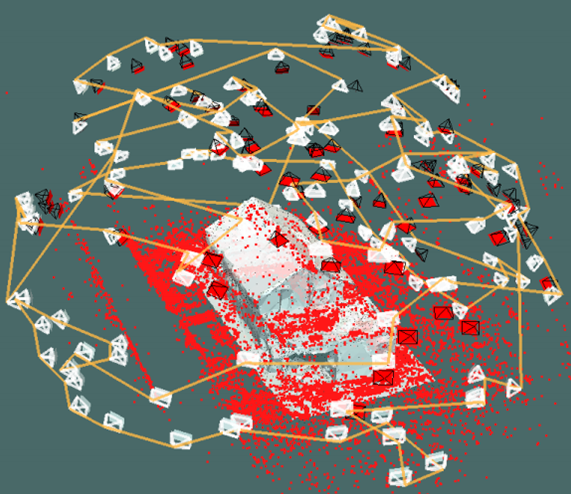
\includegraphics[width=\linewidth]{img/objectCoverFrom142.png}
  \caption{ Computed camera network pose estimation with the corresponding flight path (yellow) for an 3D object full coverage. This result is from Hoppe et al \cite{142*hoppe2012}. 
.}\label{fig:ObjectCover142}
  \endminipage\hfill
\end{figure}

\begin{itemize}
\item Object coverage: \\
   %The definition of a coverage can be varied this is a good example. 
   In Hoppe et al \cite{142*hoppe2012}  a good coverage is defined by  the ability to have full 3D reconstruction of an  object (in  their  3 dimension)  with no occlusion. This definition of the coverage is exploits the prior knowledge of the object to cover.  In this case the camera position will made a sphere around the object to cover as in the Figure \ref{fig:ObjectCover142}. 
   This definition of coverage  is not the more helpful due to this restricted application (focused only on 3D reconstruction). This formulation and solution applied is also not applicable for many object in the area. \\
   \item Path to cover: \\
   The coverage problem may be reduced as a series of path commonly borrowed by the users (car,  pedestrian, …). When the area to cover is a well-known place the path of the users can be deduced \cite{27*bodor2005} or if the area to cover is road the trajectory of the driver is knew \cite{14*lu2011}.  In this condition the aim is to cover the common path trajectory of the user as presented in  \cite{14*lu2011,27*bodor2005,30*bodor2005,81*nikolaidis2009}. The path coverage is interesting due to this numerous restriction of the area the coverage can became easier. Otherwise the path coverage introduce an important element is the zone with has a priority. This restricted zone in the area have to be cover in priority or only the path is taking in account in the area to cover.\\
   \item Coverage priority: \\
   A natural way of defining the coverage in a context of insufficient number of camera, is to define in priority some zone of interest to cover.
    In \cite{84*xu2011,165*jiang2010,171*horster2006} , their proposed to focus on priority on some predefined region, respectively called  region of interest, curial  sub-area (see Figure \ref{fig:MapRoI165}) and importance space weighting.  In the solutions proposed  by \cite{84*xu2011,165*jiang2010,171*horster2006}, the camera poses are in priority affected to this specific restricted region and neglected the other part of the area. \\
Logically if the environment is described with some region of interest some neutral zone must exist. The neutral zone (or normal sub-area) must be cover but their is not the priority. Furthermore some region can be describe as no interest region. In \cite{165*jiang2010,171*horster2006}  for example, the obstacle are designed as non-interested region and also this region have as consequences to occlude the vision of the camera. The main interest of this design is to keep a maximum of the  freedom in the cameras network positioning and see if the camera position can manage with the different local priority and constraints.\\
\item Inside or outside area:\\ 
Finally one of the most simplest  view of the coverage concern the outside and inside area coverage. The area to cover can be typically a room with walls. Each walls can be a considered as an obstacle and can occlude the camera field of view. In this case the main objective is to cover the surface in totality or at least maximize the coverage. This formulations is also workable for the vast outside area, but in addition it is necessary to take into account the size of the environment and the cameras limitation( as the depth of field), which can make the solution even longer and complex.
   
\end{itemize}
  


\begin{figure}[t!]
\minipage{0.85\textwidth}
   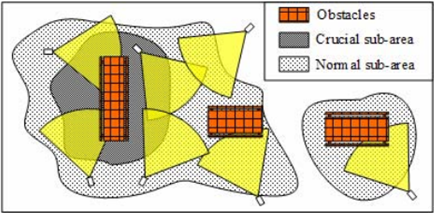
\includegraphics[width=\linewidth]{img/MapRoI165.png}
  \caption{ Map of an area to cover with  crucial sub area (region of interest) the normal sub-area  and obstacle. This map is an example of area coverage  introduce in  Jiang et al \cite{165*jiang2010}. 
.}\label{fig:MapRoI165}
  \endminipage\hfill
\end{figure}

The common point in all this coverage definition is the importance to maximize it, despite the other objectives. In the examples presented the coverage was always the first and for some of them the only objective. Despite the interest for maximize the coverage some other element have to be taken in account to have a useful cameras position depending on the finality. The secondary objective can have a not negligible impact on the camera pose. Depending on the camera pose will be greatly affected. The secondary objective are numerous and are closely related then the finality. The most interesting of them are listed:\\
\begin{itemize}
\item  The numbers of cameras: \\ In numerous situation the secondary objective is to limit the number of camera affected to the area as \cite{151*zhao2013,171*horster2006,22*zhao2008}. Limit the number of cameras is primordial to reduce the time computation for the final application and in some case the network traffic. Also reduce the number of camera to cover the full area mean reduce the cost of the video surveillance installation as \cite{82*chrysostomou2012}. In the case  minimizing the number of camera is a secondary objective not in contradiction with the camera pose optimization for coverage. The two objective can became complementary. But at some point a to strong trade-off in favour of the minimizing the numbers of cameras may reduce the area cover by accepting some small area  to be non covered (also called black hole). \\

\item Object tracking: \\ The secondary objective can be after the area coverage to detect and localize targets as for example in \cite{18*ding2012,12*soto2009,23*liu2009,39*wu2011,40*sohrabi2000,22*zhao2008}. In this case the secondary objective is to find a camera pose or dynamic adaptation of the pose for follow one or numerous targets. Keeping a full area covered and at same time the secondary objective is to track efficiently one or more target can became contradictory. The solution must be a trade-off between the coverage maximum coverage and the tracked following like in \cite{18*ding2012} and \cite{38*liu2010}. In Liu et al \cite{38*liu2010} the tracking of a target in a wide area is decomposed in phases, detection and location phase. For the detection phase, the area coverage is important but not any more for the location phase. These phases, although distinct for one target can intervene at the same time if there is more than one. Obviously when the secondary objective is to do tracking the cameras position will be less efficient for cover the area depending on the numbers of targets.  \\

\item  Luminosity and environmental setup:\\ Also  the  control of the image quality in terms of visibility can be an objective. Reddy et al \cite{33*reddy2012} are focus first on coverage of a complex area and in second time localize targets.  In order to manage what target must be follow the visibility is taking into account to avoid the too dark area, where the target is not enough visible at all. \\

\item  Energetic cost:
\\ To estimate the camera positioning another secondary element can be the energies cost in \cite{38*liu2010,42*bulusu2001}. Lui et al \cite{38*liu2010} is a good example, the first objective is to cover most of the area to be able to detect if a target is enter in the area. In second time the target is follow by the smart and autonomous cameras of the network. The set of cameras were randomly dispersed in the area and the coverage of the area will be to select the cameras useful for detect the targets intrusion in the area. The selection of the camera will be to manage between the maximum area overage and the minimum cost consumption.  Also the energy cost can be considered not in term of number of cameras turn on, but also in term of distance between each cameras. Notably in the case of each camera position will be a waypoint for doing a path planning \cite{191*di2016,218*meiting2007}.  
\\
\item Multi coverage:\\ Among the numerous secondary objectives possible the multi coverage is interesting (as for example in \cite{149*mavrinac2013,151*zhao2013,152*wang2009,174*zhang2016,175*medhi2013}). The multi coverage or also called K-coverage where $k$ represent the number of cameras useful to cover some region of the area. The multi coverage or $k$ coverage can be at some point confused with the region of interest and coverage priority. Mostly due to their importance given at some restricted part of area. The difference between them is the impact of the multi coverage on the finale coverage. The multi coverage involved one or few specific zone of the area to be covered by min $k$ cameras at same time in order to be considered as cover. This secondary objective in the case of limit will generate a conflict between the full coverage of the area and the k-coverage requirement even more with a restricted number of cameras. 
\\ 
\item  Resolution:\\ The objective of resolution is to keep the quality of the image acceptable \cite{27*bodor2005,33*reddy2012,171*horster2006,152*wang2009,43*erdem2006}. Most of his article are used the distance along the optical axis as a parameters in order to evaluate the resolution constraint. The lens, the sensor and the distance  between the camera  and a target (or surface) is used to estimate the resolution. In many application is essayer to adapt the distance between the camera and the target or the zoom (when the lens is not a fix focal ) then to modifies the other the sensor or the lens.\\
%The resolution is also model as the acceptable the depth of field.
  This secondary constraint affect mostly the system with positioning a set of cameras  comprising a zooming lens. If the constraint of resolution is not placed the interest to optimize the camera position for maximum coverage will be to zoom out (or place the camera highest) in order to cover  the wider region as possible. When the constraint of resolution is added a trade-off must be done between the zoom out or the camera distance to the target four maximize the coverage, and the zoom in to reduce the area cover for a better resolution.\\
   In \cite{33*reddy2012} the resolution is assimilated to be part of the image quality. In order to keep enough quality on the followed target,  the distance of the target is used to keep an acceptable resolution. The problem has been designed by using a Gaussian function in order to define the proper distance between the cameras and the target to keep an acceptable resolution for the application. \\
Also the depth of view have the same consequence on the camera positioning. Due to the focus point and the aperture of the camera (associate to the resolution), an object to close or to far became blurred. an ideal distance to the between the target and the camera is defined with some boundary  as in \cite{193*fu2014}. % (find ref 193)


\end{itemize}
The secondary objectives can be numerous and varied, where just few of them has been introduce (the more common and interesting). Among it, some of them are closely related and can be interconnected. The secondary objectives can be associate as in \cite{33*reddy2012} for example where the coverage target, luminosity, the resolution, and obstacle constraint are associate to find the best cameras position with maximize the coverage of the area and the target with good visibility condition. \\
The real interesting element about the secondary objectives is the impact in the cameras positioning for the global coverage of the area. Then the finality and the problem formulation will have a considerable impact of the obtained solution. Obviously the secondary objective have to be chosen carefully and there are related then the finality. To have an efficient cameras positioning system a trade-off between the different objective  and their importance have to be done in order to know what is the priority. In this case the problem became a multi objective problems. 


\section{Art gallery problem} \label{sec:AGP}
%Once the objectives defined the next step, is to know how to represent the problems. To do that manly 2 different class  of problems have to be studied. The first is from the geometrical problem called  the Art galery problms.


Until know the problem of coverage was studied to place cameras. The use of cameras (fix or mounted on mobile robot) are the limited field of view  and  depth field of the sensor. An interesting paradigm closely related is  to use human guards  instead  of the set of cameras.  This paradigm is called the Art Gallery Problem (called AGP). The AGP is an interesting  paradigm with propose some efficient solution. 

In the following section  a definition of the AGP is given with a brief historic. Next to this introduction on AGP some of the more interesting solution  are discussed before to see the limit of this paradigm.

%The problem of camera positioning is a tricky problem. The positioning of the set of cameras depend on many factor. To solve this problems is importatant to know more about the relat
% %finality of the camera networks and the formulation the camera pose will be affected.\\
%% Once the objectives defined ( see section \ref{sec:camerasPositioning}) the next step, is to know how to represent the problems. To do that manly 2 different paradigms have to be studied.
% The first is from the geometrical problem called the Art Gallery Problem (AGP) formulation is commonly and historically borrowed as is presents in the following section with a fast definition of the problems, the solution used and the limit of this paradigm.


	\subsection{Definition of the paradigm}
	The art gallery problem is a geometrical problem introduced by Victor Klee in 1973. The problem was to estimate the number (and the position) of useful guard to cover an art gallery. 
The particularity of a art gallery is the complexity of the room shape, with many wall to dispose the painting. The shape complexity of the room make the estimation  of guards number even more difficult.\\
In order to formulate properly the problem, the room is assimilate at a polygon $P$, composed by $n$ vertices ($v_1; v_2;…v_n$). The vertices are linked by  $n$ edges ($v_1 v_2;…; v_{n-1} v_n$) to make  the shape of the Polygon $P$ (or room).

A guard $x$ is inside the room $x \in P$. A guard $x$ can cover or see any point $y \in P$ if the segment $xy$ is not intersect by any boundary of the polygon $P$ (wall), in order to have $ xy \subseteq P$.
The polygon $P$ is considered as fully cover when for any position of the point $y$ in the polygon at least one guard can see him.\\
A guard $x$ can cover at $360^\circ$ all around him, with no depth of field limitation (except the wall obstacle). Clearly that mean the guard can see and monitor the entire length of the room one side to another side if no obstacle around to occlude. For example, if the shape of the room is a triangle, quadrilateral or another convex simple polygon, at any position taken by one guard, this guard can monitor all the area despite the size of the room. 

The minimum number of guards $X$ useful to fully cover the polygons $P$ is $G(P)$ with $k$ is the number of guard in order to have a set of points $X=\{x_1…x_i…. x_k\}$ so that every $y\in P$  are cover by at least on point of the subset of $X$. \\
The AGP  in addition  to estimating the numbers of guard also are interested on finding the optimal position of this  restricted number of guard. 
This 2 questions can be solve in the same time by using one of the solution proposed.


	\subsection{Solution }
	
	The main advances on the AGP since this formulation in 1973 are numerous. The following paragraphs present the major advance on it.\\
	 The first and one of the more important is the proof given by Chvàtal in 1975 \cite{44*chvatal1975}.  The polygon must have to be covered by a minimum of guard, the proof of Chvàtal propose to link the minimum number of guards to the number of vertices $n$. 
A polygon composed by $n$ vertices need in the worst case a minimum number of guard equal at $n/3$ The Chvàtal proof is based on the triangulation of the polygon. The Triangulation is made based on the vertices of the polygon.\\
	 % For a polygon composed by $n$ vertices in the worst case the minimum guard necessary to cover it, is $X=n/3$.
	     The proof given by Chvàtal is also confirmed by the work of Fisk  few years later (1978). The work of Fisk is also based on triangulation and colouring node. It is probably the easiest to understand and also give a solution to estimate the pose of each guard ( it is recommended to begin by the Fisk proof before the Chvàtal despite the chronologic order as it is preconized in \cite{219*orourke1987}). The book of O'ROURKE et al \cite{219*orourke1987} is an early work about the AGP with the formulation, proof and advancement of the field clearly explained. \\
Once the proof of the minimum number in the worst case found the objective became to find an optimal solution in reasonable time. \\
For that the work of Toussaint and Avis (in 1981) is the reference and propose a solution working in $O(n log n)$. This work has been follow and upgrade until the solution of Couto, Resend and Souza  2011 \cite{224*couto2011} a solution is finally proposed in $O(n^3)$  in the worst case. 

%It is a short overview of the AGP solution but also the solution proposed are very specific to the AGP and cannot be re-use for problem little different.

	
	\subsection{limit of AGP and camera coverage relation}


The problem of positioning camera for coverage estimation is quite close then the AGP. In many ways, the AGP is a reduction of the camera positioning for a total coverage of a complex areas. The camera positioning is the logical continuation of AGP and once some AGP is knew, the problem can be extended as is for  example show in \cite{221*fleishman2000,33*reddy2012,43*erdem2006}.

The algorithm developed for AGP cannot be applied directly on the problem of cameras positioning for maximum coverage. The main reason is the cameras limitation field and depth of view (\cite{82*chrysostomou2012,170*yabuta2008} which makes is unreadable the solution proposed of solve AGP, where AGP considering the guard with no limitation for the depth of field and field of view. \\
Also another reason make the AGP solution not applicable for the camera positioning is the diversity of cameras. In the same system the AGP may have many guard, they are all interchangeable because it has all the same ability (or skill) to monitor the area. This weakness in the AGP formulation associate to the limited field of view  make the solution form AGP note adapted as  is showed in \cite{81*nikolaidis2009,171*horster2006}.\\
Due to this limitation, the solution developed for AGP are not applicable. However the formulation and some proof has their importance. 
Despite that, numerous article are based on the AGP to formulate the problem as in \cite{43*erdem2006,53*packer2008}. For example in \cite{43*erdem2006} the similar approaches then the AGP is used  in order to estimate the occluded   region. Also in \cite{53*packer2008} (page 105)to estimate the area covered a grid of $y= (y_1 ...y_i)$ is used in order to discretise the area. this method is directly based on the AGP formulation.\\
Also one important impact of AGP is the shape of the room. In \cite{170*yabuta2008,171*horster2006,33*reddy2012,43*erdem2006} the shape of the room are close then the definition of an art gallery. This phenomena can be imputed to the link did between the number of vertices and the useful number of guards (or cameras) to cover it. \\
The room composed with numerous wall inside create few occlusion. The occlusion mean the segment $xy \not\subset P$   where $x \in P$ is the camera position $y \in P$ is a points in the room $P$. The occlusion is one of the element make the camera positioning really complex. The use of room inspired by  AGP is therefore a good choice in order to verify the effectiveness of the system in a complex environment.\\
The complexity of this problem is also an important factor which makes the relation of camera positioning and AGP. \\
The AGP is NP-hard problems \cite{219*orourke1987}). The NP-hard proof is available on the book of O’Rourke section 9.2 of the book \cite{219*orourke1987}). \\
To proof the AGP is  NP-hard, the first part is to reduce the  problem to an other problem welle known for this complexity. The relation is made by reducing the AGP with a polygon composed by  holes to another standard problem ( in the demonstration the is used 3SAT). \\
Once the AGP is reduced to 3SAT and because 3SAT is an NP-complete problem the AGP is  also considered as NP-complete or  NP-hard but only  when the room is composed with holes. Also another work of Lee and Lin 1986 proof the complexity of AGP without hole also by reducing the AGP ton an other well known problem (for more explication see the book of O’Rourke  section 9.3 \cite{219*orourke1987})).

As we explained earlier the camera positioning can be reduced as an AGP \cite{53*packer2008} notably by removing most of the constraint due to the camera properties. \\
In the literature numerous article us the AGP reference to explain the complexity of the problem as for example \cite{26*moeini,44*chvatal1975,149*mavrinac2013,151*zhao2013}  assumed the problem is at least NP-complete or NP-hard. 
The complexity of the problem will have an impact on the solution used  to try to solve it and optimize it.

The AGP can be at same time  for part the  historical source of the cameras positioning and give some answer about the problem this formulation and this complexity. Despite that, the AGP is not the only source to refer about the cameras positioning for maximize the coverage. Some clue and solution can be find in other related field. 




\section{Wireless sensor network   }

The wireless sensor network (WSN) can be as AGP considered as inspiration for the cameras positioning problem. The WSN is an active field of research and in many aspect related to the cameras positioning. This parties is focused on the WSN and this relation with the camera positioning.  But first allow  :

What is the Wireless Sensor Network? 

 The WSN is a distributed network of sensor or in some case actuator, in this case is also called WSAN. Each sensor of the network is a relay for the information and commend, to the rest of the network.  
The sensor are at same time the node for the network. The node have to objective to transmit by relaying the information to the other node or to a centralized agent.  Furthermore the node have to be the sensor for collect information and decided to communique with the other node. 
The information collected by the sensor are vast (extensive) depending on the final application and the capacities of the sensors ability. 
The WSN is used in different field for various application as for telecom and antenna positioning \cite{59*wang2008} military surveillance field \cite{38*liu2010,101*topcuoglu2009}, airport surveillance \cite{37*ma2012}, video surveillance and tracking \cite{38*liu2010}, environmental monitoring \cite{42*bulusu2001}... Logically numerous sensor and information can be collected  as temperature, movements, images, song and also some  actuator can be used as radio frequency for example.\\
 The application of WSN are wide, especially since the WSN has more than one discipline. The WSN try to optimize a network of sensor in different aspect as for example \cite{39*wu2011} focus on an architecture adapted and efficient enough for data transfer (image) or like in \cite{40*sohrabi2000} the WSN are dedicate to adapt the network around static node and energetic resources in order to keep the network connected.  \\
For our case the discipline the more interesting is the coverage of an area with his specific constraint of the WSN for maximum coverage.\\
 The other discipline of the WSN as the network optimisation will not be addressed in the following section. Only the problem of coverage is studied  the other discipline are not considered as the first or main objective but can be some secondary objectives after the problem of coverage.

	\subsection{Sensor at 360}
	\begin{figure}[t!]
\minipage{0.55\textwidth}
   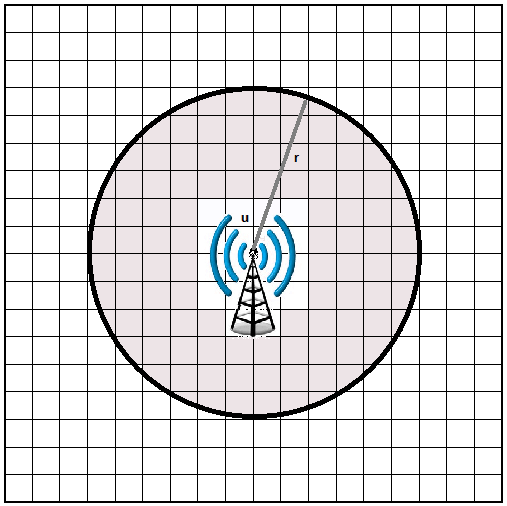
\includegraphics[width=\linewidth]{img/WsnSensor1.png}
  \caption{ one omnidirectional sensor centred on $u$, with a radius $r$ for the range.}\label{fig:WsnSensor1}
  \endminipage\hfill
\end{figure}

The wireless sensor network (WSN) refer commonly to sensor or actuator  with no restriction in the view angle, it is considering to have a $360^\circ$ of field of view  as in \cite{200*kulkarni2011, 174*zhang2016,150*chakrabarty2002} (see Figure \ref{fig:WsnSensor1}) and in some case a spherical as example in \cite{175*medhi2013,59*wang2008}.  \\

Each sensors have a position $u$ in the area and a power. From the sensor power the radius $r$ of the circle is deduced from $u$ as center (show \ref{fig:WsnSensor1}). This circle give the area cover by a sensor in the simplest case. 
The simplest case correspond to a flat area without any obstacle, or it is negligible and do not impact the covered area as in \cite{200*kulkarni2011,174*zhang2016}.  
Others more complex solutions can be used. Its are more complex but also more realistic as in \cite{59*wang2008} where are taking in account the relief and obstacle. 
In \cite{174*zhang2016} more complex model have been developed, where despite of a flat ground without obstacle each sensor is composed by a perception radius and a communication. The communication radius a bit bigger then the perception radius. This 2 radius correspond to area covered for one antenna (sensor) and the distance of emission/reception of the data.  In order to have an efficient coverage of the area, the antenna must be place in order to have connection with other antenna but without too much overlap of the perception sensor.\\

The solution proposed in order to optimize the positioning of the WSN for a circular sensor can be varied. Mostly 2 different ways are applied for the sensor with have circular angle of view or spherical.\\

\begin{itemize}



\item	The first solution use an heuristic based on geometry construction as in \cite{175*medhi2013}. This approaches give a good coverage solution but is usually greedy and can be quickly limited in term of number of sensors, moreover if some external constraint are added.  For example in \cite{174*zhang2016} the greedy solution was tested and optimized by using a "partition and shifting" strategy in order to upgrade the result.
The limit of this solution despite the greedy consumption resources is also not applicable to the problem of camera positioning due to the reduced field of views of a cameras.  \\
\item	The second solution try to find an efficient and quick solution to optimize  random position for each sensor of the network.  
This solution include many different family of algorithms focused on optimization.
Among the family of algorithms,  the evolutionary algorithms (disused in detailed in section  \ref{chap:EA}) is commonly used as in \cite{200*kulkarni2011,59*wang2008}, and \cite{150*chakrabarty2002}. \\
These solutions  propose to optimize the position in order to maximize the coverage depending on different constraint or the secondary objectives. The method of optimization have to be adapted to the problem. 
In  \cite{150*chakrabarty2002} the integer linear programming with an "LPsovlver" are chosen in order to maximize the coverage with 2 type of sensors. One standard with a smaller area coverage but with a smaller cost (can have a $100m$ radius for 150\$) and the other sensor can cover a wider region (can have a $200m$  radius for 200\$) and the objective is to cover the region but also to reduce the cost. The solution proposed is to use the integer linear programming adapted to the problem of coverage optimization with the economic cost in constraint. \\
In \cite{59*wang2008} and \cite{200*kulkarni2011} the solution proposed is based on 2 different evolutionary algorithm in order to optimize the sensor positioning. In \cite{200*kulkarni2011} the camera positing with a multi coverage is solved with using an evolutionary algorithm called particle swarm optimization (PSO). The objective is to optimize the position of the sensor in order to have an efficient coverage of the area and also enough redundancy to keep the network workable if one or few sensor fail. In \cite{59*wang2008} one evolutionary algorithms is also used to optimize the potion of antenna. The objective in this paper is to give the best coverage of an area with taking in count the relief of the area. The relief make the coverage estimation of each sensor even more complex and costly in terms of time computation. The Genetic algorithm are used in order to find quickly a position for each antenna of the network. 
\\
\end{itemize}

Among the examples seen the second solution based on optimization is the more interesting and also the more flexible to new constraints and secondary objective. The aim is to see up to what point and if it is applicable to the problem of cameras network positioning.  

	\subsection{Visual sensor network}
	
Logically, the result obtained with the Omni-directional sensor are interesting and  must be applied to the problem with even more constraint and objective as can be the  positioning of visual sensor network (VSN).  In fact the visual sensor or camera have a limited depth of field but also a limited field of view. This new constraint make the sensor positioning more complex as that was for AGP (see section \ref{sec:AGP}) to passes from guard to camera. The advantage in this case,  are first the sensor have been designed with a limited depth of field. Also the solution applied previously for circular sensor was not only geometric or based on heuristic but also the problem is formalized as optimization problems with some solution based on optimization and meta-heuristic. This way to present the problem is appear as the more suitable to add constraint and secondary objectives. Also the solution and the formulation for the problem of VSN are mostly the same then the problems of cameras positioning and is  discussed in the following parts  \\
  

	\section{Solution not based on evolutionary method}
	
The solution used to pose a set of cameras to maximize the coverage are various but  among the possible solution manly two way can be describe. The solution proposed they come from numerous sources and paradigm  which AGP and WSN.\\
 The first is to construct a solution as an heuristic to have an appropriated cameras position. The second way is to formalize the problem as optimization problem and applied meta-heuristic. 

\subsection{The constructive solution}

The cameras pose can be done by construction. By construction that mean a deterministic method is applied to pose one camera after the other or to adjust their position.\\
In \cite{38*liu2010} a constructive solution is applied in order to select the smart cameras of the network. Each smart camera area a node of the network and transmit information, image and are fully autonomous. 
They work in 3 different modes:\\
\begin{itemize}
\item[-] The first is the sleepy mode. The sleepy mode is used in order to economize a maximum of the energy. To do that the camera is turn off. That mean no computation and just the network is listen at regular intervals to wait the wakeup call.   \\

\item[-] The Second is the detection mode the camera is turn on, but with a low frame rate. Just a few computation is done to detect if a target is enter in the field of views. Some information may be transmit by network. This mode consume more energy of the previews but the smart cameras can stay in this mode during a long time.\\

\item[-] The last mode is a tracking mode. This mode is the more energy consumer. The camera is turn on, with a high frame rate and numerous computation have been done to track and localize the target. Also more information have to be transmit by the network. The information are useful to localize the target by communicate with  the potential other smart cameras with a view on the target. \\
\end{itemize}
The objective in \cite{38*liu2010} are multiples depending on the state of the cameras. the one the more interesting for us is to keep under control the longest time as possible the area for target detection. Numerous smart camera are randomly dispersed in the area (as an air-drop in a battlefield) and the aim is to select the camera in order to maximize the coverage of the camera in detection mode. The solution proposed by LIU  et al in \cite{38*liu2010}.
To do that the solution used is by construction with using a talk between each smart cameras of the network. Also each sensor is capable to estimate precisely this localization, it is an important element to select the cameras. The solution proposed is inspired of the network distributed talk. \\
To begin all sensor are in sleepy mode.  The camera wake up regularly and send a call at the neighbour, if they receive no answer that mean no other camera is awake around and the camera stay in detection mode. If no enough answer have been received, that mean the required density of the camera around are not enough the camera stay turn on detection mode. Otherwise the camera return on sleepy mode until another wake-up later. This procedure is applied in each smart camera with all have their own pace. After a certain time the network is well organize to cover the area in detection mode.
 The method introduce by LIU et al in \cite{38*liu2010} work well. the solution proposed have the advantage to can  work in wide area and to be dynamic (if one cameras do not have any-more power the network ll re-adapts).  \\
The solution are efficient  with a high density of sensor to have a relatively low coverage (just enough to detect target in the sparse sensor placement). Also the method presented is really dependent then the network communication and the capability to localize precisely each sensor. Finally the solution proposed to select a set of sensor among a randomly posed sensor is not enough optimized.\\

Another cameras pose estimation by construction is proposed by HÖRSTER et al \cite{171*horster2006}.
The solutions proposed is based on a greedy search heuristic.  The objective is to find a position and orientation of a set of cameras with a fixe pan, in the environment inspired by the AGP. \\
In \cite{171*horster2006} a first greedy search solution have been presented then finally a solution called Dual Sampling has been presented based on it.
The dual sampling is an incremental method. \\
First step is to initialize the position of all the cameras. A random initialization for the position and the orientation must be appropriate.  \\
Second step is to select one point of the area. The area is discretized by numerous points, with each point must be covered by at least one camera. Around the selected point several position and orientation are tested for the cameras at proximity. The possible position are obtained by sampling the area around the point to cover. Finally the best cameras position and orientation is kept.
The second step is repeated and the set of uncovered control point is reduced an each iteration.  This procedure is applied until the stop criterion is reach that mean enough points of the area are covered. \\
This constructive solution have some inconvenient notably in terms of efficiency. Indeed this solution is limited by the number of camera and size of the area due to the exponential complexity.\\

In \cite{81*nikolaidis2009} the camera placement to cover a basic mobile robot trajectory is studied.
The trajectory is modelled as the region of interest, with a gradually decreasing interested from the trajectory center.\\
  The solution applied in  \cite{81*nikolaidis2009} is to do a local optimization one camera after the other with the “steepest decent method (decent de gradient)”. If this local optimization give a better solution the network of camera is modified otherwise the camera stay at the same place. This operation is repeated until the convergent arrangement is obtained or no more upgrade can be found. This result presented in the experiment done by Nikolaidis in  \cite{81*nikolaidis2009} are interesting despite the simplicity of the area and the very small amount of camera used.  The principal limitation is due to the number of step required for optimize independently each camera of the network. Also a multitude of local optimisation is not obviously the same then the global optimization.\\

Ma et al \cite{37*ma2012} propose a solution for the problem of finding the minimum camera barrier coverage. The objective is to cover only the boundary of an area, to be able to detect target intrusion in the perimeters. The perimeter is relatively wide and can be considering at some point as an area to cover composed by big hole in this center.\\
 The region to cover is cut in numerous sub-region. The region are inter connected, each sub-region have to be “full-view covered”. The full view covered is define if for any target direction there always exist a sensor cover to the face of it.\\
The solution purposed is based on constructive solution with adapted heuristic (the heuristic used is presented on \cite{37*ma2012}). The global idea is to cut the perimeter in different sub-region and applies the method presented to full view cover  each sub region. 
The cutting on sub-region offer at the heuristic to work in reasonable time due to this restricted area.\\
The solution proposed though this efficiency in the case of barrier coverage is not rely appropriate to vast coverage area. The first limitation is the number of cameras use to fully cover the area. The number of cameras is mainly due to this definition of “full view covered” . That definition  imply many overlap to have the multi direction coverage.\\


As show, the previous solution are based on constructive method for the camera placement and their local optimization. Each camera is placed dependently then the network with an iterative process in order to have a position for each camera of the set. This methods have some consequence, nobly the fast increasing number of iteration useful to have a solution good enough. The time complexity is event more problematic with  increasing the size of the area. Also these solution are extremely dependent then the formulation and the constraints and cannot be easily adapted to other problems. 

\subsection{ !!! Linear programming optimisation !!! (to verify)}
	Different method of linear optimization was applied and test. In some case due to a well-adapted formulation; a specific shape of the area or cameras number The linear optimisation is efficient. 
	The linear optimisation has been commonly used to have initial result in order to have a reference point before to develop other solution more appropriate(as example \cite{141*akbarzadeh2013,151*zhao2013,82*chrysostomou2012,33*reddy2012}…).  \\
%	The reason ofIn some other case the method was studied but finally rejected du to this fast limitation 
	 The linear optimisation  is finally rejected due to this fast limitation.  Indeed the linear optimization can be quickly in difficulty due to the fast increasing complexity of the problem and in many case be lock in local minima. as presented in the flowing example.\\

%%\textbf{!!!!!! partie manguante sur l'utilation des methode linear  !!!!!(voir path planning)}
	 
	 
The \cite{43*erdem2006} is based on AGP and the WSN and propose a fusion off their 2 paradigms in order to use there assumptions. Some modification have been done as example to taking in account the field of view limitation. The interesting aspect is how some camera properties have been modeled to fit to the problem of AGP.  \\
The solution proposed is workable with using an omnidirectional or considering a PTZ as omnidirectional cameras by using an efficient angular sweep. The simulated omnidirectional cameras is simulate by PTZ camera with a non-continue zoom or fix focal length as in the  experimentation (see fig 7) where  the PTZ can have a focal two focal length  at 50mm and  35mm. 	 \\
	 

Finally the solution proposed is to discretize the area to cover (fig 7 left) and also the different possible parameter for the camera (as: localization, orientation, focal...). Thanks to this discretization and a formulation close then the binary integer programming (BIP) and apply a well-known method “Branch and Bound” in order to optimize the camera placement.  \\
This solution  propose a  good  coverage with the minimum of cameras  in reasonable time until, the  number of location sample ( point in the grid on the floor) , the numbers of camera, and the number of parameter possible for the camera stay relatively  reduced.  \\
 
Zhao  et al \cite{22*zhao2008} are trying to find the optimal position for a set of camera in order to maximize the  Indore coverage (like an AGP room) and also to  do tag detection.
The solution proposed for the coverage is to adapt the number of point of interest wish must be covered by the camera. \\
The area is discretize in grid.  The grid is composed by point selected smartly depending on the coverage rate. Each point of the grid simulate a potential location of the target.\\
Also a limited number of possible position for the camera (the boundary of the room) are defined.
The adapted grid and the limited camera positioning is used to limit the complexity ( as number of possible solution).  linear optimization to the Binary integer problem formulation. \\
Use a Binary integer problem formulation (BIP) in order to apply a linear optimization is popular and other use it as in \cite{22*zhao2008,27*bodor2005,43*erdem2006}. In \cite{22*zhao2008} the solution proposed is to use BIP formulation the grid smart sampling and LP\_solve to optimize the camera position and orientation.\\

 A Similar method is used in \cite{27*bodor2005} to find the position and orientation of a set of cameras. The goal of this paper is to find the appropriate position with maximize the resolution for a set of cameras dedicate to do tracking. The position is determined depending on a set of standard pedestrian trajectories. The camera pose try to maximize the given trajectory to have the best resolution and the entire coverage. \\
The problem is also formulate in order to apply a linear well-known algorithm. In this case the branch and bound is applied.  

\subsubsection{	Limitation of linear method}
Different method of linear optimization was applied and test to answer, the problem of camera position for maximum coverage. In some case due to a well-adapted formulation or a restricted area and cameras number this solution is efficient enough. In some other case the method was studied but finally rejected due to this fast limitation (as example \cite{141*akbarzadeh2013,151*zhao2013,82*chrysostomou2012} …). Indeed the linear optimization can be quickly in difficulty due to the fast increasing complexity of the problem and in many case be lock in local minima.

	
In WANG et al \cite{181*wang2017} propose a solution with an atypical problem formulation. The solution proposed in \cite{181*wang2017} is mainly based on the method of discretize the area. The idea is to have an area discretized with precision with use the minimum of point. To do that the solution proposed is to decompose the area in order to give more point in the grid were the shape of the room need it to be correctly described. \\
The principal advantage of this solution is to propose an area representation with enough precision and a minimum of point to describe it. Less point to describe the area to cover mean also a winning time efficiency in computation during the camera pose estimation (cost function is faster).
Despite this interesting solution the result presented in the experiment does not appear to be conclusive. \\
	
\subsection{Game theory} 
	 
Among possible solution an atypical method is to use the game theory \cite{19*li2013}. The game theory is use to optimize the looking direction of the cameras as in \cite{12*soto2009,18*ding2012,19*li2013,25*song2008}. These articles are based on game theory to find an equilibrium (also named Nash equilibrium) between two contradictory objectives, the maximize the resolution and the multi target tracking.\\

Soto et al \cite{12*soto2009} propose a network of a dozen of PTZ cameras. The PTZ is for pan tilt zoom, that mean the position of the cameras are fix and the solution proposed is to find the best orientation with the appropriate focal lens to track most of the targets.  \\
 To do that the camera are smart enough to communicate with the close neighbours and adapt the pan, tilt, zoom depending on the needs.\\
The need has been defined by an utility function (or local cost function). The goal is to track most of the target as possible with the better resolution. The cameras scores when it obtained a desired resolution image for all the targets visible by the networks.\\
The trade-off proposed is between the multi tracking and the best coverage resolution for each target. The multi-target problematic can appear far from maximization of the coverage. But the number of targets  which may be higher than the number of cameras, push the camera tracking to be an interesting solution to maximize the coverage of an area. In this case the quality of the coverage will also dependent then the number of targets and the importance of the resolution constraint.  \\
	 In \cite{18*ding2012} and \cite{25*song2008} different experiment have been proposed with a number of target is lightly increased.  In this articles the game theory is applied to trade-off between the tracking and the resolutions. The proposed experiment is based on the decentralized method. It is justified by the complexity to dynamically adapt all the camera of the network at same time depending on each targets trajectories.\\
	  Furthermore, the decentralized solution is more adapted for the security of the transmission and the risk of interception by a hostile opponent. The security may be an important factor in some applications. \\
To have the decentralized system the camera must have some autonomy. \\
In the experiment proposed in \cite{12*soto2009} and \cite{18*ding2012,25*song2008}  each camera are smart enough to have their own tracking  and control module. Also the camera are able to communicate with each other to come to a consensus. The consensus is when a Nash equilibrium is found between the 2 contradictory objectives. In this case it is a win win situation for both objectives.\\
So the objectives are not independently optimize, moreover  the  solution proposed is to optimize its  simultaneously in order to have a consensus. The consensus is reach when it became impossible to upgrade one of them without downgrade the other one.\\
  In the experiment of \cite{18*ding2012,25*song2008} the consensus is found by the camera communication in order to have a maximum of the target cover with the higher resolution.
 The experiment is based on numerous target moving freely in the area. Also in \cite{18*ding2012} one of the target must be cover in priority with a high resolution. That will have an impact on the other camera position.
 The result of the experiment as in figure \ref{fig:CoverageFrom18} form \cite{18*ding2012} show a really efficient global coverage with almost all the target cover at every time despite the movements of the targets. \\
 The advantage of these solutions is the acceptable result and dynamic reconfiguration of the system for the reasonable size of the area and the decentralized computation.\\
Otherwise this method have some limit, as show in the experiment the area is relatively restricted and numerous cameras with a fixed position are useful. The consequences is the quantity of overlap relatively important. In this case the number of sensor is not well optimize to cover the area. Also to use properly this method for maximum coverage it requires a large number of simulated target in the region to observe. 

\begin{figure}[t!]
\minipage{0.55\textwidth}
   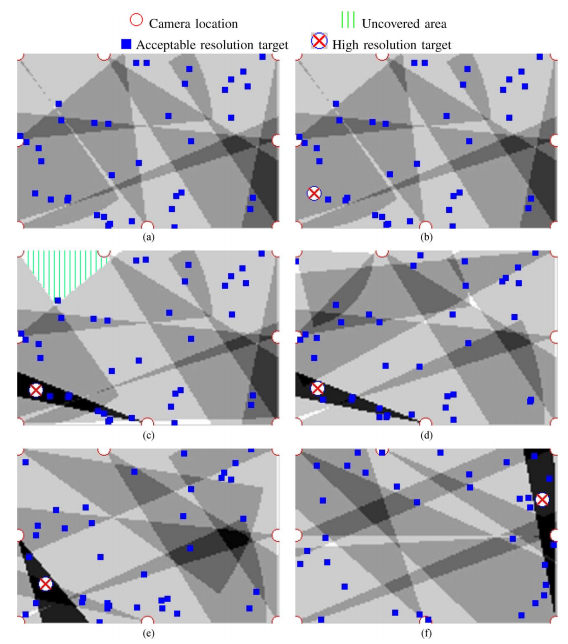
\includegraphics[width=\linewidth]{img/CoverageFrom18.png}
  \caption{ result of coverage after have used the game theory with objective to maximize the tracking and the resolution. result obtained in the experiment presented in \cite{18*ding2012}}\label{fig:CoverageFrom18}
  \endminipage\hfill
\end{figure}
	
	%%%%%%%%%%%table sum up%%%%%%%%%%%%%%%%%%%%%%%%%%
	% Please add the following required packages to your document preamble:
% \usepackage{booktabs}
% \usepackage[table,xcdraw]{xcolor}
% If you use beamer only pass "xcolor=table" option, i.e. \documentclass[xcolor=table]{beamer}
%\begin{landscape}
%
%	\begin{table}[]
%\centering
%\caption{Sum up articles.}
%\label{my-label}
%\begin{tabular}{@{}lp{2.6cm}lllp{1.6cm}p{1.6cm}llp{1.3cm}p{1.3cm}p{1.65cm}p{1.6cm}p{1.3cm}p{1.3cm}p{1.4cm}@{}}
%\toprule
%\multicolumn{1}{|l|}{\textbf{ref}}               & \multicolumn{1}{l|}{\textbf{\begin{tabular}[c]{@{}l@{}}Best \\ solution\end{tabular}}} & \multicolumn{1}{l|}{X} & \multicolumn{1}{l|}{Y} & \multicolumn{1}{l|}{Z} & \multicolumn{1}{l|}{\begin{tabular}[c]{@{}l@{}}Point\\  selection\end{tabular}} & \multicolumn{1}{l|}{Pan} & \multicolumn{1}{l|}{Tilt} & \multicolumn{1}{l|}{Roll} & \multicolumn{1}{l|}{focal lenght} & \multicolumn{1}{l|}{\begin{tabular}[c]{@{}l@{}}Coverage\\  representation\end{tabular}} & \multicolumn{1}{l|}{\begin{tabular}[c]{@{}l@{}}number of \\ cameras\end{tabular}} & \multicolumn{1}{l|}{\begin{tabular}[c]{@{}p{1.65cm}@{}}Secondary objectives \\ and contraints\end{tabular}} & \multicolumn{1}{l|}{} & \multicolumn{1}{l|}{} & \multicolumn{1}{l|}{} \\ \midrule
%\rowcolor[HTML]{FFFFFF} 
%\multicolumn{1}{l|}{\cellcolor[HTML]{FFFFFF}37*} & heurisitic                                                                             & x                      & x                      & 0                      & 0                                                                               & x                        & 0                         & 0                         & fix                               & 2D                                                                                      & around 10 (per section)                                                           & barrier coverage                                                                                    & conection dependance  &                       &                       \\
%\multicolumn{1}{l|}{\cellcolor[HTML]{F2F2F2}38*} & \cellcolor[HTML]{F2F2F2}heuristic                                                      & \cellcolor[HTML]{F2F2F2}0                      &\cellcolor[HTML]{F2F2F2} 0                      &\cellcolor[HTML]{F2F2F2} 0                      & \cellcolor[HTML]{F2F2F2}\begin{tabular}[c]{@{}l@{}}random \\ dispersion (x;y)\end{tabular}              &\cellcolor[HTML]{F2F2F2} 0                        &\cellcolor[HTML]{F2F2F2} 0                         &\cellcolor[HTML]{F2F2F2} 0                         &\cellcolor[HTML]{F2F2F2} fix                               &\cellcolor[HTML]{F2F2F2} 2D                                                                                      &\cellcolor[HTML]{F2F2F2} around 600                                                                        & \cellcolor[HTML]{F2F2F2}resolution                                                                                          & \cellcolor[HTML]{F2F2F2}tracking              &  \cellcolor[HTML]{F2F2F2}                     &                      \cellcolor[HTML]{F2F2F2} \\
%\rowcolor[HTML]{FFFFFF} 
%\multicolumn{1}{l|}{\cellcolor[HTML]{FFFFFF}27*} & non-linear                                                                             & x                      & x                      & 0                      & 0                                                                               & x                        & 0                         & 0                         & fix                               & 2D                                                                                      &                                                                                   & tracking                                                                                            & resolution            &                       &                       \\ \rowcolor[HTML]{F2F2F2}
%\multicolumn{1}{l|}{ \cellcolor[HTML]{F2F2F2}43*} & \cellcolor[HTML]{F2F2F2}game                                                           & x                      & x                      & 0                      & 0                                                                               & x                        & 0                         & 0                         & x (discret)                       & omni directional (mobil pan)                                                             & around 10                                                                         & cost reduction                                                                                      & resolution            & DoF                   &                       \\
%12*                                              & game theori                                                                            & 0                      & 0                      & 0                      & 0                                                                               & x                        & x                         & 0                         & x                                 & 2D                                                                                      & around 10                                                                         & resolution                                                                                          & tracking              & multi target          &                       \\
%\rowcolor[HTML]{F2F2F2} 
% 18*                                              & game theori                                                                            & 0                      & 0                      & 0                      & 0                                                                               & x                        & x                         & 0                         & x                                 & 2D                                                                                      & around 10                                                                         & resolution                                                                                          & tracking              & multi target          &                       \\
%25*                                              & game theori                                                                            & 0                      & 0                      & 0                      & 0                                                                               & x                        & 0                         & 0                         & x                                 & 2D                                                                                      & around 14                                                                         & resolution                                                                                          & tracking              & multi target          &                       \\
%\rowcolor[HTML]{F2F2F2} 
%81*                                              & heurisitic                                                                             & x                      & x                      & 0                      & 0                                                                               & x                        & 0                         & 0                         & fix                               & 2D                                                                                      & 2 to 4                                                                            & Region of interst                                                                                   & trajectory coverage   &                       &                       \\
%22*                                              & LP-solve                                                                               & x                      & x                      & 0                      & 0                                                                               & x (16 orientation)       & 0                         & 0                         & fix                               & 2D                                                                                      & around 10 (8-11)                                                                  & tag detection                                                                                       & tag visbility         &                       &                       \\
%\rowcolor[HTML]{F2F2F2} 
%170*                                             & linear programming relaxation                                                          & x                      & x                      & 0                      & 0                                                                               & x                        & 0                         & 0                         & fix                               & 2D discret square                                                                       & around 20                                                                         & Region of interst                                                                                   &                       &                       &                       \\
%171*                                             & LP-solve                                                                               & x                      & x                      & 0                      & 0                                                                               & x                        & 0                         & 0                         & x (discret 3)                     & 2D                                                                                      & around 10                                                                         & cost reduction                                                                                      &                       &                       &                       \\
%\rowcolor[HTML]{F2F2F2} 
%181*                                             & Multistage Grid Subdivision                                                            & x                      & x                      & 0                      & 0                                                                               & x                        & x                         & 0                         & x                                 & 2D                                                                                      & 9 to 15                                                                           & Region of interst                                                                                   & big area              &                       &                       \\ \cmidrule(r){1-13} \cmidrule(l){16-16} 
%\end{tabular}
%\end{table}
%	
%\end{landscape}	
	
	
	%%%%%%%%%tab v2 %%%%%%%%%%%%%%%%%%%%%%%%%%%%%%
\begin{landscape}	
	\begin{table}[]
\centering
\caption{Sum-up ref}
\label{tab:sum-up1}
 %              ref           |x|y |z| pan|      tilt| |focal  coverage     nmb   
\begin{tabular}{@{}l|p{2.4cm}  l  l l p{0.659cm}p{0.62cm}lp{1.3cm}p{1.57cm}p{1.5cm}p{1.6cm}p{1.3cm}p{1.2cm}@{}}
\toprule
\multicolumn{1}{|l|}{\textbf{ref}} & \multicolumn{1}{l|}{\textbf{\begin{tabular}[c]{@{}l@{}}Best \\ solution\end{tabular}}} & \multicolumn{1}{l|}{X}              & \multicolumn{1}{l|}{Y}              & \multicolumn{1}{l|}{Z}             & \multicolumn{1}{l|}{Pan} & \multicolumn{1}{l|}{Tilt} & \multicolumn{1}{l|}{Roll} & \multicolumn{1}{p{1.29cm}|}{focal lenght} & \multicolumn{1}{l|}{\begin{tabular}[c]{@{}p{1.55cm}@{}}Coverage\\  room\end{tabular}} & \multicolumn{1}{l|}{\begin{tabular}[c]{@{}l@{}}number\\ of \\ cameras\end{tabular}} & \begin{tabular}[c]{@{}l@{}}Secondary objectives \\ and constraints\end{tabular} &                      &               \multicolumn{1}{l|}{} \\ \midrule
\rowcolor[HTML]{FFFFFF} 
\cite{37*ma2012}                        & heuristic                                                                             &  \ding{52}                                   & \ding{52}                                   & 0                                  &  \ding{52}                        & 0                         & 0                         & fix                               & 2D                                                                                      & $\approx 10                                                                        $                                                           & barrier coverage                                                               & conection dependance &                                     \\
\rowcolor[HTML]{EFEFEF} 
\cite{38*liu2010}                                & heuristic                                                                              & \multicolumn{3}{l}{\cellcolor[HTML]{EFEFEF}\begin{tabular}[c]{@{}l@{}}random \\ dispersion (x;y)\end{tabular}} & 0                        & 0                         & 0                         & fix                               & 2D                                                                                      & $\approx 600                                                                        $ & resolution                                                                     & tracking             &                                     \\
\rowcolor[HTML]{FFFFFF} 
\cite{27*bodor2005}                                & non-linear                                                                             &  \ding{52}                   &  \ding{52}                                   & 0                                  &  \ding{52}                        & 0                         & 0                         & fix                               & 2D                                                                                      &                                                                                   & tracking                                                                       & resolution           &                                     \\
\rowcolor[HTML]{EFEFEF} 
\cite{43*erdem2006}                               & game                                                                                   &  \ding{52}                                   &  \ding{52}                                   & 0                                  &  \ding{52}                        & 0                         & 0                         &  \ding{52} \newline(discret)                       & omni directional (by pan)                                                             & $\approx 10                                                                        $ & cost reduction                                                                 & resolution           & DoF                                 \\
\rowcolor[HTML]{FFFFFF} 
\cite{12*soto2009}                              & game theory                                                                            & 0                                   & 0                                   & 0                                  &  \ding{52}                        &  \ding{52}                         & 0                         &  \ding{52} & 2D                                                                                      & $\approx 10                                                                        $ & resolution                                                                     & tracking             & multi target                        \\
\rowcolor[HTML]{EFEFEF} 
\cite{18*ding2012}                                & game theory                                                                            & 0                                   & 0                                   & 0                                  &  \ding{52}                        &  \ding{52}                        & 0                         &  \ding{52} & 2D                                                                                      & $\approx 10                                                                        $ & resolution                                                                     & tracking             & multi target                        \\
\rowcolor[HTML]{FFFFFF} 
\cite{25*song2008}                                & game theory                                                                            & 0                                   & 0                                   & 0                                  & \ding{52}                        & 0                         & 0                         &  \ding{52} & 2D                                                                                      & $\approx 14                                                                        $ & resolution                                                                     & tracking             & multi target                      \\
\rowcolor[HTML]{EFEFEF} 
 \cite{81*nikolaidis2009}                      & heurisitic                                                                             &  \ding{52}                                   & \ding{52}                                   & 0                                  &  \ding{52}                        & 0                         & 0                         & fix                               & 2D                                                                                      & 2 to 4                                                                            & Region of interst                                                              & trajectory \newline coverage  &                                  \\
\rowcolor[HTML]{FFFFFF} 
\cite{22*zhao2008}                    & LP-solve                                                                               &  \ding{52}                                   &  \ding{52}                                   & 0                                  &  \ding{52}        & 0                         & 0                         & fix                               & 2D                                                                                      & $\approx 10                                                                        $ (8-11)                                                                  & tag \newline detection                                                                  & tag \newline visbility        &                                  \\
\rowcolor[HTML]{EFEFEF} 
\cite{170*yabuta2008}                              & linear\newline programming \newline relaxation                                                          &  \ding{52}                                   &  \ding{52}                                  & 0                                  &  \ding{52}                        & 0                         & 0                         & fix                               & 2D\newline discrete square                                                                       & $\approx 20                                                                        $                                                                          & Region of interst                                                              &                      &                                     \\
\rowcolor[HTML]{FFFFFF} 
\cite{171*horster2006}                               & LP-solve                                                                               &  \ding{52}                                   &  \ding{52}                                   & 0                                  &  \ding{52}                        & 0                         & 0                         &  \ding{52} \newline(discret)                     & 2D                                                                                      & $\approx 10                                                                        $ & cost reduction                                                                 &                      &                                     \\
\rowcolor[HTML]{EFEFEF} 
\cite{181*wang2017}                               & Multistage Grid Subdivision                                                            &  \ding{52}                                   &  \ding{52}                                   & 0                                  &  \ding{52}                        &  \ding{52}                         & 0                         &  \ding{52} & 2D                                                                                      & 9 to 15                                                                           & Region of interst                                                              & big area             &                                     \\ \bottomrule
\end{tabular}
\end{table}
\end{landscape}	
	%%%%%%%%%%%%%%%%%%%%%%%%%%%%%%%%%%%%%%%%%%%%%%%%%%
	
	
	\section{Solution based on evolutionary  method.} \label{sec:SolutionBasedonEA}
	
	The solution already broach formulate the problem of camera positioning (as in the section 2.4) from various point of views. But the more common have not been approach yet.
In numerous work the camera positioning for maximum coverage is assimilated to a problem of optimization. Due to the complexity of the problem (as that was introduce in the AGP section \ref{sec:AGP}) the linear optimization may not appropriate.  
The solution is to apply some stochastic method with an appropriate meta-heuristic. Among the various possibility the algorithm from the Evolutionary algorithm has been used at numerous time. 

In \cite{151*zhao2013} different solution have been tested to optimize the position. Among the solution proposed a greedy with a local optimization,  a sampling algorithms and the Simulated Annealing (SA) from the EA family has been compare.  Also the SA is used to customize the sampling mechanize in order to propose a new customized solution. \\
In Zhao et al \cite{151*zhao2013}, the problem is formalized as a BIP (binary integer programing). %The  optimization methods have been applied to find the best position and orientation for the set of cameras.
  The goal is to find among a restricted numbers of possible positions and orientations the best pose for a set of cameras. To cover the area, despite the obstacle and the region of interest. \\
Among the solution proposed, the greedy algorithm has a good approximation until the number of camera stay relatively small. The problem of the greedy algorithm is to have an important risk to be stock in the local optimum. This risk increase proportionally then the size of the environment. Otherwise the sampling technique (with the SA inspiration) is more adapted to the problem with times constraint and offer well solution.\\
Despite that the solution proposed have some limitation. The major limitation is due to the experiment proposed. In fact the experiment is made in very small room with only few pose possible  for each cameras. this  have to effect to limit the complexity and reduce the search space. Consequently the solution proposed can appear better then a real situation and must be widely worst in a bigger area (in terms of time computation and  optimisation of the pose).\\

In \cite{141*akbarzadeh2013} the camera positioning for outside, have been designed as an optimization problem with few solutions tested. Among the solution tested the SA and Gentic algotrithme (GA) both form the EA Family. 
The work of Akbarzadeh et al \cite{141*akbarzadeh2013} are interesting at different point. \\
The problem formulation is one of the interesting point. The goal is to cover an outside area with obstacle (and their potential occlusion) , k-coverage and the relief of the terrain. The cameras are always pose at the same distance then the floor despite the altitude and depending on the position  and orientation of the cameras the  occlusion generate by the obstacle and the relief has been computed. All these elements combined make the problem formulation relatively complete and realistic.
The work of Akbarzadeh et al \cite{141*akbarzadeh2013} are interesting at different point. 
The problem formulation is one of the interesting point. The goal is to cover an outside area with is composed by obstacle and their potential occlusion and the relief of the terrain. Moreover then the relief and the obstacle the area is composed by some region with a k-coverage constraint. 
Due to the relief of the ground the camera may not be pose  always  at constant altitude. The solution proposed is to  place the  camera at fix distance then the ground floor despite the altitude. Like that the altitude of a camera is automatic deduced form his position and the relief associate.  
 %The cameras are always pose at the same distance then the floor despite the altitude and depending on the position and orientation of the cameras the occlusion generate by the obstacle and the relief has been computed.
  All these elements combined make the problem formulation relatively complete and realistic.\\
 Among the solution studied in it, the non-linear have been tested with an quasi-Newton optimization methods ( called BFGS see in \cite{141*akbarzadeh2013} section C), the SA and the CMA-ES  form the EA family with some mechanism close then a Genetic algorithm (see in \cite{141*akbarzadeh2013} section D) have been tested too.
The result of the comparison give a net advantage of the algorithms from the EA family  n term of   coverage rate with a fix number of cameras but also in term of time computation. 
 The SA give a close coverage rate (some time slightly better) then the CMA-ES and also the SA have a better time computation. Otherwise the CMA-ES is the more efficient in average with a reasonable time computation close then SA. The the quasi-newton is far away in terms of time and coverage compared to the EA solutions.\\
 
 In Chrysostomou and Gasteratos \cite{82*chrysostomou2012} optimization of the coverage with several constraint is presented.  The goal is to cover an inside area inspired by the AGP with the minimum of cameras. The minimum is fixed by a threshold depending on the coverage. The other goal is to maximize the coverage for a fix number of cameras. This 2 objectives are relatively close and just few element have to be adapted to pass from on to an other problem.\\
The coverage of the area is related to the camera visibility and few constraint have been proposed to control it, as visibility, viewing angle, field of view, resolution, viewing distance, and occlusion. The solution proposed to optimize the position, orientation and some of the camera parameters (as the focal lens) is to apply an algorithms form the EA family called Bee Colony inspired by the Ant colony algorithms and the bee exploration in the nature. The Bee colony is in this paper the more efficient in the 2 problem formulation (minimum of cameras and maximum of coverage with fix number of cameras) after a brief comparison with a GA and a broach and bound method. \\
The experiment proposed is relatively limited only one room has been tested with only one test per algorithm with is not relevant for stochastic algorithm (due to the importance of randomness).  \\

In some solutions proposed as in \cite{82*chrysostomou2012,33*reddy2012,141*akbarzadeh2013} the Genetic algorithms have been used as comparator elements. The GA and solution strongly inspired by the GA  are not only used as as a comparative elements but it is also in some case appear more efficient as in \cite{83*van2009,101*topcuoglu2009,165*jiang2010,152*wang2009}.

\subsection{Solution used Genetic Algorithm or close related}

 Among the solution applied from the EA to optimise the coverage area, the GA or the algorithms closely related as been use as the following examples. \\

In \cite{83*van2009} the problem of cameras positioning for video surveillance to control building is studied.  A building with different floor is considered and must be covered by a set of cameras. To do that the environment have to be considered in the 3 dimension with the floor occlusion. The solution proposed is to fix the altitude of the cameras for each level of the building and considering each level as one independent room to  optimize. \\
The optimization is based on a basic GA with a customized crossover and mutation in order to fit to the problems. For the crossover a swap between two cameras from two set of camera position (chromosomes) and for the mutation a Gaussian is use to perturb some to the camera parameters.  Also the GA is used with an elitist selection. All this parameters of the GA are essential to have an appropriate optimization depending on the problems and to understand the performance of it.  
Finally the area is covered with 32 cameras (for 3 levels) with relatively good coverage. Few black hole and an acceptable level of overlapping. 

In \cite{165*jiang2010} the solution of coverage problem for wide area with region of interest and obstacle have been optimized with using a standard GA.  In \cite{165*jiang2010} the GA have been tested for wide area with numerous sensor to position and orient. The experiment have been done in a vast area $400X300m^2$ with 60 cameras with all have the same depth and field of view. The number of camera are not enough to control the full area and some choice must be done between the different region of interest. The GA proposed in this article offer the best result around 47\%, with a minimum of overlapping. \\
The solution proposed is interesting and work well to optimize the pose in big area with  lot of cameras. one element is missing is the algorithms behaviour with an number of cameras supposedly enough to fully  cover the area.\\

In \cite{152*wang2009} a variant of the classical GA have been used. The Multi Agent Genetic Algorithm (MAGA) \cite{223*zhong2004} have been developed by the fusion of 2 algorithms, the GA and the multi agent systems. The principal advantage of this algorithms is this supposed efficiency on the optimization for a huge number of dimension ( Zhong et al  estimate the efficiency range around 20 to 10 000 dimensions).\\
MAGA is used in \cite{152*wang2009} to optimize the area coverage. The area to cover is a 3D area and most the volumetric space have to be covered.  Unlike the other article the cameras have to be positioned in the 3 dimensions (in x, y and z) and the orientation too. The constraint of volumetric space associate to the optimization of the position, orientation and cameras property, increase greatly the size of the search space.  
Despite this interesting solution the experiment proposed are not enough consistent to properly judge it. But appear promising  in term of  potential increasing search space and answer quality. 

In  \cite{101*topcuoglu2009} the solution proposed is an Hybrid Evolutionary Algorithms (HEA).  The HEA is based on the GA with different modification, notably on the operators. For example the cross-over is redesigned in order to have two different part. \\
One of the part is a local cross-over and the other is a more classical cross-over.  The HEA proposed in this article is relatively close then another EA algorithms called the Mimetic algorithms. 
%( init of the pop )
The solution presented in \cite{101*topcuoglu2009} is   presented with different experimentation dedicate  to maximize the visibility and minimize the cost of the sensor network. The experiments propose to compare an simple random selection to the HEA. The result of this experiment show a real efficiency in terms of minimizing the number of useful sensor and the total utility (the utility are related then the multi objectives.) \\

In view of these articles the GA appear appropriate for the optimization of numerous cameras in vast area as show in \cite{165*jiang2010}. The GA optimization can be a good starting point to develop an new method by tuning and customizing the numerous parameters as in \cite{101*topcuoglu2009,152*wang2009}  or \cite{83*van2009}. Also despite the example presented  the GA is relatively under-exploited in view of this customized ability and efficiency.


\subsection{Solution used Particle swarm optimization or close related}	

To maximize the coverage despite various constraints the EA family are commonly used with different algorithm as showed.  But the one the most commonly used is the Particle Swarm Optimization (PSO) as in \cite{84*xu2011,8*zhou2011,33*reddy2012,143*maji2015,193*fu2014,194*fu2010,200*kulkarni2011}.   \\

 In \cite{84*xu2011} the PSO is used to optimize the orientation of several camera (around 150).
The camera has been randomly posed on the area. Each camera are the same and cannot change its position but may adjust its orientation to any directions. The area is designed in 2D and the looking direction is described with only one rotation in pan.  
Finally the PSO is used to optimize the looking direction in order to optimize the coverage. The PSO optimize the area to reach a coverage around 65\% after 1000 iteration and 20 particles for each. The intimal coverage in the experiment is around 53\% after the random dispersion. \\

In Fu et al \cite{194*fu2010} the same problem as \cite{84*xu2011} is discussed. The optimization of the orientation for the important set of cameras (100 cameras) using PSO. The difference is the number of parameters to optimize. In \cite{194*fu2010} the looking direction is not only optimize on pan but also with the tilt.  \\
The PSO is compared with other algorithms as the SA. Finaly the PSO outperform the other solution experimented in this article.\\

In Zhou et al in \cite{8*zhou2011} the objective is to cover an indoor area inspired by the AGP to detects targets. The room is represented by a set of possible target position. The coverage of the target is optimize for a fix number of cameras. \\
 The experiment made in \cite{8*zhou2011} show the ability of PSO in term of efficiency and speed compare then a hierarchical method. The proposed hierarchical approached is a greedy constructive heuristic (see more in 8* section III). The experiment is made in a basic scare room described by a grid of 81 possible target position with all have the same importance and have to be covered. \\
The result of the experiment did it in \cite{8*zhou2011}, shown the slightly advantage of the hierarchical method. In fact the hierarchical method give a better solution but with a much more time computation. Otherwise The PSO is the solution that combines efficiency close then the hierarchical method and time efficient between 2 and 6 time faster than the hierarchical method. \\

As in \cite{8*zhou2011} and the \cite{33*reddy2012}  propose a similar solution for a similar problem formulation. The goal is to maximize the coverage depending on some target priority with must maximize the resolution using PSO.\\
Moreover the solution proposed in \cite{33*reddy2012} is also taking into account the visibility parameter as depth of field and light intensity in a room inspired by the AGP. All this constraint affect greatly the coverage result. Finally the experiment did it  shown efficiently of PSO for a small environment with few camera (around 7 cameras) for a multi objective problem (more objective and constraint then in \cite{8*zhou2011}). \\

In \cite{193*fu2014} the PSO  is use to optimise the problem of maximum coverage as the other. 
 The camera pose and orientation need to covered the totality of a small square room.
 The orientation is defined by in pan and tilt and all the camera have the same focal lens. It is a relatively basic objective with few  common constraint. 
 The interesting part of this article is the use of PI-PSO with is a Probability Inspired binary PSO. \\
 To use this algorithm the problem have to be adapted. This adaptation give an original formulation. Despite this the solution proposed is greedy in term of camera for cover a small space without obstacle.\\
 
 \cite{143*maji2015} the finality is different but the problem can be considering close then the problem of camera positioning. 
The objective is to position several transistors in a rectangular printed circuit board (PCB).
The transistors must have a rectangular shape with different size and ratio. \\
  Despite the apparent simplicity the several rectangular shape for the chips and some potential additional constraints, as the relation dependence  between chips, or the non-overlapping of the transistors, make it becomes complex.  The solution is to optimize the position and orientation of the chips on the board using Evolutionary algorithm. The  PSO is chosen and more precisely the craziness based PSO (CR-PSO). The interest of the CR-PSO is the variety introduce during the optimization compare then a classical PSO. The variety introduced during the optimisation process by the  CR-PSO is help full top  pass over the  local minima.\\
  
The solution proposed based on PSO are promising. The PSO or close related have numerous advantage as shown in the previous articles.
 The main advantages are the efficient and fast optimisation, as well as the fast implementation. In fact the PSO is  relatively easy to implement and just few parameters need to be set-up before to have efficient result. The simplicity of the implementation is due to the numerous framework developed in all languages and the  low numbers of parameters to set-up as manly number of particles the global inertia.\\ 	
  On another side the PSO is not really efficient to optimize lot of dimension at same time and is quickly limited as the increasing size and complexity of the area.\\
The popularity of the PSO is mostly due to the association of the quick implementation, fast computation and good optimisation.
 
  
%%%%%%%%%%%%%%%%%%%%%%%%%tableau%%%%%%%%%%%%%%%%%%%%%%%%%%%%%%%%%%%%
\begin{landscape}
	\label{tab:sum-up2}
\begin{table}[]
%%               ref  | soluce |EA soluc|x|y|z| pan    |   tilt     |roll  | focal  |coverage|in out |nmb|
\begin{tabular}{@{}  l|p{1.6cm} p{1.7cm} l  l p{0.659cm} p{0.612cm}p{.659cm} p{1.11cm} p{1.5cm} p{1.57cm}p{0.9cm}p{1.6cm}p{1.3cm}p{1.2cm} p{1.2cm}@{}}
\toprule
\rowcolor[HTML]{F2F2F2} 
\textbf{ref}                                      & \multicolumn{1}{l|}{\cellcolor[HTML]{F2F2F2}\textbf{\begin{tabular}[c]{@{}p{1.59cm}@{}}Best \\ solution\end{tabular}}} & \multicolumn{1}{l|}{\cellcolor[HTML]{F2F2F2}\begin{tabular}[c]{@{}p{0.9cm}@{}}Other\\ EA  \\ solution\end{tabular}} & \multicolumn{1}{l|}{\cellcolor[HTML]{F2F2F2}X} & \multicolumn{1}{l|}{\cellcolor[HTML]{F2F2F2}Y}& \multicolumn{1}{p{0.659cm}|}{\cellcolor[HTML]{F2F2F2}Z}&\multicolumn{1}{l|}{\cellcolor[HTML]{F2F2F2}Pan}& \multicolumn{1}{l|}{\cellcolor[HTML]{F2F2F2}Tilt}& \multicolumn{1}{l|}{\cellcolor[HTML]{F2F2F2}Roll}& \multicolumn{1}{p{1.119cm}|}{\cellcolor[HTML]{F2F2F2}Focal length} & \multicolumn{1}{l|}{\cellcolor[HTML]{F2F2F2}\begin{tabular}[c]{@{}p{1.55cm}@{}}Coverage\\  represen-tation\end{tabular}} & \multicolumn{1}{p{1.56cm}|}{\cellcolor[HTML]{F2F2F2}Indoor outdoor} & \multicolumn{1}{l|}{\cellcolor[HTML]{F2F2F2}\begin{tabular}[c]{@{}p{0.9cm}@{}}Number\\ of \\ cameras\end{tabular}} & \multicolumn{3}{l|}{\cellcolor[HTML]{F2F2F2}\begin{tabular}[c]{@{}l@{}}Secondary \\objectives \\ and contraints\end{tabular}}                                                                \\ \midrule
\rowcolor[HTML]{FFFFFF} 
\multicolumn{1}{l|}{\cellcolor[HTML]{FFFFFF}\cite{101*topcuoglu2009}} & HEA GA                                                                                                         &  \ding{52}                                                                     &  \ding{52} & x                                              & o                                              &  \ding{52}                                                & o                                                 & o                                                 & fix                                                       & 2D                                                                                                              & out                                                          & 10 to 200                                                                                                 & maximizing information                                                                                                      & minimizing total cost         & cost reduction                  \\
\rowcolor[HTML]{EFEFEF} 
\multicolumn{1}{l|}{\cellcolor[HTML]{EFEFEF}\cite{33*reddy2012}}  & PSO                                                                                                            & o                                                                     &  \ding{52} &  \ding{52}                                              & o                                              &  \ding{52}                                                & o                                                 & o                                                 & fix                                                       & 2D                                                                                                              & in                                                           & $\approx$ 10                                                                                              & tracking                                                                                                                    & \multicolumn{2}{l}{\cellcolor[HTML]{EFEFEF}light intensity}      \\
\rowcolor[HTML]{FFFFFF} 
\multicolumn{1}{l|}{\cellcolor[HTML]{FFFFFF}\cite{8*zhou2011}}   & PSO                                                                                                            & o                                                                     &  \ding{52}                                              &  \ding{52}                                              & o                                              &  \ding{52} & o                                                 & o                                                 & fix                                                       & 2D                                                                                                              & in                                                           & 1 to 20                                                                                                   & tracking                                                                                                                    & resolution                    &                                  \\
\rowcolor[HTML]{EFEFEF} 
\multicolumn{1}{l|}{\cellcolor[HTML]{EFEFEF}\cite{82*chrysostomou2012}}  & Bee \newline Colony                                                                                                     &  \ding{52}                                                                     &  \ding{52}                                              &  \ding{52}                                              & o                                              &  \ding{52}                                                &  \ding{52}                                                 & o                                                 & (2)                                                  & 2D                                                                                                              & in                                                           & $\approx$ 10                                                                                              & cost reduction                                                                                                              & resolution                    &                                  \\
\rowcolor[HTML]{FFFFFF} 
\multicolumn{1}{l|}{\cellcolor[HTML]{FFFFFF}\cite{83*van2009}}  & GA                                                                                                             & o                                                                     &  \ding{52}                                              &  \ding{52}                                              & o                                              &  \ding{52} & o                                                 & o                                                 & fix                                                       & 2D+                                                                                                             & in                                                           & $\approx$ 32                                                                                              & min overlap                                                                                                                 & multi level                   &                                 \\
\rowcolor[HTML]{EFEFEF} 
\multicolumn{1}{l|}{\cellcolor[HTML]{EFEFEF}\cite{84*xu2011}}  & PSO                                                                                                            & o                                                                     & \multicolumn{3}{p{0.89cm}}{\cellcolor[HTML]{EFEFEF}random \newline dispersion}                                                                                    &  \ding{52}                                                & o                                                 & o                                                 &  \ding{52}                                                         & 2D                                                                                                              & out                                                          & 50 to 600                                                                                                 & \multicolumn{2}{l}{\cellcolor[HTML]{EFEFEF}region of interest}                                                                                              &                                 \\
\rowcolor[HTML]{FFFFFF} 
\multicolumn{1}{l|}{\cellcolor[HTML]{FFFFFF}\cite{141*akbarzadeh2013}} & CMA-ES                                                                                                         &  \ding{52}                                                                     &  \ding{52}                                              &  \ding{52}                                              & relief                                         &  \ding{52} &  \ding{52}                                                 & o                                                 & fix                                                       & 2D + \newline relief                                                                                                     & out                                                          & 10 to 110                                                                                                 & relief                                                                                                              & \multicolumn{2}{l}{\cellcolor[HTML]{FFFFFF}region of interest}   \\
\rowcolor[HTML]{EFEFEF} 
\multicolumn{1}{l|}{\cellcolor[HTML]{EFEFEF}\cite{143*maji2015}} & CR-PSO                                                                                                         &  \ding{52}                                                                     &  \ding{52}                                              &  \ding{52}                                              & o                                              & 0                                                & o                                                 &  \ding{52}                                                 &  \ding{52}                                                         & 2D \newline rectangle                                                                                                    &                                                              & $\approx$ 15                                                                                              & Shape proportion                                                                                                            & dependency                    & rectangular chips shape          \\
\rowcolor[HTML]{FFFFFF} 
\multicolumn{1}{l|}{\cellcolor[HTML]{FFFFFF}\cite{151*zhao2013}} & SA*                                                                                                            &  \ding{52}                                                                     &  \ding{52}                                              &  \ding{52}                                              & o                                              &  \ding{52}                                                & o                                                 & o                                                 & fix                                                       & 2D                                                                                                              & in                                                           & 6 to 30                                                                                                   & tracking                                                                                                                    &                               &                                  \\
\rowcolor[HTML]{EFEFEF} 
\multicolumn{1}{l|}{\cellcolor[HTML]{EFEFEF}\cite{152*wang2009}} & MA-GA*                                                                                                         & o                                                                     &  \ding{52}                                              &  \ding{52}                                              &  \ding{52}                                              &  \ding{52}                                                &  \ding{52}                                                 & o                                                 &                                                           & 3D                                                                                                              & in                                                           & \textless30                                                                                               & Visible FoV                                                                                                                 & \multicolumn{2}{l}{\cellcolor[HTML]{EFEFEF}cuboid obstacle}      \\
\rowcolor[HTML]{FFFFFF} 
\multicolumn{1}{l|}{\cellcolor[HTML]{FFFFFF}\cite{165*jiang2010}} & GA                                                                                                             & o                                                                     & \multicolumn{3}{p{0.659cm}}{\cellcolor[HTML]{FFFFFF}random  \newline dispersion}                                                                                    &  \ding{52}                                                & o                                                 & o                                                 & fix                                                       & 2D                                                                                                              & in                                                           & $\approx$ 60                                                                                              & \multicolumn{2}{l}{\cellcolor[HTML]{FFFFFF}region of interest}                                                                                              &                                  \\
\rowcolor[HTML]{EFEFEF} 
\multicolumn{1}{l|}{\cellcolor[HTML]{EFEFEF}\cite{193*fu2014}} & PSO                                                                                                            & o                                                                     &  \ding{52} &  \ding{52} & 0                                              &  \ding{52} (4)                                            &  \ding{52}                                                 & o                                                 & fix                                                       & 2D                                                                                                              & in                                                           & 15 to 25                                                                                                  & resolution                                                                                                                  & focus                         &                                 \\
\rowcolor[HTML]{FFFFFF} 
\multicolumn{1}{l|}{\cellcolor[HTML]{FFFFFF}\cite{194*fu2010}} & PSO                                                                                                            & o                                                                     &  \ding{52}                                              &  \ding{52}                                              &  \ding{52}                                              &  \ding{52}                                                &  \ding{52}                                                 & o                                                 & fix                                                       & 2D                                                                                                              & out                                                          & \textless150                                                                                              &                                                                                                                             &                               &                                 
\end{tabular}
\end{table}
\end{landscape}


%%%%%%%%%%%%%%%%%%%%%%%%%%%%%%%%%%%%%%%%%%%%%%%%%%%%
\subsection{Field of view}

 optical and the occlusion

cover an area with certain amount of sensors. This number of position can be estimate as follow.\\   
Each camera defined m focusing of optimize the solution and return a acceptable solution.
 


%####################TODO############################
\section{Coverage path planning project  CPPP}
\subsection{AGP  to watchman route problem}


Before to explore the solutions proposed for the CPP is essential to understand the  role of the Watchman route Problem (WRP). The WRP is closely related then the CPP  and  the WRP has impacted the research for the CPP. 
 In this section in focused on the definition of WRP in first time. In the second time the solution proposed to solve it and in the last part the limit of the WRP.

\subsubsection{Definition of the watchmen problem }

The watchman route problem is introduce for the first time by Chin and Ntafos in 1987. The problem of the WMP can be summarized in one sentence "How to calculate a shortest route contained inside a polygon such that any point inside this polygon is visible from at least one point on the route?".  \\
As for AGP a guard have to cover an area represented by simple polygon. The guard is considered as perfect with no restriction in the field of view (the guard can see at $360^\circ$) and no restriction in the depth field (form on extremity of the room the guard can see the opposed wall until no obstacle look him).

 source : An Approximate Algorithm for Solving the Watchman Route Problem Fajie Li and Reinhard Klette
\subsubsection{Solution} 


\subsubsection{Limit and consequences}

%tout comme l'agp a était une source d'inspiration pour  le positionnement de camera  le wmp est lui aussi une source d'inspiration pour  le cpp 
The CPP 
The origin of CPP can be found on the Watch Men Problem (WMP). The next

The Watch Men Problem (WMP) is directly derived form the AGP. 

As the importance of AGP for the problem of camera positioning  the Watch men problem 
53* parcker eli :  propose a solution  to solve the watchmen problem based on the result optianined by the AGP \\ 
54* Chin : complexity proof of NP-hard  for the watchmen problem by reduction of TSP + article fondateur




\subsection{linear decomposition and sweep}
%\subsubsection{ ??sensor positioned in electronic circuit ??}
\subsection{Robot application}
	%\subsubsection{hover robot}
	%\subsubsection{submarine}
	
	
	!!!!!!!!!!!!!!!!!!!!!!resource!!!!!!!!!!!!!!!!!!!!!!!!!!!!\\ 
	from 190
	\subparagraph{CPP random coverage  path plan}
	\begin{itemize}
	\item Liu, Y., Lin, X., Zhu, S.: Combined coverage path planning for autonomous cleaning robots in unstructured environments. In: Proc. World Congress on Intelligent Control and Autom., pp. 8271–8276 (2008) 

	\item Luo, C., Yang, S.X.: A bioinspired neural network for
real-time concurrent map building and complete coverage robot navigation in unknown environments. IEEE
Trans. Neural Netw. 19(7), 1279–1298 (2008)
	
	\item Oh, J.S., Choi, Y.H., Park, J.B., Zheng, Y.F.: Complete coverage navigation of cleaning robots using
triangular-cell-based map. IEEE Trans. Ind. Electron. 51(3), 718–726 (2004)
	\end{itemize}
\subparagraph{Probelm du CPP par Genetic Algo GA }	
\begin{itemize}
	\item Jimenez, P.A., Shirnzadeh, B., Nicholson, A., Alici, G.: Optimal area covering using genetic algorithms. In: Proc. IEEE/ASME Int. Conf. Advanced Intelligent Mechatronics, pp. 1–5 (2007)
	
	\item Wang, M., Tan, S., Yan, L.: Complete coverage path planning of wall-cleaning robot using visual sensor. In: Proc. Int. Conf. Electronic Measurement and
Instruments, pp. 159–164 (2007)

	\item Zhang, G., Ferrari, S., Qian, M.: An information
roadmap method for robotic sensor path planning. J. Intell. Robot. Syst. 56(1–2), 69–98 (2009)
	\end{itemize}


\subparagraph{CPP  résolution par  neural Network pour certain une gestion dinamique de obstacle  }	
\begin{itemize}
	\item Lee, T.K., Baek, S.H., Oh, S.Y., Choi, Y.H.: Complete coverage algorithm based on linked smooth spiral paths for mobile robots. In: Proc. Int. Conf. Control, Automation, Robotics and Vision, pp. 609–614 (2010)

	
	\item Yang, S.X., Luo, C.: A neural network approach to complete coverage path planning. IEEE Trans. Syst. Man Cybern. 34(1), 718–725 (2004)



	\item Luo, C., Yang, S.X., Stacey, D.A., Jofriet, J.C.: A solution to vicinity problem of obstacles in complete coverage path planning. In: Proc. IEEE Int. Conf. Robotics
and Automation, pp. 612–617 (2002)

\item Qiu, X., Song, J., Zhang, X., Liu, S.: A complete coverage path planning method for mobile robot in uncertain environments. In: Proc. World Congress on
Intelligent Control and Automation, pp. 8892–8896 (2006)


\item Qiu, X., Liu, S., Yang, S.X.: A rolling method for 
complete coverage path planning in uncertain environments. In: Proc. IEEE Int. Conf. Robotics and
Biomimetics, pp. 146–151 (2004)

\item Luo, C., Yang, S.X., Stacey, D.A.: Real-time path planning with deadlock avoidance of multiple cleaning
robots. In: Proc. IEEE Int. Conf. Robotics and Automation, pp. 4080–4085 (2003) 

	\end{itemize}

\subparagraph{survey  sur la décomposition  linaire }
	\begin{itemize}
	\item Choset, H.: Coverage for robotics-a survey of recent results. Ann. Math. Artif. Intell. 31, 113–126 (2001)
	
	\end{itemize}
	
	\paragraph{66*  points clé}
	coverage path planning in the 3D space (UAV and Subamrine)\\ 
	cellular decomposition :  requantangle cellul  ;  trapezoidal decomposition ; Boustrophedon Decomposition; Morse-based Cellular Decomposition ; online Morse-based Boustrophedon Decomposition ; Landmark-based Topological; slice Decomposition ;On-line Topological Coverage Algorithm ;Contact Sensor-based Coverage of Rectilinear Environments;Grid-based Methods;Grid-based Coverage using the Wavefront Algorithm;Neural Network-based Coverage on Grid Maps
Coverage 
		\paragraph{214* choset}
		heurisitc and randomized approche :  propose a solution  on multi robot repultion system to spread the  robot  in the space and  use   a random motion  as strategie to explore the area[5,27]. \\(T. Balch and R.C. Arkin, Communication in reactive multiagent robotic systems, Autonom. Robots 1995) , unknown obstacles of arbitrary shape, Algorithmica 2 (1987) 403–430. ;:;\\ D. MacKenzie and T. Balch, Making a clean sweep: Behavior based vacuuming, in: AAAI Fall Symposium, Instationating Real-World Agents (1996). )
		
		\paragraph{Semi-approximate}
		Hert and Lumelsky : propose a system based on cell decomposition  and   boundary folowing 
		
		\paragraph{multi robots}
		
		

\chapter{Genetic algorithms }\label{chap:EA}

\minitoc


%%%%%%%%%%%%%%%%%%%%%%%%%%%%%%%%%%%%%%%%%%%%%%%%%%%%%%%%%%%%%%%%%%%%%%%%%%%%
%%%%%%%%%%%%%%%%%%%%%%%%%%%%%%%%%%%%%%%%%%%%%%%%%%%%%%%%%%%%%%%%%%%%%%%%%%%%
%%%%%%%%%%%%%%%%%%%%%%%%%%%%%%%%%%%%%%%%%%%%%%%%%%%%%%%%%%%%%%%%%%%%%%%%%%%%
\section{Darwin and the natural selection }

The theory of evolution was introduced by Darwin and inspired the computer science for developing optimization algorithms. To understand the algorithm it is important to go back to the origin.
The following  section is  focussed on the fundamental theories of the  natural selection and this history. 
%%%%%%%%%%%%%%%%%%%%%%%%%%%%%%%%%%%%%%%%%%%%%%%%%%%%%%%%%%%%%%%%%%%%%%%%%%%%
\subsection{Darwin theroy } \label{sec:GA}

Darwin has studied the differences between individuals from the same species and tried to establish a classification of the different sub-species. It appeared some individual from the same species and from different countries had some small differences. These variations were studied and explained by the Darwin theories in The Origin of Species, published in 1859. 

The origin of species details what will be called the theory of evolution. 

This theory uses the concept of adaptation introduced presciently by J.B. de Lamarck, and deeply studied by Darwin. The adaptation explains the relation between the environment of the individual and the differences generated by natural selection. This observation was first made on bird, called geospiza, or finches, (chaffinch) from Galapagos archipelago. Darwin noticed the difference of their beaks (see the Fig \ref{fig:finchesFromGalapagos}). The shape of the beak was correlated of the specificity of each island. Finches with the biggest beak correspond to the island with the biggest seed. \\
This observation was formulated and explained by Darwin by the adaptation of the bird in their environment.\\ The adaptation is partially due to the natural selection. Indeed the selection is done by the reproduction of the strongest individuals.\\
The reproduction concerned 2 individuals (one male, one female). Each individual is in competition with the other individuals of the same species.  In its condition only the stronger and  the more adapted individuals   have a chance to have a progeny (an offspring). In fact generation, after generation, the more adapted individual itself reproduced and mute, while the species adapt to their environment.
In this case, the strongest finches is the one with an appropriate beak in order to eat more seed. 
\begin{figure}[t!]
\minipage{0.85\textwidth}
   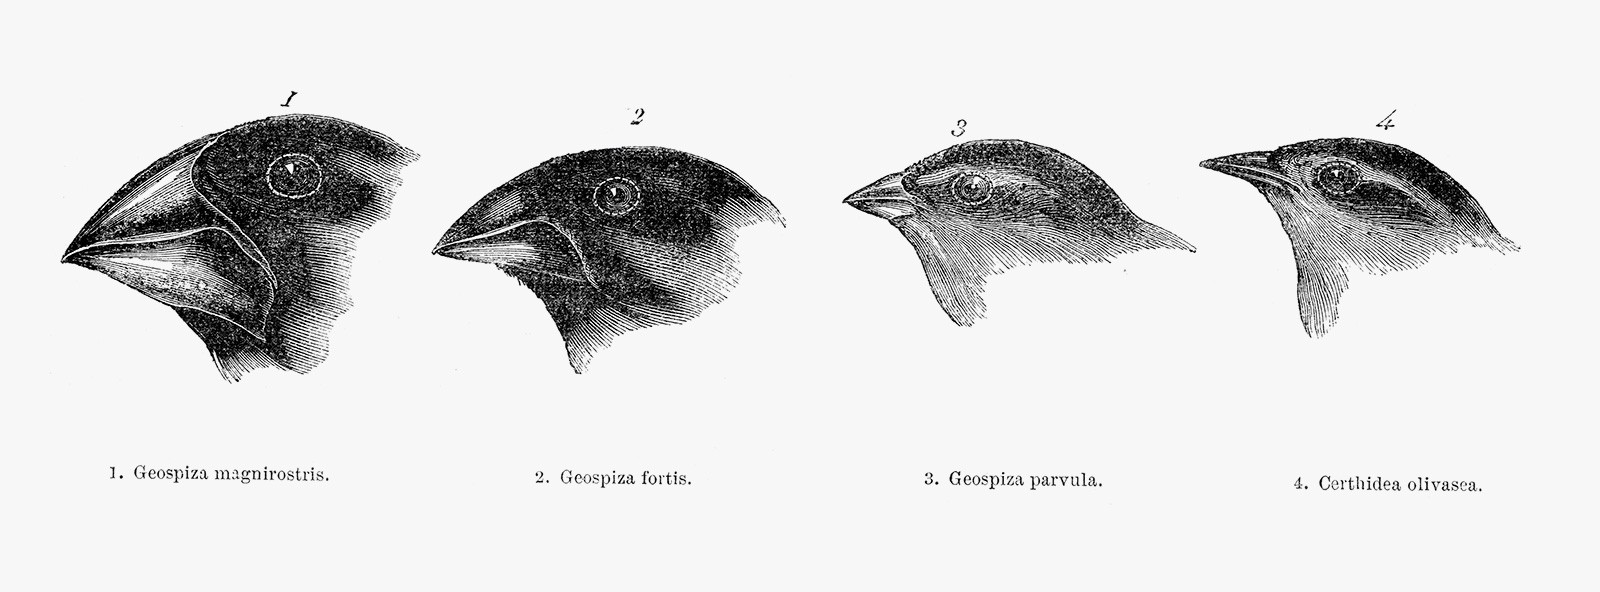
\includegraphics[width=\linewidth]{img/finchesFromGalapagos.jpeg}
  \caption{Finches from Galapagos archipelago extract od The Origin of species by C.Darwin .}\label{fig:finchesFromGalapagos}
  \endminipage\hfill
\end{figure}

%%%%%%%%%%%%%%%%%%%%%%%%%%%%%%%%%%%%%%%%%%%%%%%%%%%%%%%%%%%%%%%%%%%%%%%%%%%%
\subsection{Biologic evolution }\label{subsec:BioEvolv}

The Darwin theory of evolution was contested during long time until the confirmation by the progress of biologic sciences, especially with the genetic progress. The progress in this field was used to study the mechanism of the natural selection and evolution. One of the important progress and confirmation of the theory is by using the analyse of DNA code. DNA for DeoxyriboNucleic Acid contains all the useful informations growth, life and reproduction of life.   \\
The discovery of DNA code permits to confirm the genetic proximity between some species. Moreover the DNA permit to evaluate their evolution and code modification in the same species from different location and several generation gap. %voir eventuelement  l’évolution des petit lezar sur 20generation
Thanks to the genetic  and DNA the evolutionary process has been explained deeper and clearly. 



In the biology, every living element is composed by cellular. Inside each cellular  the DNA code is stocked. The DNA composes the chromosomes. The chromosomes have a central role in the definition of one individual and in the reproduction process (see the Fig \ref{fig:celTokrom}). \\
\begin{figure}[t!]
\center
\minipage{0.65\textwidth}
   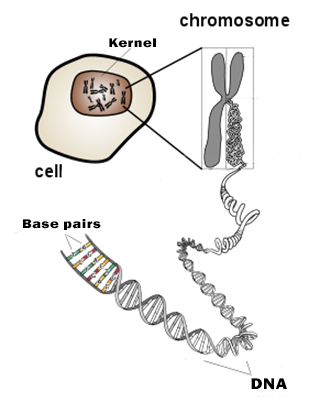
\includegraphics[width=\linewidth]{img/celTokromEN.png}
  \caption{Biologic representation, cell to chromosome until DNA.}\label{fig:celTokrom}
  \endminipage\hfill
\end{figure}
As has introduced earlier, the evolution is possible by a natural selection. The selection is done by survival and reproduction ability of the better individual. Better mean more adapted to this environment, like for the geospiza the size of the beaks depending than the size of the seed from his island.
In the island with the big seed  the geopiza with the small beaks was not the more adapted and have more difficulties to find food. This weakness makes the geopiza with the bigger beaks in better position to reproduce and the DNA of the individuals with biggest beak is transmitted to the next generation.\\
 The understanding of the reproduction mechanism in term of succession and transfer of the natural ability is primordial. It is explained in part by crossover in the cellular state.
 %sexual reproduction 
 \subparagraph{Sexual reproduction. }
The living element for example the geospiza use sexual reproduction. The sexual reproductions assume to merge  part of the chromosome form the two individuals to create their descendants. The selection is essential in order to keep the more adapted individuals of the species. \\ 
Among the reproduction mechanism the crossover and the mutation are the one with the bigger impact.
%% crossover
\subparagraph{Crossover. }
The crossover is the action of merging the chromosome of two individuals in order to have a new child.\\
It is an essential factor to preserve the individual ability of the geospiza. But the natural section and the crossover cannot be considered as the only useful element to evolve. 
%genome
\subparagraph{Genome}
The genome is a subset of the DNA code. Communally the DNA is cut in many thousand genome where each genome can represent a specified function or ability.  
%% mutatoin 
\subparagraph{Mutation. }
%The mutation is another essential element of the evolution process. 
Instead of the crossover which allows only the ability preservation from one generation to another, the mutation introduces some “anomalys”. The anomaly can become in some case a biologic advantage.
The mutation affects only rare chromosomes of the individual. The chromosomes affected are not fully mutated but only one or two genomes are affected. \\
%The genome is a subset of the DNA code. Communally the DNA is cut in many thousand genome where each genome can represent a specified function or ability.  
The mutation changes the little piece of DNA code to introduce variety in the genetic code by the small “anomaly”.\\
Most of the time the small mutations are not consequent for the individual but generation after generation the mutation can be preserved and spread in the population. \\  



The giraffe can be taken in example:\\
 In the arid environment, the giraffe with the longest neck has more chance to survive due to this empowered to find food. The giraffe with a neck a bit longer than the other, can become more attractive for the natural selection (in this case more food mean stronger and more attractive). The natural selection pushes the best individual to reproduce together and by the crossover mechanism conserves the small advantage given. The initial mutations given at few giraffe a longest neck and by the process of natural selection associate to the crossover allows this advantage form a small mutation to become the norm. Mutation by mutation and generation after generation the giraffe  saw the average length of their neck increased. Finally the actual giraffe is the result of a long and complex evolutionary process. \\ 
The mutation can also be the source of degenerate animals but in this case the natural selection  by the reproduction (and crossover) will not allow the preservation of the individual and thereby the mutated chromosome will disappear.\\ 
%%%%%%%%%%%%%%%%%%%%%%%%%%%%%%%%%%%%%%%%%%%%%%%%%%%%%%%%%%%%%%%%%%%%%%%%%%%%
%%%%%%%%%%%%%%%%%%%%%%%%%%%%%%%%%%%%%%%%%%%%%%%%%%%%%%%%%%%%%%%%%%%%%%%%%%%%
%%%%%%%%%%%%%%%%%%%%%%%%%%%%%%%%%%%%%%%%%%%%%%%%%%%%%%%%%%%%%%%%%%%%%%%%%%%%
\section{The evolutionary algorithms }
%\chapterintro
%The genetic and biology has given rise to the evolutionary algorithm family in computer science.  
\chapterintro*{T}he evolutionary algorithm (EA) is a big family of algorithms and they included many meta-heuristic used in the field of optimization and artificial intelligence.\\
 The evolutionary algorithm are inspired by the biologic mechanism for design meta-heuristics. The origin of the inspiration can be varied as  the genetic, insect work, animal behavior, … (see Table  \ref{tab:EAlist}). \\
 The biologic inspiration are not the only elements use to define the evolutionary algorithms. All the algorithms in this family are dedicate to optimize iteratively a population of solutions. 
 The EA family are not deterministic and use a randomised function in order to evolve. \\
 To summarize the EA have most of this attribute : 
\begin{description}
\item Bio inspired. 
\item Use random (not fully deterministic).
\item Based on population. 
\item Evolve a set of solutions to optimise a problem.
\end{description}
These characteristics are not the strict definition for all the EA. They are rather the most common element of the major part of the vast EA family. The EA family include several  sub-categories as in Table \ref{tab:EAlist}. In the following  part the EA is approach more in details,  first a brief historic of the EA. 
 
 
 \begin{table}
   \begin{tabular}{ | m{0.35\linewidth} | m{0.35\linewidth} |  }
     \hline
      \Emph{Inspiration or group}   & \Emph{Algorithm}    \tabularnewline \hline 
	  Based on memorization. & Neuroevolution				  	    \tabularnewline \cline{2-2}	
	  						 & 	Learning classifier system	 		\tabularnewline \hline 
	  Animal inspired and swarm algorithms & Particle swarm optimization (PSO) \tabularnewline \cline{2-2} 
	  				  		 & Bee colony 					  	    \tabularnewline \cline{2-2} 
	  				  		 & Ant colony 					 	    \tabularnewline \cline{2-2}  
	  				  		 & Mimetic algorithm			  	    \tabularnewline \cline{2-2}  
 							 & Shuffle frog					  	    \tabularnewline \hline  
	Swarm algorithms		 & Addaptatif dimensional search  	    \tabularnewline \cline{2-2}
							 & Gaussian adaptation					\tabularnewline  \cline{2-2}  
							 & Genetic Algorithm			  	    \tabularnewline \cline{2-2}
							 & simulated annealing			  	    \tabularnewline \hline  
	  Combinatorial      	 & Harmony search 				 	    \tabularnewline \hline
      Genetic  				 & Genetic programing 		 	  	  	\tabularnewline \cline{2-2}
      						 & Evolutionary programing 	  	  		\tabularnewline \cline{2-2}
      						 & Evolutionary strategies  		 	\tabularnewline \cline{2-2}
      						 & Evolutionary programing 	 	 	 	\tabularnewline \cline{2-2}
      						 & DarwinTunes 							\tabularnewline \cline{2-2}
      						 & Genetic Algorithm			  	    \tabularnewline \hline  
   \end{tabular} \caption{Liste of few basic EA.} \label{tab:EAlist}
 \end{table}
 %source : https://en.wikipedia.org/wiki/Category:Evolutionary_algorithms
%\begin{table}[!htb]
%\begin{tabular}{|l|l|l|l|l|l|}
%  \hline
%  \multicolumn{2}{|l|}{z=1 } &\multicolumn{2}{|c|}{GA}  & \multicolumn{2}{|c|}{PSO} \\  \hline
%  \multicolumn{2}{|c|}{ } & GT & NW & GT & NW\\ \hline
%  Room &  120x80 & 16 &20 & 16 & 20\\ \cline{2-6}
%     &  240x160 & 64 &70 & 64 & 70 \\ \hline
%  Room U &  120x80 & 12 &20 & 12 & 20\\ \hline
%  \multicolumn{2}{|l|}{z=2 } &\multicolumn{2}{|c|}{GA}  & \multicolumn{2}{|c|}{PSO} \\  \hline
% Room &  120x80 & 4 &10 & 4 & 10\\ \cline{2-6}
%     &  240x160 & 16 &20 & 16 & 20 \\ \hline
% Room L&  120x80 & 3 &10 & 3 & 10\\ \cline{2-6}
%     &  240x160 & 15 &20 & 15 & 20 \\ \hline
%\end{tabular}
%\caption{Design of experiment for comparing the efficiency of PSO and GA in different conditions.  (GT is Ground Truth and NW is Number of Waypoints).}\label{table:table1}
%\end{table}
%%%%%%%%%%%%%%%%%%%%%%%%%%%%%%%%%%%%%%%%%%%%%%%%%%%%%%%%%%%%%%%%%%%%%%%%%%%%%

%%%%%%%%%%%%%%%%%%%%%%%%%%%%%%%%%%%%%%%%%%%%%%%%%%%%%%%%%%%%%%%%%%%%%%%%%%%%%
\subsection{Historic}

The EA are relatively young  and do not have one fix origin. It is the result of more than a decade of research and improvement.
The premise of the EA can be the work of Robbins et al  \cite{184*robbins1951} in 1951. 
More commonly, the beginning of the EA are on the late 50s with the works of Bremermann \cite{185*bremermann1962}, Friedberg \cite{186*friedberg1958}, Box \cite{187*box1957}. They proposes different algorithms base on the evolving solutions to optimize a problem.\\ 
During almost the three next decade, the research had slowly progressed and they have remained rather unknown. Mostly due to the lower computation power at this time and also to some methodological short comings of
those early approaches. \\
Instead this difficulty, the fundamental works of Holland \cite{111*Holland1962}  and Fogel  has been essential to the progress and to popularize the EA. \\
As of 90s, due to the fast increasing computation power the EA became more popular and numerous new algorithms form EA family have been designed  as listed in the Table \ref{tab:EAlist}. The application of the EA in the engineering field (examples in \cite{10in182*alander1994}) and the multiplication of the conference around EA allowed the democratization of these family of algorithms.\\
The EA  has been profit of three main and independent methodologies; evolutionary programming, evolution strategies and genetic algorithms (GA). 

\begin{itemize}
\item The evolutionary programming, especially the work of Fogel is based on the finite state machine. The goal is to predict events based on the inputs, it is one of the premises of machine learning and classification.\\ %  sur les machine  a état fini (finit state machine ) ce sera les prémise de l'aprentisage

\item The evolution strategies, especially the work of  Rechenberg (\cite{rechenberg1965}), which propose a strategies based on deterministic selection and random mutation. The goal was to solve difficult experimental problem with discrete or continuous search space. \\ 
%strategies composé de mutation aléatoire et de slection deterministe  plutot destiner au espace continue et discret

\item The genetic algorithm is the most probably the most polyvalent and diversify of the EA (in terms of algorithm mechanisms). The GA propose an adaptive processes to optimize a solution. The detail of GA mechanism was explained precisely in the Section \ref{sec:GAdetail}.\\  
\end{itemize}

%finir le résumé  pour  evolutionary programing   et evolution strategie 
The GA has more particularly attracts the interest of the research with the work of Holland and  Goldberg. The popularity of the GA is most probably due to the increasing power of computation (in 80s, 90s) associate to fundamental progress and the numerous possible applications in the optimization field.

Since the late 90s the research of EA have been focused on the multi objective evolutionary algorithms MOEA   \cite{75*zhou2011, 114*Zhang2007, 140*soremekun2001}. %and MOEA/D = MOEA cut in subproblem



 
%%Wiki source 
%%Evolutionary programming was introduced by Lawrence J. Fogel in the US, while John Henry Holland called his method a genetic algorithm. In Germany Ingo Rechenberg and Hans-Paul Schwefel introduced evolution strategies.
%%a lire


%%%%%%%%%%%%%%%%%%%%%%%%%%%%%%%%%%%%%%%%%%%%%%%%%%%%%%%%%%%%%%%%%%%%%%%%%%%%
\subsection{General formulation}\label{sec:GeneralEAform}

 The EA is vast and many types of algorithms exist in this family, despite that a global formulation is proposed.\\
 Most of the EA have to optimize one or several problems using an iterative process to evolve towards a best solution. The EA can be formulated as the optimization of a parametres vector. Where each element of the vector ($\vec{x}$) is one input or a dimension to optimize. \begin{equation}
	\vec{x}= \{x_1,...x_n \} \in \omega
\end{equation}
Where $\omega$ is the search space of the problem, $n$ the number of dimension to optimize(or number of input). Each dimension of $\vec{x}$ must have a limited range (as $ \sum^{n}_{i=1} \sup x_i \leq x_i \leq \inf x_i$ ).  The search space represents all the possible solution of a problem. \\
In the case of the elements in the vector $\vec{x}$ are ordered, the search space even bigger. In this case, it is the product of each range of the vector.% ( as $ \prod^{n}_{i=1} \sup x_i \leq x_i \leq \inf x_i$ ). 
Where $||x_i||=\sup x_i -\inf x_i $ it is range size of  $x_i$ thus the size of the search is define as  $ \prod_{i=1}^{n} ||x_i||$. \\

Thus, the search space of the problem is defined by the boundary of each dimensions and the number of dimensions.  
%The association of each limitation for each dimension, define the search space of the problems( The boundary of the solution).
 Bigger is the search space, more the solution may be long to find in term of computation and power complexity.

 The goal of the EA family is to optimize inputs ($\vec{x}$ in order to have the best solution possible for the problem. Where the best solution is defined by a cost function depending than the input a vector $f(\vec{x})$. 
\begin{equation}
	\max f(\vec{x})\leq f(\vec{X})
\end{equation}
 Where  $\vec{X}$ is the global optimum solution. \\
 The cost function $f(\vec{x})$  is unique for each problem and have to be redesigned for  each problematic. 
Depending on the problem, the global solution is unknown and the best is to tends to this supposed global optimum solution. 
Optimize a solution $\vec{x}$ is not always enough to solve efficiently the problem. 
The solution proposed have to respect the constraint linked to the problem. The constraint can be various depending than the problem. As example one naive constraint is the boundary of the search space. To reach a set of $m$ constrain $E$ must be taken in consideration.
% But optimize a solution $\vec{x}$ depending on the fitness function is not enough to reach to the global optimized solution $\vec{X}$. To reach it a the set of $m$ constrain $E$ must be taken in consideration.
\begin{equation}
 \begin{split}
	\min (\sum^{m}_{j=1} e_j(\vec{x} ) )=E
    \\
	\max F(\vec{x}) \forall \vec{x} \in E 
  \end{split}
\end{equation}  
 $F$ is the final cost function, which include the constraints, to evaluate a solution $\vec{x}$ to optimize the problem. \\
The EA manage the optimization of the problem based on the cost function $F(\vec{x})$ by applying different meta-heuristic. 
The meta-heuristic use different methodologies to optimize an initial solution. The optimisation is more or less global depending than the method chosen. 
Mainly the optimization methods are based on the generate new sets of solutions. The new sets is made by evolving the previous sets of solutions. A set of solutions is also called population. %try to optimize an initial solutions based on the generation of a population of solutions. 
Where  a population is defined as $pop=\{\vec{x_1}, ...,\vec{x_p}  \}$ with $p$ is the number of individual in the population. 
%The EA are not obviously use in the convex problem 
The solution found by the EA is not mandatory the global optimum and for some type of problem (as Np-hard) it is impossible to confirm it. \\
The risk in this case is to try to optimize indefinitely. Instead to control the end of the optimization a stopping criteria  need to be taken in account.
%Instead to control the end of the optimization for do not indefinitely loop, a stopping criteria need to be taken in account. 

\subsection{Stopping criteria and convergence}
% \paragraph{Stoping criteria. // a deplacer dans le GA ou pour les algo de type GA PSO memetic ant}
 
The EA does not provide a solution to decide when it is necessary to stop the optimisation. 
To control the stopping criteria different solutions exist. The solutions proposed in the following part are mostly adapted to the algorithm like GA, PSO, mimetic and other EA working with a population to optimize.


% Therefore even if the global optimal solution is reached it is impossible to be assured of it. 
The EA algorithms are mostly efficient in the problems with many local minima. Due to numbers and size of the local minima it can be difficult to ensure if a solution is the best or more exactly the global optimum. 
To know if the global optimal is reached, the method must be sure that no other solution can be better. Therefore the solution found must be always exactly the same or equivalent in term of cost. The optimisation process must be reproducible (same input gives the same output).\\
 Only the deterministic method can insure to have a global optimum solution as a convex problem. The convex problem has only one global optimal and no local minima. \\% Using a algorithm from the EA family do not authorize such insurance due to the randomness effect proper to the EA.\\ %manly due to the impossibility to reproduce every time the same result in the same condition due to the randomness effect proper to the EA family.
  In this case, the EA looking for the better solution possible (not the optimum). That can be in some case the same than the global optimum but because of the uncertainty is impossible to call global optimal it is just the better solution founded.  
 
% methode non deterministe donc imponsible de connaitre la solution optimal donc commen sarrété.
%How to know if a solution is the better solution and related to
%In many case the optimal solution cannot be reach and a stopping criteria should be defined. Manly 3 possible way are communally use.

Based on that, how  determine when is time to stop the optimisation with EA. At some point is useless to continue the optimization (best solution founded or lock in some deep local optimum) and a stopping criteria should be defined.\\ 
Three possible way are communally used:\\
\begin{itemize}
\item The first method (called fix time criterion), is to stop the optimization after a fix numbers of iteration or time limit. The limit is measured in term of time computing, also the numbers of iteration must be fixed by the user. The interest of this method is mainly to control the computation time for the problem requiring a solution in a determined time (as a real time). The risk of this method is to stop the optimization before to have an efficient solution. \\
This solution can be mixed with other method to reduce the number of useless iteration.% for control the case where the  other method are too long.  

\item The second method (called update criterion), is to stop the optimization (before the convergence) if no better solution is found after a predefined number of iteration. This criteria can be useful for the complex problem or if many solution can have the same quality. 
The advantage of this solution is to can stop before the convergence with a close solution. The inconvenient is to stop too early, in the beginning of the optimisation due to a good initial solution.   \\
To use this stopping criterion a correct number of iteration has to  be selected. 
The number of iterations  must be sufficient to give time when the meta-heuristic is lock local minima. 
A long time lock in local minima may append mostly at the early time of the optimisation due to the too good initialisation or in the late optimisation time (when the solution is already well optimized).\\
 In contrary a stopping criterion with a too big number of iteration became use less. In the worst case, the convergence point will be reached  before the too big number of iterations.
%si la meilieur solution est pas ammélioré 

\item The third method, (convergence criterion), is to stop the optimization by waiting the convergence point. The convergence is reach when the actual population is composed by a set of solutions identical. That means the same solution has been founded by all the individuals of the population. \\
 The best solution found push the other to evolve in the same direction, by contagion all the individual of the population evolves to reach the convergence point. \\ 
 This solution found during the optimisation process is supposed to be the better. In this case, the population has been converging to an optimized solution. At least no better solution can be found during this optimization.\\
\end{itemize}
These 3 criteria are the more commune, but depending the problem other criteria can be found with more or less a priori on the problem.\\

 Moreover the stopping criteria presented can be a combined to have an efficient and flexible solution as  in the following example :\\
The mixed stopping criteria has to combine a fix time criteria and the update criteria.
The advantage of the fix time criteria is to avoid the case of an almost infinite optimisation loop append, due to an impossible convergence.%(which leave a good room for manoeuvre to reach the convergence), 
\\ %The fix time criteria is fix widely to leave the manoeuvre to reach the convergence. \\ 
Combined with the update criteria the other advantage is to can stop the optimisation before the convergence and before to reach the time criteria limit.\\
The combination of these stopping criteria assures to have always a solution optimize in a reasonable time (fast, efficient and time predictable for the worst case). 

% Tout la population a la meme solution
 
%%%%%%%%%%%%%%%%%%%%%%%%%%%%%%%%%%%%%%%%%%%%%%%%%%%%%%%%%%%%%%%%%%%%%%%%%%%%%
%\subsubsection{ Relation enter Darwin et EA  }
%
%%%%%%%%%%%%%%%%%%%%%%%%%%%%%%%%%%%%%%%%%%%%%%%%%%%%%%%%%%%%%%%%%%%%%%%%%%%%%
%\subsubsection{ Historique des EA   }



\section{Genetic algorithms} \label{sec:GAdetail}
Among the evolutionary algorithms one of those was very close to the Darwin theory by reusing the operating principle of natural selection and was also based on the genetic with the influence of the crossover and mutation (see section \ref{subsec:BioEvolv}). This algorithm is called Genetic Algorithm (GA) and was introduced for the first time by Holland in 1962 \citep{111*holland1962}. \\
The genetic algorithm (GA) is from the EA family but is also one of the fundamental algorithms of the EA.
The GA became popular at the late 80s and early 90s, particularly with Goldberg works \cite{112*goldberg1989}. Many details were redefined and explored in the knowledge of genetics to have a huge set-up and operator available for the GA.


   
%\subsection{Ga in detail}  

%After have seen in the previous part  the origin and some reference about the evolution of the GA.
In this section, the GA will be present with more interesting advance and set-up. 
The following section will try to list the more interesting aspects of the GA mechanisms. 

% It will not be a list of all the different implementations and mechanism, rather a detailed explanation that also gives the different optimization lists already explored or the more usual ones.  
 
 The explanation will be separated in 6 sections with:
\begin{itemize}
\item [1)] 	chromosome representation 
\item [2)]	population size 
\item [3)]	cost function 
\item [4)]	selection mode 
\item [5)]	operator 
\item [6)]	setting 

\end{itemize} 

Before to begin, it is important to remember the GA is an algorithm used to optimize a solution while still on a non-deterministic initiative and therefore can not give the certitude to have the optimal solution. 

\subsection{Chromosomes} \label{par:Chromosomes}
As in the Biologic field the chromosomes contain the properties (with the genomes and DNA) of the individual.
A primordial issue when you want to optimize a problem involving the GA is to define properly the chromosomes role, for that different aspects must be taken into account.\\

The first aspect is related to the problem himself. The chromosome is used to design the problem and it has to represent a solution. To do so, it is important to know the problem and identify clearly what parties of the problem need to be optimized and what is the range of the research area. \\
Depending on that the coding can be direct or indirect.
\begin{itemize}
\item The direct coding is code with the genomes corresponding to the elements of the solution. Using the direct coding may simplify the output of the optimization by returning it back to an element directly proper to use.
\item  In Contrary, the indirect coding, it is not directly proper to use and need conversion to be used. One example of indirect coding is the willingness to introduce redundant genome inside each chromosomes.  The conversion must be done by a heuristic. The interest of the method is to be able  to make a strong constraint adapted to the problem as \cite{121*ronald1997,131*walters1995}  where it is used to solve a complex scheduling problem with many constraints. 
\end{itemize} 
 Inside this article the interest between the direct and indirect coding are presented.  \\ %indirect ex metre de la redondence dans le chromosome
The diverse aspects of the problem should be clearly defined before the element makes up the chromosome, like  the number of dimension to optimize, the boundary of each dimensions and the importance of the dimension order. 
%!!!a finir verifier et surmen réecrire!!!!
When the chromosome is defined the second phase is to choose the best coding solution. Many solutions exist to encode the chromosome like presented in \cite{131*walters1995} and \cite{123*owais2008}   but among the coding solution, 4 main categories can be considered as  basic coding type,  which are the combinatory coding, binary, the real (also alphabet) and tree coding.

\subparagraph*{Binary Coding}(\cite{73*wright1991, 95*miller1995,97*goldberg1985,123*owais2008, 131*walters1995})  
\\The binary coding offers to format the chromosomes as a bit string in which every genome of the chromosome can be covert on pack of bit with can have only 2 value 0 or 1. This coding method was studied since the beginning of the GA by Goldberg et al  \cite{97*goldberg1985} and also used in other EA like PSO in \cite{87*morsly2012}. The binary coding is more efficient in the small search space or when the size of the chromosome is not too long. The advantage of the binary coding is the possibility to introduce lot of variety during the process of optimization \cite{73*wright1991}. The variety is traditionally from the mutation but in the case of the binary coding the crossover introduce variety by the potential split of the genome in 2 pack of bit.
\\
\subparagraph*{The combinatory }(\cite{ 80*serpell2010,110*eiben2003} )
\\The combinatory coding is commonly applied in some specific problems where the goal is to order all the element. In this case, the position of the genome in the chromosome is primordial as in \cite{ 110*eiben2003}. It is characteristically used to the problem as TSP \cite{80*serpell2010} (Travelling salesman problem).  When the combinatory coding is used for problem the aim is to optimize the order the element of the chromosome. With a combinatory coding the each chromosome already has all genome of the answer. An example, the TSP the aim is to order various cities (in the problem of TSP every genome represents a city) and all the possible cities are included in the initial solution (chromosome). In this case, the problem is to optimize the combination of the element composed by the initial solution. 
One evolution of the combinatory traditional coding is to can add and remove some genome, that obviously affect the size of the chromosome, for example  when the goal is to find the shortest distance in the tree \cite{113*mais2010}. \\

\subparagraph*{Real Coding }(\cite{ 73*wright1991, 123*owais2008,131*walters1995})   
\\Real coding or integer coding is considering every genome of the chromosome as a number to optimize. This number can be a real or an integer and may have an infinity of possibilities in the negative or positive. In fact, the value does not have an infinity of possibilities because the constraint by the computer and limits of the problem itself too (size of the search space). This coding is used when the search space is large and also can be efficient when many dimensions need to be optimized. But most of the time a special attention should be put to the operator, because in many cases the operator may be adapted or redesigned depending on the problem such as in \cite{68*muhlenbein1989},  which the operators are adapted to look for close neighbours.\\
\subparagraph*{Tree coding }(\cite{ 113*mais2010, 123*owais2008, 131*walters1995})   
The tree coding use the tree representation to take care of the hierarchy but this method is not really popular and not flexible to any case. The advantage of tree coding is this ability to go farer then a combinatory representation.  An example in \cite{131*walters1995}, the tree coding is used with the GA to optimize new network telephone or gas/ water pipeline where the relation between the element are primordial. In \cite{131*walters1995} present the interest of tree coding for  the intrusion detection system. 
\\
The 4 coding method presented are not the only potential coding, there are the more commune and the roots of other coding   and many other have been developed and studied with direct or indirect coding to feet  with specific problem. Thereby in the literature a survey are dedicated to the encoding chromosome for the GA \cite{121*ronald1997}. The survey \cite{121*ronald1997} propose to explain and find a robust coding usable depending on the problems. 
\\

%\begin{table}
%   \begin{tabular}{ | m{0.30\linewidth} | m{0.65\linewidth} |  }
%     \hline
%     \Emph{ Reference}   & \Emph{Chromosomes interest}    \tabularnewline \hline 
%	  Walters et al 1995 \cite{131*WALTERS1995} & Use the GA for pipeline position optimization with a tree coding and a talk about the choice of the coding compared to the binary coding and alphabet coding.  				  	    \tabularnewline \hline 
%	  						 & 	Learning classification		 		\tabularnewline \hline 
%      Genetic  []			 & Genetic programing 		 	  	  	\tabularnewline \cline{2-2}
%      						 & Evolutionary programing 	  	  		\tabularnewline \cline{2-2}
%      						 &	Evolutionary strategies  	  	 	\tabularnewline \cline{2-2}
%      						 &	Evolutionary programing 	 	  	\tabularnewline \cline{2-2}
%      						 &  Genetic Algorithm			  	    \tabularnewline \hline  
%   \end{tabular} \caption{Liste of few basic EA } \label{tab:EAlist2}
% \end{table}
%The variety is introduced due to the cutting pack of bit during the crossover. 



%[131*] codage par tree of GA codage par lettre alphabétique au lieux du binaire. 
%[121*] survey codage indirecte avec redondence 
%[123*] codage binaire and tree codage .  Use GA for security   ralk about the encoding chromosome  wihe  binary  permutaiton  real tree

%Parties détailler 
%1)	Comment représenter un Chromosome (individual) \\ 
%-	Codage Binaire (utilisé au début)
%-	Codage Réel  (plus adapté au problème  de variable  continue) 
%-	Codage combinatoires (pour les problèmes combinatoires) (à vérifier) 
%-	Tree coding
%
%2)	Fonction de cout :\\
%-	Importance de la fonction et universalité (même fonction pour tout les metaH)
%-	Multi objectif 
%-	Constraints (inside the cost function)
%-	Optimisation  and time computation 
%3)	Population \\
%-	population initiale  
%-	la rapidité de convergence  et variété 
%-	 taille de la population
%4)	Mode Sélection :\\
%-	Le rôle de la sélection 
%-	Elitiste selection
%o	Fonctionnent 
%o	Adaptation pour du MOEA
%-	Roulette wheel selection 
%-	Tournament selection 
%o	Fonctionnent 
%o	Taille de la poule 
%
%5)	Operateur  et leur fonctionnement\\
%-	Cross over
%-	Mutation
%-	Rate of operateur
%
%6)	Paramétrage : \\
%-	Liste de paramètre
%-	Leur inter relation 
%-	Configuration par test 




%%%%%%%%%%%%%%%%%%%%%%%%%%%%%%%%%%%%%%%%%%%%%%%%%%%%%%%%%%%%%%%%%%%%%%%%%%%%
\subsection{Cost function }\label{sec:CostFunctionGA}
	The cost function or some time called fitness function has an essential role in the optimization process.  The aim of this function is tantamount to quantify the quality of one solution. This point is primary to the GA and in most of the optimization process using meta-heuristic. The cost Function is an compass the meta-heuristic during the  optimisation. 
	The cost function is dependent then the problem and should be design or redesign depending on each specific  problem. Once the cost function is designed for a problem they can be used to test different other algorithms of optimisation with requires also a cost function. 
	Because the cost function is exactly the same that becomes easier to compare the results from different algorithms as is discussed in \cite{79*franccois2001} and also in the chapter \ref{sec:GAvsPSO}.%[GA VS PSO 5.2 ] 
	Once conceived the cost function is considered as a black box by the optimization algorithm and encloses most of the complexity of the problem. Obviously if the cost function is not designed correctly with all the constraints and the objective, the optimization will fail.\\

\paragraph*{Multi objectives}
The cost functions are traditionally made-up for  problems with only one objective, but in the recent years several solutions have been adapted for multi objective. The goal is to optimize a problem with few sub-objectives included. These sub-objectives can be at some point contradictory and a trade off must be done during the optimisation process, based on the rating made by the cost function. \\
 The cost function for multi objective problem (MOP) is discussed in the survey of Zhou et al \cite{75*zhou2011}. In Zhou et al \cite{75*zhou2011} one of the ways to solve the MOP is to adapt a classic mono objective algorithm in multi by customizing the cost function. The customization of the cost function propose a way to evaluate a solution not depending than one objective but with all of them combined in the same function instead of several cost function. 
 Also other solutions are discussed in \cite{75*zhou2011} like using coefficients for order the objective priority or by reducing the problem into several sub-problems. \\ %  reference pas naive car  ce sons celle qui seron utiliser par la suite

\paragraph*{Constraints}
The goal is to satisfy the objective(s) while taking into account the constraints. Consequently the cost function has to take care and integrate the constraints. 
 Previously in the chromosome (\ref{par:Chromosomes}) the strong constraint was established by the coding, especially by imposing limits in the real coding or using indirect coding, but it is feasible to impose some soft constraints in addition to the system by adding the rule in cost function. The rule corresponding to the constraint is helping the optimization to do the good choice not by imposing strong constraint but by affecting "bad points" or "good points" depending on the constraints. \\
 The soft constraints can appear a bit useless, but there can be a good trade-off between two contradictory objectives and some other strong constraint, also a soft constraint can be easier to implement and faster in term of time computation compared than a hard constraint.  

\paragraph*{Optimisation and time computation}

The cost function should be designed carefully and have to pay special attention to the time computing. Indeed the hight frequency call of the function may generate some heavy slowdown. \\
The cost function has a special importance in the optimization process to  the rating of all the individuals at every generation. If we consider a GA with 100 individuals (it is a common number of individuals  not to much and  generally enough ) and a convergence after 100 generation (it is good minimum in order to avoid a premature convergence), in this case the cost function will be call at minima 10 000 time. Due  to this important factor it is primordial to carefully design the cost function as is specified in \cite{70*arabas1994}.\\
It is common to have several thousands or billion calls of the cost function during the optimisation process.
  Hence the importance to have a function timeliness and economic in resource. \\
Even the cost of this function must be the most accurate, in some cases like in \cite{95*miller1995}, a complex calculation or noise can affect the reliability of the cost function which will be impacted on the quality of optimized solution but despite the noise and the weakness of the cost function the GA can optimize and give a solution. But it is advisable to have a function accurate and reliable as possible to have an efficient solution.\\
 To conclude with, the importance of the cost function is a major piece of the GA and the choice of the design of cost function associate to the chromosome representation will affect the result but also the setup of the GA and can generate some lock. \\

	
%%%%%%%%%%%%%%%%%%%%%%%%%%%%%%%%%%%%%%%%%%%%%%%%%%%%%%%%%%%%%%%%%%%%%%%%%%%%
\subsection{Population }\label{sec:Population}
The population gathers a number N of solutions (or individuals) from the same generation. The individual can be represented into one or  more chromosomes(instead to have redundancy as in \cite{ 121*ronald1997}). Commonly each individual is composed by one chromosome. Therefore the two terms are regularly inverted in the literature.\\
At every generation most or all the population is renewed (by using the selection and operator). Indeed the population can have an effect on the convergence and the result of the EA and different strategy or set up exist. About the population 2 main points need to be studied : the first is the initial population and the 2nd is the size of the population.  
\subparagraph{Initialisation of the population}\label{sec:initPOP}
Initialization of the population is one of the fundamental questions may affect the convergence of the problems. There are mainly 2 common proposed solutions with one using the full random generation or  using efficient and already approved heuristic.\\

 The method is based on heuristic involved a perfect knowledge  of the problem and can not be applied  for all the problem. The advantage of using heuristic, it can give very good starting individuals at the beginning the optimizations and also used the heuristic may give a solution more respectful of the constraint of the problem, obtusely if the problem include many constraints hard to satisfy. \\
Although this advantage of using a heuristic to find the 1st generation of the population, can become a handicap and push the GA in the direction of the potential local minima. Indeed using one heuristic to build the first generation can have a population too similar with not enough variety. The variety is essential to run through all the searched space and allows do not converge too fast in a local minima (see \citep{64*matsui1999}).\\

If using a heuristic to build the initial population is not always the good solution one other solution more versatile is to use the randomness to find initial population. The  randomness generates each individual randomly in the search space. One of the advantages is the individual can be well distributed around the search space to cover most of it  if the size of the population is big enough. 
The random  distribution permits the algorithm  to cover a wide part of the search space quickly during the first generation and the spreading of the population is a good source of variety.
The random initialisation is commonly used and less often the heuristic solution.

To initialise the population, the third method is to combine the full random with the one based on heuristic. 
In this case, for examples a random solution is applied before, the heuristic is used to refine the initial solution. Otherwise different heuristics are used randomly to generate all individuals of  1st the population. Other combination are possible  see \cite{113*mais2010} for more detailed see.

\subparagraph{Population size}
An other key point is to consider the size  of the population. The size of the population and this effect on the convergence are studies in many articles \cite{64*matsui1999,70*arabas1994,71*grefenstette1986,77*shi2005,97*goldberg1985,109*cerf1995}. 
The first point is to find the appropriated size depending on the problem. Indeed if the size of the population is too small the variety of the population can be too short and the algorithm can converge too fast \cite{70*arabas1994}, instead if the population is too large the waiting time may become too long.  
Like that, chose the appropriate the size of the population is not trivial at all. To find the best size of a static population only one way, is to do several experiments and compare the results, like did it in \cite{71*grefenstette1986}.

 The population can also be adapted dynamically or auto-adapt the size of the population during the optimization. Commonly the number individuals in the population need to be important during the first generation but close to the convergence the population can be reduced for win time.
  In \cite{133*schwefel1984}, the size is fixed by probability. It can also be fixed by a linear equation or even more complex, in function of the progress of the cost function and the variety of solution see in \cite{70*arabas1994}. The population have an important part in the convergence computation, depending on if the size of the population is static, dynamic or auto adapted the convergence can be faster with more or less quality for the solution. The convergence is studied in the \cite{109*cerf1995}. But the convergence is not only link by the population size but also the selection, the coding and the operator choice are an important aspect of the GA like is showed in \cite{71*grefenstette1986,77*shi2005}.  



%	\paragraph*{Population initialisation }
%	\paragraph*{Speed convergence and variety}
%	\paragraph*{Population size}
%%%%%%%%%%%%%%%%%%%%%%%%%%%%%%%%%%%%%%%%%%%%%%%%%%%%%%%%%%%%%%%%%%%%%%%%%%%%
\subsection{Selection mode  }

 What is the selection mode? \\
 The selection mode is  the method  used to select in a population the individuals the most able to reproduce. It is an important key point corresponding to the natural selection in the Darwin theories. \\
The choice of the selection mode is primordial and affect greatly the quality and the speed of the optimisation process. This choice needs to be done depending than the problem. A selection mode applied on a specific problem  can be efficient (in term of answer quality and time convergence)  but  the same  selection mode applied on  a completely different problem can be inefficient for it.  The selection mode must be selected or adapted for each kind of problem. To choose the selection mode no magic  bullet, the testing of different method has to be done.\\
One of the objective of the selection mode is to keep enough variety in the population to avoid an untimely  convergence. Also too much variety in the population and especially not a the beginning may artificially delaying the convergence. A good selection mode has to trade off between too elitist selection (not enough variety) and a too permissive selection (too much variety). \\
A multitude of selection mode has been developed during the time (few of them have been listed in \cite{123*owais2008}). Make a choice among this wide list of possibility is difficult. The selection mode among the most common  or representative is  presented:    \\

\subparagraph{Elitist selection}
-	The elitist selection is more like a subgroup of selection mode. His particularity is to use a deterministic way to selected the best individual depending of the cost function the best or some of the best are selected directly for the next generation like that the best individual are preserved and no risk  to lose one good individual during the crossover, mutation and other operation. The few best individuals selected are used to engender a new generation.
  This subgroup of selection is studies as in \cite{69*deb2000,64*matsui1999}  to estimate the efficiency of convergence using this selection mode or in \cite{140*soremekun2001} applied in the multi-objective problem. It is appeared on this article the elitist selection is efficient, converge quickly and the best individual founded are preserved  for the next generation. But unseemly it may sometime converged prematurely most of the time because of this difficulty to keep enough variety wish this selection mode for that some of the elitist selection have been customized to try to preserve the variety. \\
	
\subparagraph{The roulette wheel}
-	The roulette wheel selection is at the same time one of the older selection mode used since 1989 but also one of most inspiring.  The roulette wheel  gives many methods inspired by this one like for example remainder stochastic sampling in  \cite{138*whitley1994}. The roulette wheel selection had a basic operating. Every chromosome is represented in the wheel and the size of the wedge are depended them the quality of the chromosome. This quality is computed from the fitness function.  With this technique, the chromosome with the best fitness function has the most luck (but not necessarily) to be selected. 
Once the wheel was built by the random sampling can begin to select the new individual of the generation.  The wheel turns until all the individuals are selected.  
This method helps the better chromosomes to be more represented in the next generation but also accepted to have some time more or less bad individual conserve for keeping the variety. More the GA work more the size on the wheel of the best solution will increase and help to converge. \\

\subparagraph{Tournament selection}
-	Tournament selection is one of the most used  in this last decade. It is working as a tournament. 
The first step is to create few pools with all the individuals of the actual generation. The pools are randomly create.
 When the pools are created, the tournament can begin and the best chromosome of each pool (depending to the cost function) are selected for build the next generation, with the other winner. 
 This selection by randomly build the pool, help some not good individual to continue but the best chromosomes are always used to build the next generation. The tournament selection is very efficient to keep diversity and also give a chance to have a fast convergence as is explain in \cite{64*matsui1999}. \\ 
 Obviously the size of the pool has a really big influence on the convergence as is studied in ,\cite{64*matsui1999,95*miller1995}. The conclusion of these papers about the pool size  is, bigger is  the pool (4 or 5 individuals) less diversity is kipped and the convergence goes faster, and can finish lock in a locale minima due to a premature convergence.
  In the other side the small pool (2 chromosomes) keeps the variety but the convergence can be slower. 
  Finally the size of the pool is also one other parameter to take care and the size of the pool is also strongly linked to the population size.
Among the selection mode presented tournament selection is one of the most efficient  for manage the  variety and that explain this  wide popularity to solve an engineering problem. \\ 

\begin{figure}[t!]
\minipage{0.85\textwidth}
   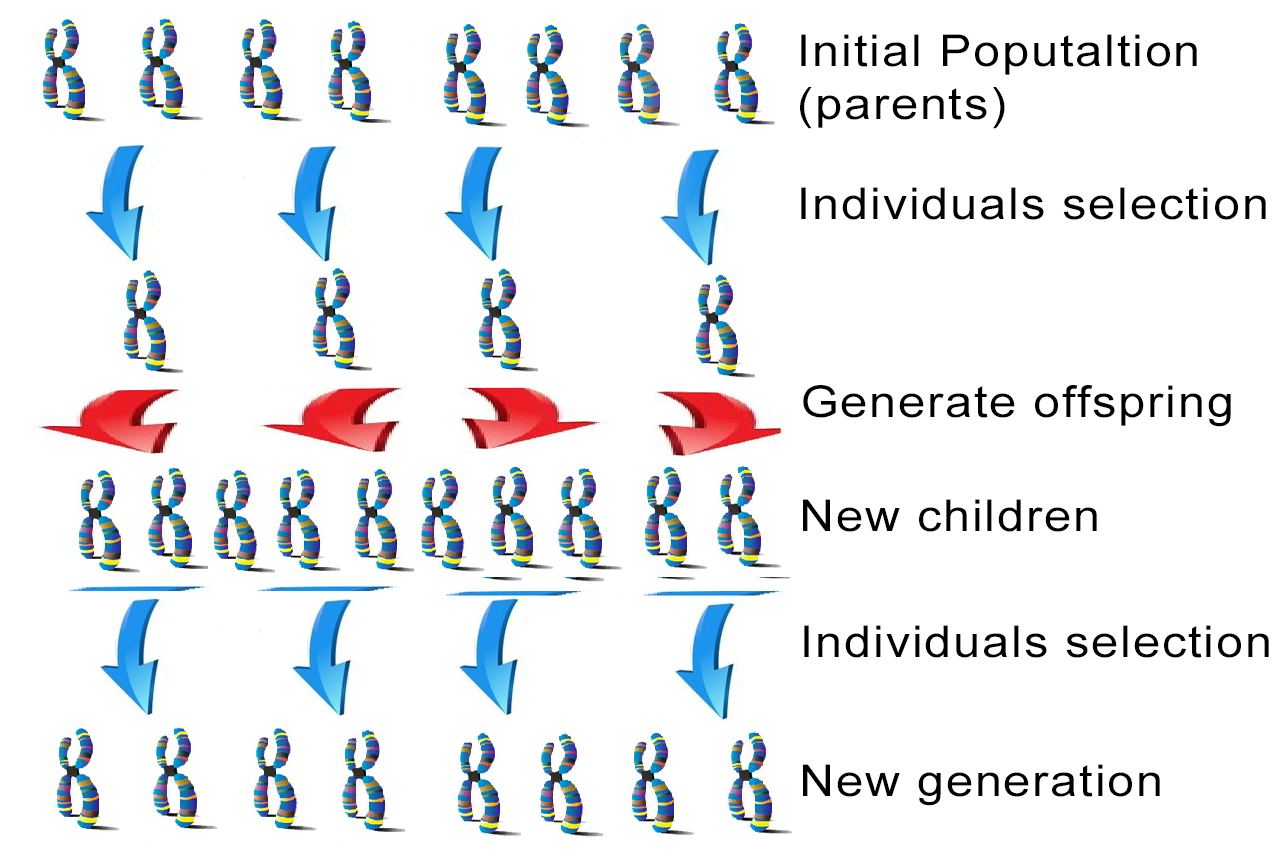
\includegraphics[width=\linewidth]{img/GA2selections.png}
  \caption{The 2  time for  the selection mode with the GA  mechanisme.}\label{fig:GA2selections}
  \endminipage\hfill
\end{figure}
The last element to consider about the selection mode is when it is the more appropriate to use it? 
Indeed  the selection of the individual may intervene at 2 occasions (see figure \ref{fig:GA2selections}).  The first  the more conventional is  to select the parent  able to reproduce. The second is to select the children good enough for be part of the next generation. The interest of this is to be able to generate new children until the selection criteria are rich in order to have a population with acceptable children in sufficient quantity (This method is more efficient on the problem with lot of hard constraint). 


 

%idée 1 :  quesque le mode de selection  ...  
%			 c'est la method qui va etre utilisé pour choisire les individue qui pouron ce reprorduire.
%idée 3 le choix de ql selection est la plus aproprier
%			   le mode de selection impacte la qualité et la vitesse de la réponce 
%			   le mode choisie et fait en contion du problem a résoudre (pas de recette miracle) 
%
%idée 4  le mode de selection doit gardée une certaine variété  pour  avoir une convergence 
%			mais pas trop.
%			 
%idée 2  l'importantce de la selection 
%			 une population trop élitiste peu convergé prématuréméne 
%			  une selection trop peu restrictive peu empéché la convergence et l'optimisation

%idée 5  une multitude de mode de selection existe 123*
%
%idée 7 les modes de selection les plus comu et représentatif  
%
%idée6   la seleciton peut etre fait a plusier momen  64*
%			selection des parent
%			selection parmis les potentiel enfant les ql vous sourvivre 
	


%The selection mode have aim to pick-up the individual (or chromosome) the most interesting of the actual generation for build the next one.
% The individual chosen can be called parent, they reproduce to build the next generation.
%One of the difficult point is to understand who the more interesting individuals are from the actual generation. To this choice is essential because depending to the choice the quality of the answer and the convergence will be affect. 
%
%Among the goals of the selector is keep the variety and help to converge but for that is primordial to know the difference between the selections modes. Many mode was designed [123]* or adapted but some of they are more used and studied. Also the selection can be done at different time.  First for select the parent or after the crossover mutation and other operator for select the best children or even use both like is showed in [64]*.


%le role de la  selection 
%	\paragraph*{Elitist selection}
%	\paragraph*{Roulette wheel selection}
%	\paragraph*{Tournament selection}
%		\subparagraph{fonctionment}
%		\subparagraph{pool size}
%	
%%%%%%%%%%%%%%%%%%%%%%%%%%%%%%%%%%%%%%%%%%%%%%%%%%%%%%%%%%%%%%%%%%%%%%%%%%%
\subsection{Operators }


The operator have to aim the design of the next generation by generate the offspring. 
Once the parent able to the reproduction were selected (using the selection mode saw previously) it is time to engender a new children.
The techniques, to create a new population are numerous. Among them the more common  are the heritage (or selection), random generation, the crossover and mutation. 

\subparagraph{heritage or selection:}
The heritage or also called selection is a simple copy of the best parents to the next generation with no modification. This operator is commonly used to keep the best individual in order to do not lose the best solution if no upgrade is made by the other children. Indeed the other operator may propose degenerated children with is some time worst then their parents and the heritage  permit to conserve as is the individuals.
\\
The crossover and mutation have a more interesting mechanism. They are also the basis of many other customized operators and the understanding of the basic crossover and mutation required to use it.
 
 
\subparagraph{Crossover:} 

The crossover operator is directly inspired by the biologies. As 2 mammals reproduce to have progeny. Half of the genetic material of the two parents are used to create a child.
The crossover operator is mixing 2 individuals to create a new child. The aim of this is to merge 2 workable solutions to have one other solution potentially a bit better. To merge the 2 individuals it is existing many way like studied in \cite{113*mais2010}.
 
 \subparagraph{Mutation}
The mutation operator have to aim to add diversity by mutate some random allele of the chromosome. This mutation must be randomly choose and are useful to keep the diversity of the population. As the crossover different mutation are existing \cite{113*mais2010}. The mutation mechanism affect only rare genome in all the population. The genome mutated is randomly selected and the is will be based on random. 

\subparagraph*{Customized operators}
This 2 principals operators need to be choose carefully and in most of the case redesigned.
The redesign of the operator is essential in many occasion.
One of the first reason to redesign part of the operator is to fit well to the problem. A example is the mutation redesigned to explore the search space with a logic of close neighbour as in \cite{68*muhlenbein1989}.\\
The second reason is link to the chromosome coding. Depending on the chromosome coding chosen (binary, combinatorics, real, ...) the operator have to be adapted. An example is to modify the mutation and crossover to preserve the genomes in the real coding. The same operator can not be used for combinatoric coding or binary.\\
The third is more rare but in some case the operator have to be adapted depending on the selection mode chosen. An example is  given in  \cite{65*thierens1994} with the crossover and the mutation for a elitist selection. \\
Also one other reason to redesign the operators is to have operator fitting  to some of the hard constraint to the problem. In order to have operator able to create children respectful to some hard constraint of the problems.


%redesign some operateur (mostly  crossover  and Mutation
%idee 1 : operateur redesigne to fit the problem
%idee 2 : operateur redesigne to fit the chromosome coding (pour ne pas coupe des gene  ) 
%idee 3 : operateur doive etre adapté au mode de selection  comme le crossover  avec une selection elitiste 65*
%idee 4 : redesign a operateur  pour respecter certaine des hard constraint
% In many case the crossover need to be designed or redesigned depending to the problem. 
% In order to have an adapted crossover  the chromosome coding is primordial. Depending then if the chromosome coding is binary,real or other the the crossover must be redesigned to respect the it. Also the  crossover should be redesigned  
% Also the crossover work differently if the chromosome are code as binary or real for example and the crossover should redesign depending to the problem, the coding and some time for some specific selections like for elitist recombination [65]*. Redesigned the crossover can be useful to have crossover respect the genome or to can directly have an operator generate a solution that respect some of the hard constraint. 
% Mutation custom
%  and some of them are specific to the coding of the chromosome because like the precedent operator presented the  coding  affect the implementation of the mutation and may redesigned depending to the problems and also be redesigned do explore the search space with a logic of close neibourgh  like in [68]*.\\


\subparagraph{Operators rate}
 An other important element to take in consideration after the choice of the operator and their implementation is  rate of each of then. 
The rate of an operator correspond to the usage percentage of the operator on the chromosome, higher the rate is,  more this operator will be used at each generation generation. 
In the mutation the rate can be globally understood as a chance to one an genome to be muted. 
Finding the  best rate for every operators became a real challenge. The best solution to find the appropriate  operators and their associate rate for a specific problem no other choice to try the couple combination of operators with different rate like in \cite{73*wright1991,71*grefenstette1986,133*schwefel1984}.\\

 To conclude on the operators, they are an important factor to evolve generation after generation.  The operator have to keep the diversity  in order to have an efficient converge (not premature and not to late). The question of the diversity introduce by the operator was been studied in  \cite{80*serpell2010,95*miller1995} \cite{113*mais2010}. 
 It is appearing one good static configuration to keep diversity \cite{64*matsui1999} of chromosome is to have crossover mutation with height rate of crossover and small rate of mutation. 
But the rate of the operator can be adapted depending on the searched space, the convergence and other element. Some research was done on adapted the dynamically the rate of the operator depending too many external factor or using probability like is discussed in  \cite{110*eiben2003,133*schwefel1984,94*srinivas1994}


	
%%%%%%%%%%%%%%%%%%%%%%%%%%%%%%%%%%%%%%%%%%%%%%%%%%%%%%%%%%%%%%%%%%%%%%%%%%%%
\subsection{Setting and  set-up} \label{sec:Setting and  set-up}

The previous section introduce the different aspect of the GA and give the key to understand the different element and the mechanism of the genetic algorithm. Besides the GA explication is appear many primordial  choice  to set-up properly the algorithm. Part of their choice are interdependent and the connection between the different parameter can make the set-up tricky.
Also the GA has been studied for decades and many variant were developed over the time to make the GA more efficient. That give even more choice but no general set-up have been formulated.
To evaluate the  performance of a set-up the quality of this answer is used but also the speed of convergence in term of number of generation, and also the variety of the chromosome at each generation until the convergence. 
The variety is one of the factor useful to explain the convergence speed and the answer quality.
The variety is almost opposite of the convergence. It is when the chromosome  are all very different in the same generation but also generation after generation. A high variety is ideal at the beginning because this allows the optimization browse the search space and potentially help to jump the local minima. 
 As example if the finally solution is lock in a local minima after a to fast convergence that mean not enough variety has been introduce during the optimisation.

During the choice of the ideal parameters for GA the variety is a important element to preserved and more at the beginning of the optimisation to browse the search space.\\
 
However the GA stay complex to configure because of all this parameter to have a good answer quality in a reasonable period of convergence. Many aspect need to be adapted depending to the problem, constraint, size of the search space and … .   
Using the simple GA that mean configure a set of parameter. The parameter can be formalized as a vector like in \cite{71*grefenstette1986}. This formulation is especially  efficient test numerous setting. 
To set-up properly a GA few question need to be posed as in the table \ref{tab:GAsetting} and few setting must be test as in \cite{73*wright1991,71*grefenstette1986,133*schwefel1984}.

		
 \begin{table}
   \begin{tabular}{ | m{0.35\linewidth} | m{0.64\linewidth} |  }
     \hline
      \Emph{Inspiration or group}   & \Emph{Algorithm}    \tabularnewline \hline 
	 Coding chromosome: & what coding choice? ( binary, combinatoric, real,...)				  	    \tabularnewline \hline 
	  Cost function.		 & How quantify the answer quality?		\tabularnewline  \hline  
	Population	: 			 & What size?  	    					\tabularnewline \cline{2-2}  
							 & What initialisation? (random or heuristic) \tabularnewline \hline  
	  Selection mode      	 & what choice of selection mode? 				 	    \tabularnewline \cline{2-2}
        				 	 & And depending on the mode chosen what set-up? \tabularnewline \cline{2-2}
        					 & As for tournament selection the size pool, the wheel repartition for roulette wheel or the number of parent selected for elitist...  	\tabularnewline \hline
      						 & What operators to use?	  	  		\tabularnewline \cline{2-2}
      	operators			 &	What implementation choice (customized operator or not)?	\tabularnewline \cline{2-2}
      						 &	What rate for each operators? 	 	  	\tabularnewline \hline
 Stopping criteria	 &	What stopping criteria to use? 									\tabularnewline \cline{2-2} & If  is  not by convergence what are the boundary?\tabularnewline  \hline  
   \end{tabular} \caption{Sumarizing the question to ask to configure the GA.} \label{tab:GAsetting}
 \end{table}
%		coding : coding choice ( binary, combinatoric, real,...)\\
%		cost function    
%		population: size\\
%					initialisation\\
%		selection mode : 
%					choice of the selection mode \\
%						depending then the mode chosen the size of the pool, the wheel repartition, the number 							of parent selected...
%					
%		operators :  choice \\
%					implementation choice ( customized operator or not)\\
%					rate of each\\
%		also the stopping criteria 


%%%%%%%%%%%%%%%%%%%%%%%%%%%%%%%%%%%%%%%%%%%%%%%%%%%%%%%%%%%%%%%%%%%%%%%%%%%



\section{GA trends}

Whether GA is a relatively recent algorithm, it was largely studied during many years and has progressed tremendously. To follow the trends of the GA  the survey  written in \cite{74*srinivas1994} for the Simple Genetic Algorithm (SGA) are a good point to understand the progress before 1994. 

In this article \cite{74*srinivas1994} the author begins to explain the SGA and the significance of the natural selection with the possible modification to adduce. 
Also the GA improvement  in term of performance is discussed. The SGA is parametrizable depending on the implementation. That give a big importance of the problem formulation and the consequences on the solution.
%Also the author discusses the research that have focused on improving GA performance including the distribution and the parallelization of the GA as well as the importance to encode properly the solution and the consequence on the solution. The encoding is the methodologies used to represent the parameters of the problem to optimize.\\  % a revoir ajouté les ref  de  l'article 
 This survey is  relatively hold (from 1994) and other more recent are rather focused on the Multi Objective Evolutionary Algorithms (MOEA), which include many different shapes of Genetic algorithms customized to satisfy the multi objective problems \cite{75*zhou2011}. \\
Although the papers are concerned about the multi objectives and many references are made to highlight the recent advance on this field with different types of adaptation. The evolutionary algorithm, like the multi objectives evolutionary algorithm decomposition (MOEA/D) \cite{114*zhang2007}. To decomposed the problem into sub-problems and each sub-problems are weighted by the neighbouring relation between the sub-problems then aggregated.  \\ 

It exists many other MOEA present in this paper as Non-dominated Norting GA II ( NSGA-II) \cite{69*deb2000} this  algorithm are using an elitist selection to optimize efficiently the problem without having to sort the different solution depending to the different objective. Some other MOEA as QGA for Quantum-inspired GA \cite{ 69*deb2000,han2000,han2002}%([146@, 147@])
, Non-dominated Sorting GA  (NSGA) or BMPGA for Bi-objective Multi Population GA [191]@,  are examined on this survey\cite{69*deb2000}. \\
The GA have been studied for different objective and optimization problem. these surveys  give a fast  view of  the GA formulation and  specific customization for  GA application field, as the following example.\\
% Some of this papers about it are presented in different survey article and can give a fast view of the specific customization of the GA and the field of application.\\

% from [75]
%[146]@ K.-H. Han, J.-H. Kim, Genetic quantum algorithm and its application to
%combinatorial optimization problem, in: IEEE Congress on Evolutionary
%Computation, CEC 2000, 2000, pp. 1354–1360.
%[147]@ K.-H. Han, J.-H. Kim, Quantum-inspired evolutionary algorithm for a class of
%combinatorial optimizati
%[191]@ J. Yao, N. Kharma, P. Grogono, Bi-objective multipopulation genetic algorithm
%for multimodal function optimization, IEEE Transactions on Evolutionary
%Computation 14 (1) (2010) 80–102.

\begin{itemize}

\item In \cite{117*sheikh2008} are interested on the problem of clustering and use GA for have a non-supervised clustering and also show the different implementation and customization of GA adapted to this problem. 
\item In \cite{122*wang1996}, the genetic algorithm is applied to the problem of pattern recognition. This problem is a complex multi optimization problem. The GA is used to optimize the classification, the training and the research of a set of efficient features. 
\item In \cite{ 123*owais2008}, the GA is applied to security problems to control computer access in the network and prevent attacks. In this case the GA can be used to optimize the classification of the access and this way detects the legal and authorized access then the hacking attempt.   
 
\end{itemize}

GA have been well studied  and the literature about is vast. These last decade the GA  has been used for multi objective problem but  its popularity has decreased in favour of algorithm which requires less configuration or other algorithm  more oriented on learning.  
%III GA explication   
 % Ga historique 
	%	SGA
	%	MOEA GA
	%	Utilisation du GA dans différent application

\chapter{Formulation}\label{chap:formulation}
% comit 21-11-2017
\minitoc
%The following chapter is focused on the problem formulation for cameras positioning.\\
%Obviously formulation proposed in not the only one and some other have been proposed in the literature, mostly depending then the objectives. \\
The problem formulation is essential to design an efficient cost function. The cost function is used to quantifies the quality of the solutions. It is a crucial element for the optimisation processes.\\
This chapter present first, a formal definition of the problem based on the literature. In the second time, our formulation is proposed. The formulation proposed is adapted to optimize the problems with evolutionary algorithm to have an efficient cameras position for maximizing the coverage, using a camera mounted on UAV.

\section{ Coverage estimation. }


This section is focused on how to estimate the covered area depending on the cameras parameters.\\

%What should be control by the video surveillance? \\
%One aim of the video surveillance is to detect some anomaly in the area for that the number of black hole need to be reduce. A black hole is zone not cover by the system of video surveillance. Estimate the part cover by the system of video surveillance is primordial to limit the size and the number of black hole. 
%To know if the area is cover by a minimum of one vision sensor, different techniques can be used.
%Indeed the coverage estimation is essential element to optimise the position of a network of cameras. But before to find the position some assumption should be done to describe our problems and explain the methodology to calculate the coverage rate of an area.
%The main purpose of our work is to estimate the position for the vision sensors network into a given area.\\
%Where the main goal is to manage the positioning of the fix number of cameras in order to maximize the visual coverage. 
%Indeed before to find the position some assumption should be done to describe our problems.\\ 


%To have an efficient optimization, the estimation of the answer are essential. Here the first element to evaluate the answer is the area coverage by a set of cameras mounted on a UAV. \\


%The problem needs to be formalized in order to clearly identify the complexity of the cameras positioning. 

To estimate efficiently the area covered by a given set of cameras some point have to be clearly defined: 
\begin{itemize}
\item The area himself. How to represent the area. 
\item The camera definition. 
\item The constraints added to the systems. \\
\end{itemize} 
 This 3 parts are discussed in the following sections. The area definition is discussed in the section \ref{sec:Grid} dedicate to the grid design. The camera definition is discussed in the section \ref{sec:CamerasCoverage} and the third part discuss about the constraints in the section \ref{sec:constraint}.\\
Finally when the problem is clearly defined all the different elements are integrated to have an efficient cost function usable for the optimisation process in \ref{sec:costFun}.

   
%;;;;;;;;;;;;;;;;;;;;;;;;;;;;;;;;;; to do ;;;;;;;;;;;;;;;;;;
%
%The term coverage denote the area visible by at least one camera. Also the area to cover represent all the parts of the area which must be control by at least one camera. \\
%
%The area definition is primordial to the coverage estimation the folowing parts is focus on it . 
%The area covered by the set of the cameras will be the based of the cost function. In the second time the cost function will be updated by adding the constraints due to the systems.\\
% 
%Therefore the problem is formulated as:
%\begin{itemize}
%\item [-] Maximization of the coverage with a fix number of cameras.
%\item [-] Minimization of the constraints.\\( as examples the complex shape of the area, the bound of the area, the altitude of the cameras,...)
%\end{itemize}

%%%%%%%%%%%a
%Due to this formulation, composed by the maximisation and minimization, the solution  have to evolve to a best  possible answer based on the cost function. Depending then the formulation of the area and the design of the cost function the ability to optimize a solution is greatly affected. 
%The positions of the cameras have to limit the number and the size of black
%holes to be exploitable. The black holes are the area not covered by the camera
%views. To do so a precise estimated of the part covered by the system of camera views is elemental.\\
%
%
%In order to estimate the coverage properly the area must be discretized. Once the area discritezed it became easier to verifies if each point of the area are coverer by at least one camera of the network.
%%%%%%%%%%%%%%a
%The coverage problem must be modelled properly. The different method to design the problem will affect the solution and the applicable resolve method. The following part will talk about it \\
%The coverage problem must be modelled properly. The different method to design the problem will affect the solution and the applicable resolve method. \\
%The first part is to estimate properly the coverage of the area. To do so many method have been developed most of them are based on the occupation grid $G$ of the area. \begin{equation}
%G=\begin{bmatrix}
% g_1 ...g_i ... g_m
%\end{bmatrix}  , m\in \mathbb{N}
%\end{equation}
%Where $m$ is the number of points in the grid.
%The occupation grid is mostly placed on the floor of the area to cover. At minima each point $g_i$ of the grid $G$ should be cover by the vision sensors. Consequently a list of points is created to listed the covered part of $G$ which are noted as $Pc$.
%\begin{equation}\label{eq:Pci}
%g_i \in Pc \mbox{ IFF } g_i \mbox{ is coverd. }
%\end{equation}
%
%The modelization of the grid is an important element and different solution has been proposed during the time with different advantage depending then the situation.\\

\subsection{Grid}\label{sec:Grid}


%/!$\backslash$ \textbf{ ajouter une partie dedier  a [181*] qui propose une solution pour ajusté la densité en fonction  de la necesité de présision  (contour plus dense ) }

The first part is tantamount to estimate properly the area to cover. To do so many methods have been developed most of them are based on an occupation grid $G$ of the area. The occupation grid  is a sample discretization of the area with numerous points.
\begin{equation}\label{eq:Grid}
	G=\begin{bmatrix}
	 	g_1 ...g_i ... g_m
	\end{bmatrix}  , m\in \mathbb{N}
\end{equation}
Where $m$ is equal to the number of points in the grid.
The occupation grid is placed on the area to cover. At minima each point $g_i$ of the grid $G$ should be covered by a camera. Consequently a list of points is set up to enumerate the covered part of $G$ which are noted as $Pc$.
\begin{equation}\label{eq:Pci}
g_i \in Pc \mbox{ IFF } g_i \mbox{ is coverd. }
\end{equation}


The design of the grid is an important element of the problem formulation. Different solution has been proposed during the time with different advantage depending on the situation.\\

\subsubsection{How to design an occupation grid. }%Related work for the grid design
The following subsection is focused on the different  modelling the grid possibility, based on the literature. 

\paragraph{Sampling frequency.} %Sampling frequency.\\
The occupation grid is used to discretize the area to cover. The discretization of the area can vary and the area can get a high level of discretization or low level. The level of sampling frequency has a bearing on the problem formulation and moreover on the optimization.

\subparagraph{High sampling frequency.}
The high level of discretization or high sampling frequency has some advantage and disadvantage.
 
The high sampling frequency of an area is characterized by a big amount of point $g_i$ for describing the area. The big amount mean to have an important density of point $g_i$ and consequently the value of $m$ is high. 

%\begin{equation}
%	G=\begin{bmatrix}
% 		g_1 ...g_i ... g_m
%	\end{bmatrix}  , m\in \mathbb{N}
%\end{equation}
%
%Where m is the number of point into the grid.
% \subparagraph{Advantage of the  high sampling frequency.}
%////////////high sampling advantage////
The advantage of it, is to have a better estimation of the coverage. More the area is finely discretize more the estimation of the coverage will be sharp. In \citep{171*horster2006} an example of high frequency sampling is given in order to have sharp estimation of the area. \\
The high sampling frequency allows the cameras position to be much more accurate and make a very small adjustment.

%////////////high sampling disadvantage////\\

On another side, the disadvantage to have a too high sampling frequency is the time computation. Rather to refine the solution the too high level of discretization of the area will make the optimization too long and more complex. Indeed to control the coverage, it is necessary to control if each point of the grid is covered by a camera.  
\begin{equation} 
	\sum^m \sum^n \mbox{test of coverage}
\end{equation}

Where $m$ is the number of points in the grid and $n$ the number of camera. 
 More the size of the grid is high more unity test of coverage (see in section \ref{sec:CamerasCoverage}) must be done, and that at each step of the optimization process.  Consequently the size of the grid will greatly affect the time computation.  \\
Also the high sampling frequency will affect the positioning of the cameras pose. In fact, more area is finely represented more freedom has to be done to pose and adjust each camera. 


%////////////////////////////////////

%In fact the quality of the coverage estimation affect the positioning optimization. %A bad estimation of the area coverage due to the bad level of discretization will impact the quality of the answer and the precision of the cameras position by returned a approximate coverage rate. 
\subparagraph{Low sampling frequency.}
%///////////////////advantage of the low sampling///////
At the opposite a lower sampling frequency can be a good solution to upgrade the convergence speed of the optimization process as that was presented in \cite{8*zhou2011}. In Zhou et al \cite{8*zhou2011} a small value of $m$ is chosen to have a real time solution for small area and just few cameras (up to  20). 
%////////////low sampling disadvantage////
In this other side, the low sampling frequency may generate a bad estimation of the area covered due to the too low density of points in the grid. The low density of points may give an approximated view of the area covered and some black hole can appear between the point of the grid. This black hole can be too small to be detected because of the low density of point. In this case, the optimization cannot take in account this black hole and the solution given after an optimisation will be in a real environment not good as aspect. \\



%////////////////////sumup//////////
\begin{table}
   \begin{tabular}{ |m{0.20\linewidth}| m{0.40\linewidth} | m{0.30\linewidth} |  }
     \hline
     &  \Emph{Advantage}   & \Emph{ Disadvantage}    \tabularnewline \hline 
	\Emph{High sampling frequency }			 & Best estimation of the area to cover  & Time consuming	    					\tabularnewline \cline{2-2}  
							 & Give more precision on the cameras poses& \tabularnewline \hline  
	  \Emph{Low sampling frequency }	      	 & Faster computation 	& Bad coverage estimation				 	 	\tabularnewline \hline
 
   \end{tabular} \caption{Sum-up of the low and high sampling frequancy adaventage or disadvantage. } \label{tab:samplingFrequency}
 \end{table}
% tableau auto généré   bug 
%\begin{table}[]
%\centering
%\caption{My caption}
%\label{my-label}
%\begin{tabular}{l|l|l|}
%\cline{2-3}
%\textbf{} & \textbf{Avantage} & \textbf{Disadvantage} \\ \hline
%\rowcolor[HTML]{FFFFFF} 
%\multicolumn{1}{|l|}{\cellcolor[HTML]{FFFFFF}} & Best estimation of the area to cover & \cellcolor[HTML]{FFFFFF} \\
%\multicolumn{1}{|l|}{\multirow{-2}{*}{\cellcolor[HTML]{FFFFFF}\textbf{High sampling frequency}}} & Give more precision on the cameras poses & \multirow{-2}{*}{\cellcolor[HTML]{FFFFFF}Time consuming} \\ \hline
%\rowcolor[HTML]{EFEFEF} 
%\multicolumn{1}{|l|}{\cellcolor[HTML]{EFEFEF}\textbf{Low sampling frequency}} & Faster computation & Bad coverage estimation \\ \hline
%\end{tabular}
%\end{table}
\subparagraph{Low or high sampling frequency}
Finally the too low sampling frequency, instead to win computation time, may affect the quality of coverage  estimation and consequently the answer. But, as explained the impact of a too high frequency in the solution has also some consequence as is summarized in the table \ref{tab:samplingFrequency} \\
The density of the grid has to be adjusted depending than the goal and the precision required. One of the solutions proposed in Zhao et al \citep{22*zhao2008}  is to have a progressive refinement by increasing the grid density.

%////////////progressive sampling/////
Zhao et al \citep{22*zhao2008}  despite a low density of points at the beginning, the number of points are increased slowly to have a better density and refine results. Also the increasing point frequency   is applied to refine the solution and add more cameras at each step of the optimisation to avoid the black hole and has a better coverage.  \\


%////////////camera pose estimation linked//////////////////////
\subparagraph{Camera pose precision.}
The frequency sampling is often linked to the pose precision of the camera as discussed previously. %The search space represent the domain to optimize or can be defined by the set of all possible solutions in our case the search space is all the position for all the cameras. 
Therefore increase the number of points will also increase in proportion the number of positions possible for each cameras. More the area is finely defined more is necessary to can slightly adjust the cameras positions. Consequently the possible camera position and the search space are increased to finally allow a more refine solution but also more complex to optimize.
 %The too high precision in the position of the camera will increase the complexity and some case where the value of $m$ is too high the optimization process cannot converge or find acceptable solution to the gain of the search space. \\ 


\paragraph{ Distribution}
The distribution is an important factor to manage to design an occupation grid. The distribution is how the  points of the grid are placed on the area to cover.
Different distribution can be used, but commonly in the literature the grid pattern distribution and in a lesser extent the random distribution is applied (see Figure \ref{fig:GridVsRand}). \\
\begin{figure}[t!]
\begin{center}
\minipage{0.65\textwidth}
   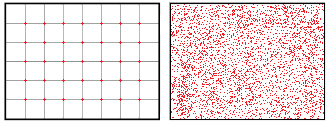
\includegraphics[width=\linewidth]{img/GridVsRand.png}
  \caption{ (a)Grid with uniforme and regular distribution.\\   
(b) Random distribution.\\  
}\label{fig:GridVsRand}
  \endminipage\hfill
  \end{center}
\end{figure}
%%%%% FIGURE  random distribution  form 171*
\begin{figure}[t!]
\begin{center}
\minipage{0.65\textwidth}
   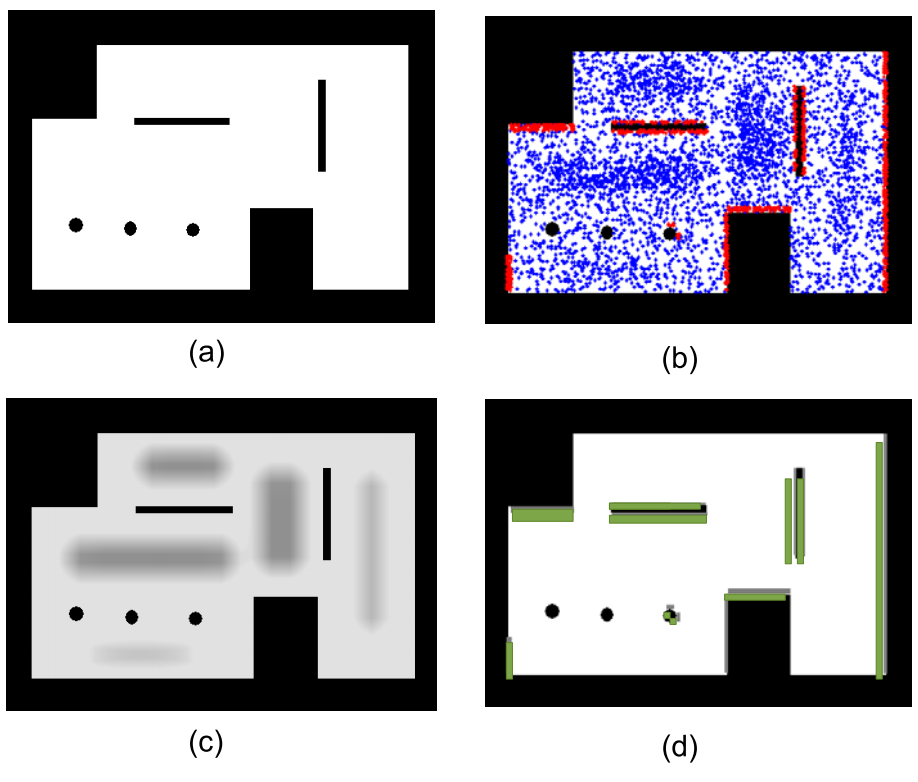
\includegraphics[width=\linewidth]{img/randomGridRef171.png}
  \caption{ (a )area  to cover.\\   
(c) Importance of the area.\\  
(b) grid representation.}\label{fig:randomGridRef171}
  \endminipage\hfill
  \end{center}
\end{figure}

 In the  \cite{83*van2009,171*horster2006} the random distribution is used to describe the area to cover. \\
In Hoster et al \citep{171*horster2006} the point of the grid are randomly distributed to describe all the area to cover. The advantage of this article is to use the random distribution in order to manage the density of points in some specific region of the area. Especially, by increasing the density of points on some specific zones of the area. The increased density allocates more importance to these zones (see Figure \ref{fig:randomGridRef171}).\\
Indeed the higher density will affect the optimization process. The area with more density will be comparatively more profitable to a low density area. In these cases, the zones with high density are covered in priority. This mechanism is even simplified due to the random distribution.

The hengel et al \cite{83*van2009} have tested the random distribution and the uniform grid pattern distribution before to conclude the grid pattern and the random distribution proposes globally the same result, when there is no priority zone in the area. Based on this observation hengel et al \cite{83*van2009} decide to use the uniform grid notably because of its simplicity of implementation.

%///////random distribution   for reduce the uniforme grid //////////
The "random distribution" is less popular but in \cite{22*zhao2008} a hybrid distribution is proposed. The idea proposed is to reduce the number of points in the uniform grid when it has a to hight density. To reduce the number of points in a random  selection is used. 



\paragraph*{ Special modelling (3D  or 2D)}
To design the occupation grid, one other element should be taken in consideration. It is the spacial modelling. After deciding the useful density and the distribution of the grid, the position in the space of the point $g_i$ need to be studied.  
In fact depending on the problem the grid can be modelled differently in order to properly cover the area to control. Commonly the occupation grid is placed on the floor and calculate visibility only in 2D  by computing the  camera projection as in  \citep{164*valente2013,150*chakrabarty2002,8*zhou2011,170*yabuta2008,171*horster2006,22*zhao2008}, but depending on the context the grid have interest do describe a 3D space.  
Hegle et al\cite{83*van2009}, calculates the visibility, where it is relevant: for example, on the upper torso or head of the possible target rather than the floor. This article  proposes a 2D grid but inside the 3D space in order to  characterize properly the volume by placing the grid at a specific height.  

In \cite{82*chrysostomou2012} the grid is formalized in the full volumetric space by numerous “control points” (as $g_i$) to control the area. The points of the grid is uniformly (or can be randomly) distributed along the axis of $x, y$ and $z$. Also in \cite{87*morsly2012} the grid are formulated in the volumetric space by using a uniform 3D grid distribution. The formulation proposed show the complexity even more important to use a 3 dimensional occupation grid and for practical reasons (mostly the inadequacy has computational power due to the increased complexity) the 3D grid is replaced by a 2D grid at a specific height to optimize the coverage. \\ 

While an occupation grid designed to estimate the volume cover along the $ x, y $ and $ z $ axes of the area already exist. His implementation is unusual due to the increasing complexity of the optimization process.  
Nevertheless some solution was discussed \citep{141*akbarzadeh2013,83*van2009} to take into account the volume of the area to cover which cannot be only limited to an occupation grid along the axes $ x $ and $ y $as a simple 2D grid.

In \cite{83*van2009} is focussed on estimating the area to cover inside a 3 levels of a building. To estimate the coverage in the building the grid was placed at each level. This solution is efficient in order to limit the number of points compares then a full volumetric description of the area. Also this design allows to keep the 3 dimensional information by adding a layer at each level of the building.  

In \citep{141*akbarzadeh2013} propose a 2D grid adapted to the relief of the area. This article are focused on covering a large outside area with an important relief. To estimate properly the area to cover a grid has been placed following the altitude of the relief as showed in Figure\ref{fig:grilleRef141}. 

%%% figurir  from 141*
\begin{figure}[t!]
\begin{center}
\minipage{0.65\textwidth}
   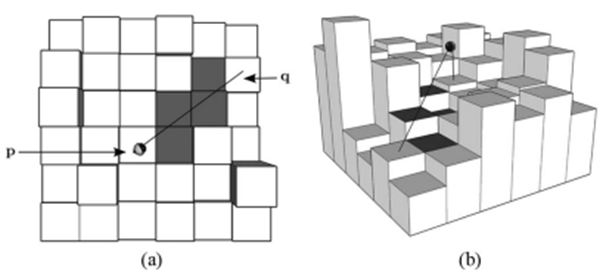
\includegraphics[width=\linewidth]{img/grilleRef141.png}
  \caption{ Relief grid use to discretize  an area with taking in account the relief.}\label{fig:grilleRef141}
  \endminipage\hfill
  \end{center}
\end{figure}

\paragraph*{Zones of interest.} 
Among the area to cover some zones may have a particular interest to be covered. These zones can be discriminate, by the grid design. 
The zones of interest are designate by different manner depending than the goal. Manly 3 methods can be discerned.
\begin{itemize}
	\item[-]	The multi coverage zone. 
	\item[-]	The priority zone.  
	\item[-]	Non-interesting zone.
\end{itemize}
 

\subparagraph{The multi coverage zone.}
The aim  of the multi coverage zone is to have on a specific zone of the area controlled by numerous cameras.  Multiple coverage may be called $k$-coverage as in \cite{174*zhang2016}. Where refers $k$ to the number of cameras mandatory to cover the zones of interest. 
Every points of the grid $G$ should be covered at least by one camera and for some specific zone of the area by $k$ cameras.\\
 Consequently a binary list of points is created to count the covered part of $G$ which are noted as $Pc$.

\begin{equation}\label{eq:PciK}
Pc_i= \begin{cases} 1, & \mbox{if } g_i\mbox{ is covered by $k_i$ cameras} \\ 0, & \mbox{otherwise}   \end{cases}k_i \in K
\end{equation}
Where $k_i$ is the number of cameras uses to cover the point $g_i$ of the grid. $K$ is the list of $k_i$ associate to the number of points in the grid. The list $K$ is initialized at one by default, except for the zones of interest where have to be superior to one as in \cite{82*chrysostomou2012}. 

\subparagraph{The priority zones.}
The zones to cover in priority are used especially in the case where the number of cameras are not sufficient to fully cover the area. This priority of coverage can be expressed by different way. \\
In the case where the grid is uniformly distributed a weighting may be fixed on the zone of the area to cover in priority \cite{141*akbarzadeh2013,84*xu2011}. This method was implemented in \citep{141*akbarzadeh2013} to optimize the position of the camera on the road passing through the area to cover. \\
In \citep{171*horster2006} the weighting of the priority zone is made by increasing the sampling frequency of the zones thanks to random distribution  as in Figure \ref{fig:randomGridRef171}(b). Using this method the zones of interest are more dense and that push the optimization process to cover this area in priority (more density mean more interest).\\
Otherwise the priority zone in the uniform grid distribution can be formulate as: 
  \begin{equation}\label{eq:PciP}
Pc_i= \begin{cases} 1*p_i, & \mbox{if } g_i\mbox{ is covered and  $p_i$ is the weight} \\ 0, & \mbox{otherwise}  \end{cases}
\end{equation}
Where $p_i$ is the weight of the point $g_i$ on the grid $G$. $P $ is the list of $p_i$ which contain the weighting of the area associate to the points of the grid $g_i$. \\

\subparagraph{Non-interesting zone.}
Non-interesting zones are the zones without interest to be covered noted $U$, with the set $U$ composed of points $g_i$. These zones are not strongly prohibited. That mean the zones considering as non-interesting can be covered but their coverage or un-coverage has no impact on the estimation of the coverage of the area. In the case of random grid, distribution the non-interesting zones have a sampling frequency null as in \citep{141*akbarzadeh2013}. For uniform grid distribution in the non-interesting zones are removed to the list $Pc$. This method is currently used like in \cite{22*zhao2008,170*yabuta2008,141*akbarzadeh2013,171*horster2006,84*xu2011} . 
\begin{equation}\label{eq:setU}
Pc=G-U \mbox{ ,    }  \mbox{ }U= \{ g_i | g_i \in G, g_i \mbox{ are the non intresting points} \}
\end{equation}


Finally  these methods use to design the zones of interest are not fully independent and can be associate with the same model as in \cite{141*akbarzadeh2013,171*horster2006,84*xu2011}. The combination of all these  zones of interest can be formulated as : 
 \begin{align}\label{eq:PcFull}
Pc_i= \begin{cases} 1*p_i, & \mbox{if } g_i\mbox{ is covered  by $k_i$ and  $p_i$ is the weight} \\ 0, & \mbox{otherwise}  \end{cases}
\\ Pc=G-U \mbox{ ,    }  \mbox{ }U= \{ g_i | g_i \in G, g_i \mbox{ are the non intresting points} \}
\end{align}

   
\paragraph*{Atypical design}  

Previously the method to set-up a classical occupation grid depending on the problem has been discussed. Few other solutions more atypical have been developed. On solution coming from the field of wireless sensor network is the topologies grid. 
 The topologies grid is clearly explained in Chakraborty et al \cite{150*chakrabarty2002} the interest of these methodologies is to reduce the number of points to cover. But in this case the number of points is not related to the resolution wished  but by the sensor range. Indeed the size between the point of the grid has been defined by the size of the minimum range of the sensors. The distance of the minimum sensor range are used as nodes for a topological relation. \\
Another atypical solution is to develop a grid composed by rectangles. Each rectangle may have different size adapted to the obstacle in the area. A rectangle is considered as covered if most of the area of the rectangle is covered by the cameras as in \citep{170*yabuta2008}. This method is adapted to the area with few obstacles as is shown in the Figure \ref{fig:from170}.
\begin{figure}[t!]
\begin{center}
\minipage{0.65\textwidth}
   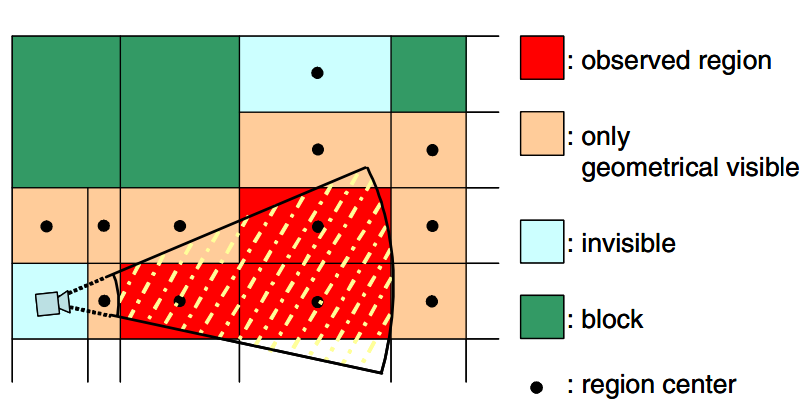
\includegraphics[width=\linewidth]{img/from170.png}
  \caption{ Observed regions from camera candidate.}\label{fig:from170}
  \endminipage\hfill
  \end{center}
\end{figure}

\newcolumntype{M}[6]{>{\raggedright}m{#1}}
\paragraph*{Grid sum up}
 tableau for summarize  the grid modeling
 \begin{center}
   \begin{tabular}{ l | m{0.1\linewidth} | m{0.1\linewidth} | m{0.187\linewidth} | m{0.187\linewidth} | m{0.187\linewidth} |  }
     \hline
     ref & grid pattern & grid random  & volumetric space & Sampling frequency &Zone of interest \tabularnewline \hline 
	 \cite{8*zhou2011}   		&	 X	 &	     & 	   						  & For real-time    & X \tabularnewline   \hline 	
	 \cite{22*zhao2008}  		&	 X	 &	 X   & 	   						  & Incremental	 	 & X \tabularnewline \hline     
	 \cite{82*chrysostomou2012} &	 X	 &	     &	3D grid					  &  				 & X \tabularnewline \hline
       \citep{83*van2009} 		&	 X	 &	 X   & 	2D grid at each level  	  &  				 &	\tabularnewline \hline
    \cite{87*morsly2012} 	 	&	 X	 &	     &  Superposition of 2D grid  &  	Adaptable	 &	\tabularnewline \hline
\cite{141*akbarzadeh2013}       &	 X	 &	     & 	2D grid on relief 		  &  		 		 & X \tabularnewline \hline
   \cite{150*chakrabarty2002}   &	 X	 &	     & 	  	 					  & Topologies sensor&	\tabularnewline \hline
     \cite{164*valente2013} 
     &	 X	 	&	     &overlap by shifting of z  &  				 &	\tabularnewline \hline
      \cite{170*yabuta2008}     &	 .	 & 	     &		  					  &For zone 
     															segmentation 	 & X \tabularnewline \hline
      \cite{171*horster2006}    &	  	 &	 X   & 	  	 					  &  		 	 	 & X \tabularnewline \hline
      \cite{174*zhang2016}      &	  	 	&	     & 	 	 					  & 				 & X \tabularnewline \hline
           
   \end{tabular}
 \end{center}
	 
\subsubsection*{Our approach}
 Base on the different design the one finally adopted is a grid $G$ as in Eq \ref{eq:Grid} with an uniform repartition following the 2D grid pattern. The frequency adopted is fixed depending than the size of the area, the precision required and the cameras property. The frequency adopted for the following part as to be considered as dense (high sampling frequency).
  The grid is placed on the floor of the area to control. Floor is always considered as flat without relief. The zone of interest can vary depending on the need of the experimentation, but the design chosen is flexible to apply if necessary the formulation form the Eq:\ref{eq:PcFull} with mostly $k=1$ and $p=1$, also a set $U$ is used to represent the non-interesting zone as it was presented in eq \ref{eq:setU}.

%%%%%%%%%%%%%%%%%%%%%%%%%%%%%%%%%%%%%%%%%%%%%%%%%%%%%%%%%%%%%%%%%%%%%%%%%%%%%%%%%%%%%%%%%%%%%%%%%%%%%%%%
%%%%%%%%%%%%%%%%%%%%%%%%%%%%%%%%%%%%%%%%%%%%%%%%%%%%%%%%%%%%%%%%%%%%%%%%%%%%%%%%%%%%%%%%%%%%%%%%%%%%%%%%
%%%%%%%%%%%%%%%%%%%%%%%%%%%%%%%%%%%%%%%%%%%%%%%%%%%%%%%%%%%%%%%%%%%%%%%%%%%%%%%%%%%%%%%%%%%%%%%%%%%%%%%%
\section{ Cameras coverage.}\label{sec:CamerasCoverage}


Once the area to cover is described by the grid, the next step is to verify for each point of the grid if one or more cameras cover it, based on Eq: \ref{eq:PciK} with $k=1$.\\
To verify if each points of the grid is covered by a camera. It is primordial to talk about what is a camera, what kind of camera are appropriate and their projection model. 

%%%%%%%%%%%%%%%%%%%%%%%%%%%%%%%%%%%%%%%%%%%%%%%%%%%%
\subsection{ Cameras definition.}\label{sec:CamerasDefinition}

The closest projection model to the human view is the perspective projection. The perspective projection is also the more common and more especially in the field of area coverage as in example \cite{101*topcuoglu2009,33*reddy2012,8*zhou2011,82*chrysostomou2012,22*zhao2008}. Other model of cameras or vision sensor can be used as for example omnidirectional with a $360^{\circ}$ of field of view as \citep{43*erdem2006,150*chakrabarty2002,174*zhang2016}. 
Here we are only focussing  on the camera perspective due to its wide use.  \\

The pin hole or in Latin the "camera obscura" is at the origin of the geometry model for the perspective projection.\\
\begin{figure}[t!]
\begin{center}
 \minipage{0.65\textwidth}
   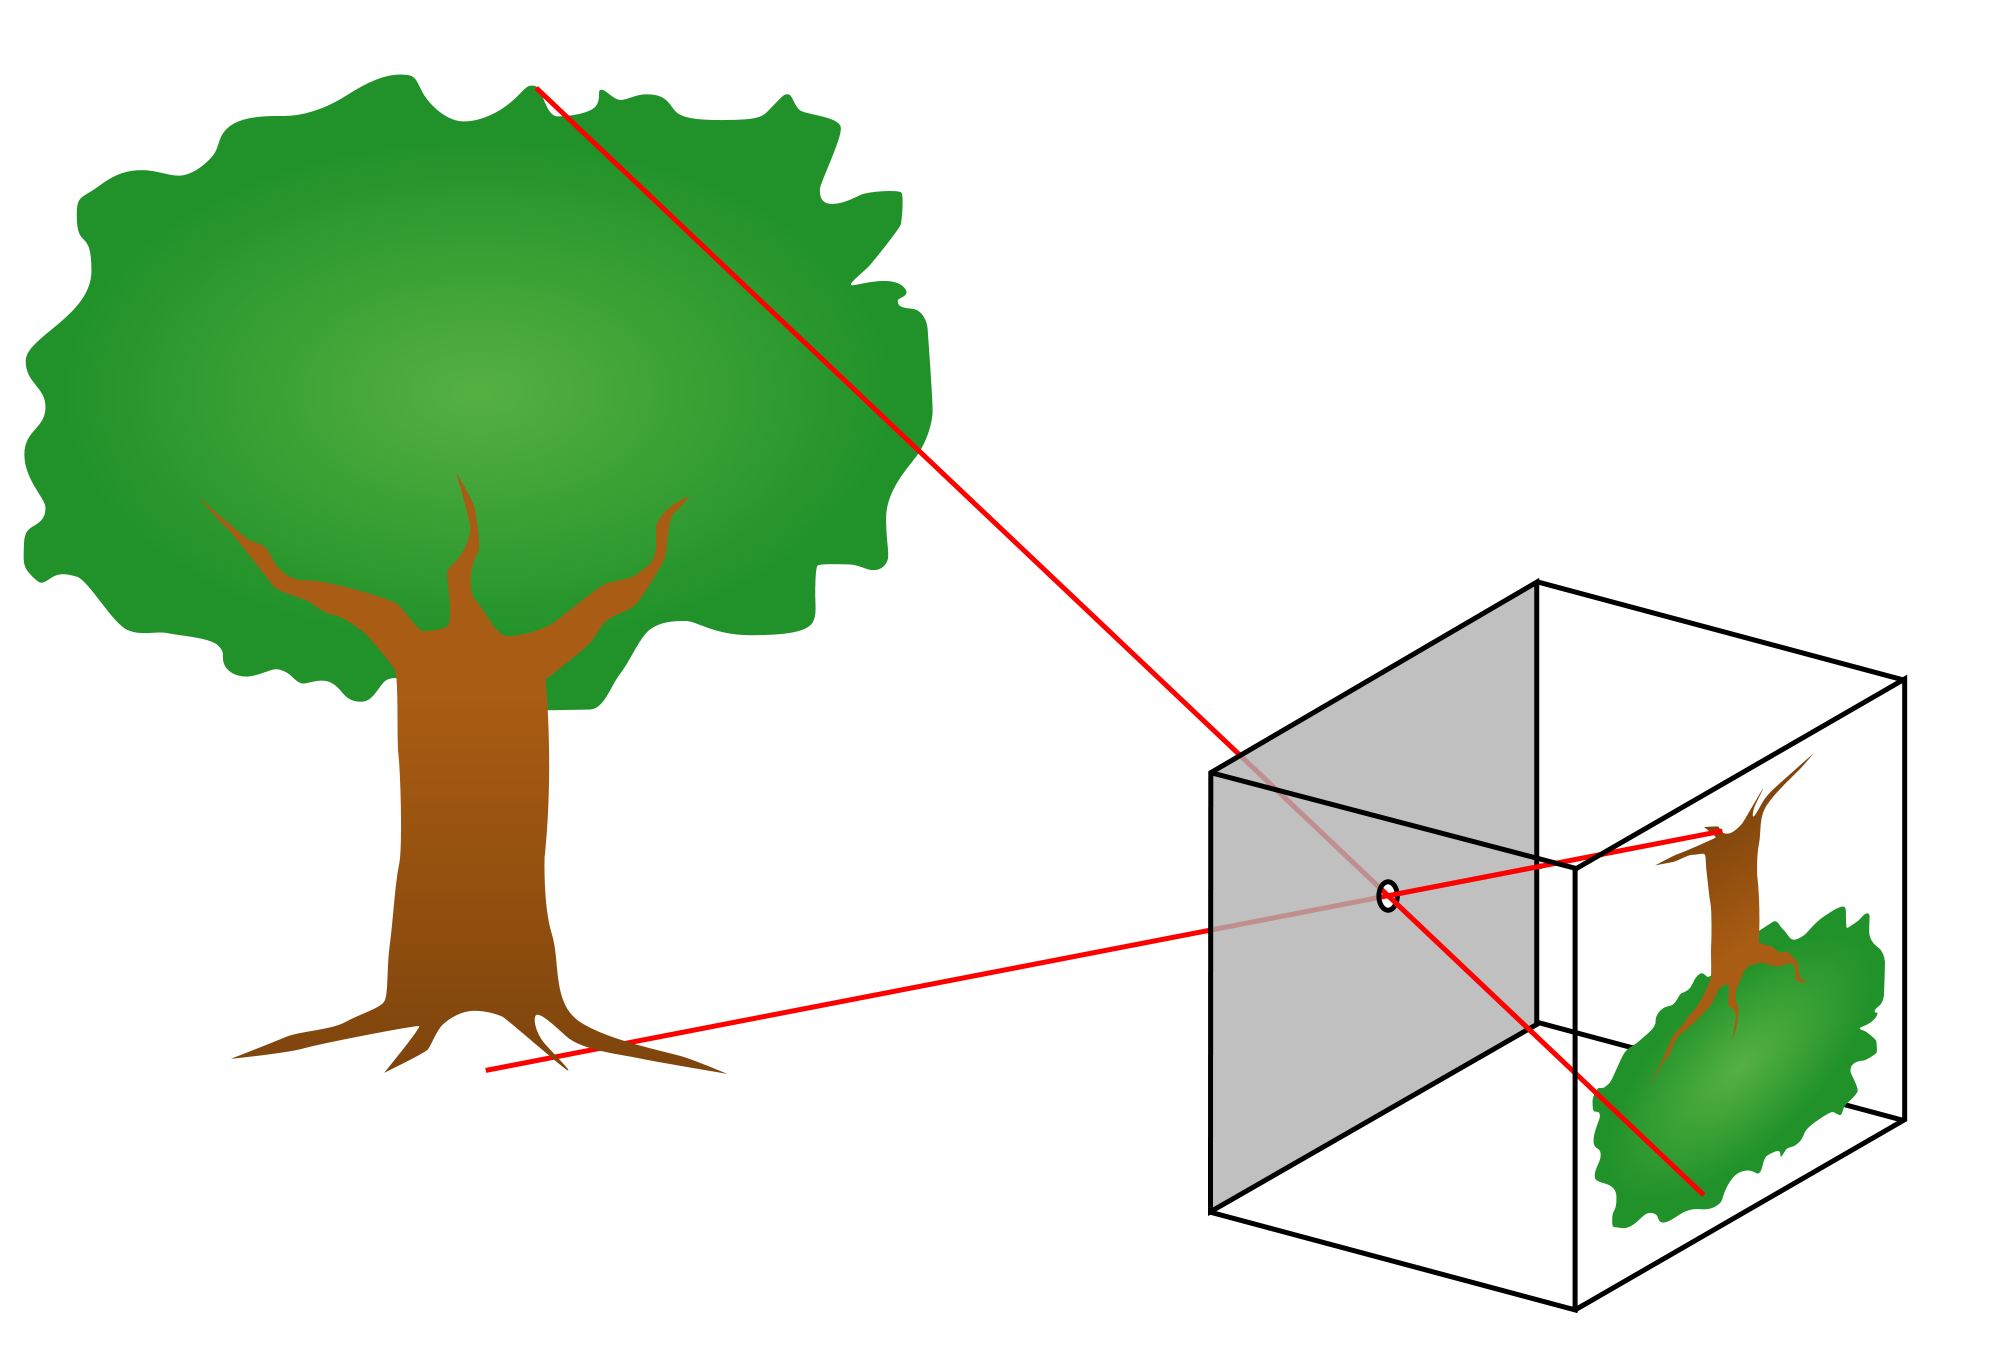
\includegraphics[width=\linewidth]{img/PinholeCam.png}
  \caption{ Pin hole camera model.}\label{fig:PanTiltRoll}
  \endminipage\hfill
\end{center}
\end{figure} 
 The pin hole model is commonly composed by box (or chamber) hermetically closed to light, excepted by a small pin hole on the middle of the front side. All the ray of light reflected by the object of the world and passing by the small hole are projected onto the back side of the box. Each ray of light passing by the hole is  projected on the plan (inside the box). This plan became the reversed image of the world and can be recorded by a film or a digital sensor. 
 Due to the simplicity of the pin hole model, the calibration and camera projection estimation is simplified.\\
  Based on it, the camera projection is dependent then few parameters intrinsic (as focal length, sensor size,...) and extrinsic (as the position $x,y,z$ and orientation $\alpha,\beta,\gamma$). 
  
 
\begin{figure}[t!]
\begin{center}
\minipage{0.65\textwidth}
   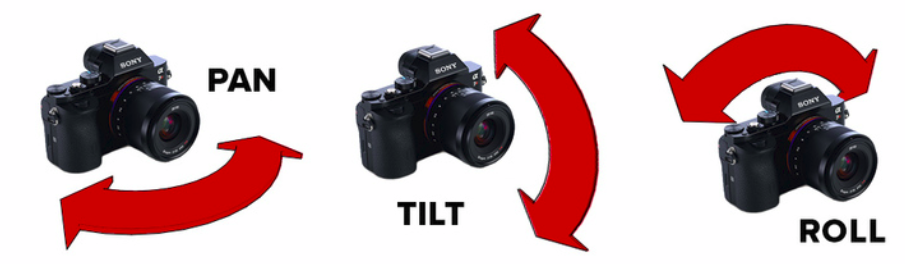
\includegraphics[width=\linewidth]{img/PanTiltRoll.png}
  \caption{The rotation composed by 3 degrees of freedom on pan tilt roll$(\alpha,\beta,\gamma)$.}\label{fig:PanTiltRoll}
  \endminipage\hfill
  \end{center}
\end{figure}

In fact the useful elements to define the projection of a camera perspective, can be stated as a set of parameters composed by:\\
\begin{itemize}
\item Three degrees of freedom of the sensor’s position: $(x, y, z)$;
\item Three degrees of freedom of the sensor’s orientation: with the  the rotation in pan, tilt, and swing angles: $(\alpha,\beta, \gamma)$ 
\item Optical parameters including: the focal length $f$ of the lens, the sensor size $s$, $u_{0}$ and $v_0 $  which would be ideally in the centre of the image. $\sigma_{uv}$ represents the skew coefficient between the $x$ and the $y$ axis.
\end{itemize}
$s$ is composed by two elements $Sw$ and $Sh$ for the size of width and height (also called  the scale factor).\\

Among the parameters of the camera, only  some of them are useful to estimate the projection. They can be formalized as a vector:
\begin{equation}\label{eq:v}
v=(x,y,z,\alpha ,\beta,\gamma,f,s,u_0,v_0,\sigma_{uv})
\end{equation}

Each element of the vector $v$ are used to compute the camera projection on the discretized floor. 
\iffalse 
To model the set of the cameras using the precedent notation, a set $V$ composed by $N$ cameras defined by $v$ noted:
\begin{equation}\label{eq:V}
\begin{split}
V= \{v_i\} \mbox{  , } \forall i=[1;N] \mbox{ , } N\in \mathbb{N}^*
\\
\mbox{ and } v_i= (x_i,y_i,z_i,\alpha_i ,\beta_i,\gamma_i,f_i,s_i,{u_0}_i,{v_0}_i,{\sigma_{uv}}_i)
\end{split}
\end{equation}
\noindent Where $N$ is the given number of cameras in the solution. Which is also the number of cameras in the set $V$. \\
Therefore, $V$ represent a camera networks and also a initial set of parameter for a set of cameras. $V$ can contain all the possibility, included the non-acceptable answer. A non acceptable  answer will be an answer with  doe's not respect the constraint of the problem.   
 \\ !!!!!!\\

%%%%%%%%%%%%%%%%%%%%%%%%%%%%%%%%%%%%%%%%%%%%%%%%%%%%  
  
 
    
The hole in the box is called the projection center. It is the point were each ray of light are crossing together.  \\
Based on this model, a 3D point $^CP=(^Cx,^Cy,^Cz,1)^T$ defined in the pin hole reference noted $ ^C\Re$ can be convert in to a 2D point  $^rp=(^ru,^rv,1)^T$ in the sensor reference (back side of the box) by using  the perspective projection model $pr() $: 
\begin{equation}
^rp=(^ru,^rv)= pr(^CP) \mbox{ with } \begin{cases} u= f.\frac{^Cx}{^Cz} \\  v= f.\frac{^Cy}{^Cz} 
\end{cases} 
\end{equation}
Where $f$ is the focal length (distance between the projection center and the photosensitive sensor )
the point $^rp$ is the projected point $^CP$ on the sensor. The sensor is composed by $sw$ pixel of width and $sh$  pixel of  heigh. To convert the coordinate $^rp$ of p in the pixel  that mean in the image reference $^i\Re$ : 
\begin{equation}
^ip=K. ^rp
\end{equation}
where $^ip$  is the point $p$ in the image reference composed by $(u,v) \in ^i\Re$ with $u$ and $v$ are  pixel coordinate. 


%Where $u_0$ and $v_0$ are the coordinate  of  the principal point of the image ( projection of the optic centre on to the image plan).  
%$k_u$ and $k_v$  are the magnification factors of the image on width and heigh. 

% resource http://ksimek.github.io/2013/08/13/intrinsic/
%https://jeux.developpez.com/tutoriels/OpenGL-ogldev/tutoriel-12-projection-perspective/
The cameras is called calibrated when the intrinsic parameters ($K$)are defined.  
 The intrinsic matrix $K$ is parametrized by Hartley and Zisserman and it is composed permit to represent the properties of the camera. To design the intrinsic matrix $K$ some part of the pin hole camera have to be defined :\\
  \begin{itemize}
  
 	\item $f$ is  the focal length. The focal length is the distance between the pinhole and the sensor (a.k.a. image plane)
  	\item $k_u et k_v$ are the magnification factors of the image on width and heigh ; related to the image sensor format%  les facteurs  aggrandisement de l'image 
  	\item $u_0 v_0$  are the coordinate  of  the principal point of the image ( projection of the centre optic on to the image plan)  %the les coordonnées de la projection du centre optique de la caméra sur le plan image 
  	%\item $s_uv$ qui traduit la non-orthogonalité potentielle des lignes et des colonnes de cellules électroniques photosensibles qui composent le capteur de la caméra. La plupart du temps, ce paramètre est négligé et prend donc une valeur nulle.\\
  	  \end{itemize}
		Once these elements are known the matrix $K$ can be designed :
	\begin{equation}
		K=
		\begin{pmatrix}
			k_u 	& 0 	& u_0 \\
			0 		& k_v	& u_1\\
			0 		&	0	& 1
		\end{pmatrix} .
		\begin{pmatrix}
			f 		& 0 	& 0  \\
			0 		& f		& 0  \\
			0 		&	0	& 1  
		\end{pmatrix} 
	\label{eq:K}
	\end{equation}
Finally, in order to estimate the positions of a 3D point in the pin hole camera reference $^C\Re$ in to the image reference $^i\Re$ 
$$
^ip=K.pr(^CP)
$$ 	  
 Parameter extrinsic (definition global) \\
  \begin{itemize}
 	\item$R_3x3$ = la matrice de rotation permettant de passer du repère lié à l'espace de travail au repère lié à la caméra\\
 	\item$t_x t_y t_z$ = les composantes du vecteur de translation permettant de passer du repère lié à l'espace de travail au repère lié à la caméra.\\
  \end{itemize}
 %Parameter utile pour notre cas de figure \\     fig : \ref{eq:V}\\
 
!!!!! the previous section can be largely (keep the basic introduction remove to be replace by ... !!!!!
\fi
%%%%%%%%%%%%%%%%%%%%%%%%%%%%%%%%%%%%%%%%%%%%%%%%%%%%%%%%%%%%%%%%%%%%%%%%%%%%%
\subsubsection{Coverage estimation in the literature}

%To estimate the coverage of a set of camera $V$  the cameras projection of each $v_i$ has to be computed individually.
 In order to compute the camera projection onto a grid the pin hole model is used with the parameters of the vector $v$.\\
The detail to estimate the camera projection on to the floor, based on the pin hole model and the parameters ($v$), has been detailed numerous times as in \cite{193*fu2014,181*wang2017,165*jiang2010}. In \cite{193*fu2014,181*wang2017,165*jiang2010} the camera projection is used to estimate if a point is visible by a camera, for each point of the grid. These articles handles the classic camera projection (with the 6DoF in \citep{193*fu2014} and 5DoF in \citep{181*wang2017}), both are used to estimate the 2D projection of the camera onto the floor. \\
In  \citep{193*fu2014}, the camera projection has been computed for several rotations for all the DoF. In this case, the projection can have numerous shapes (mostly parallelogram shape).
In \citep{181*wang2017}, the model of camera projection begins to be simplified by assuming some fixed parameters. The fix parameters allow more efficient by economizing part of projection computation of the camera at each time.  \\
In \citep{165*jiang2010}, the model of camera projection is used to compute one time for a fix pan and roll in order to have a coverage estimation use in a 2D map. The camera projection is finally simplified by using a kind of triangle shape.\\
 Some of them as \citep{165*jiang2010,181*wang2017,141*akbarzadeh2013} include the object occlusion. To detected the part of the area occluded by an object, the solution commonly proposed (as is well explain in  \citep{181*wang2017}) is to check the line made between a point covered ($g_i \in Pc$) and his camera. If this line is intersected by at least one object in the scene, the point $g_i$ cannot be considered any-more as covered. 
%  Despite the simplicity of the computation numerous operation have to be done to compute the camera projection onto the floor. \\

To go further other model and formulation inspired by the pin hole model has been proposed as \cite{87*morsly2012,141*akbarzadeh2013,146*li2011,194*fu2010}. These models are inherited for the camera projection and adapted to fit their problems. \\
In \cite{87*morsly2012,194*fu2010} the camera is considered to be placed on the floor with a fix pan (with the looking direction almost parallel to the floor). Therefore the camera projection is simplified by an isosceles triangle where the shape depends on the focal length.\\
In \citep{141*akbarzadeh2013} the camera projection is also simplified in order to have a kind of isosceles triangle shape with considering the depth of view of the camera.\\
In \citep{146*li2011} thanks to a fix pan and focal length, the camera projection is simplified in order to have a rectangle projection onto the ground. The sweep is designed consequently to the size of the camera projection, in order to minimize the overlap and have full coverage of the area.  


One of the common point of the method present in \cite{87*morsly2012,141*akbarzadeh2013,146*li2011,194*fu2010,22*zhao2008,33*reddy2012,193*fu2014,181*wang2017,165*jiang2010}   is the computation of a camera projection on to a grid. The computations necessary to estimate, if a point of the area is cover are not considered as really greedy (in time). But have to be done to each point $g_j$ of the grid and for each camera $v_i$ of the network.
	\begin{equation} \label{eq:sum sum v g}
		\sum_{j=1}^{m}\sum_{i=1}^{n}f( v_i,g_j)
	\end{equation}
Where $n$ the number of cameras in the network; $m$ the number of point in the grid; \\
This equation (Equation \ref{eq:sum sum v g}) does not take in account the occlusion by few obstacle $Obj$. If we add the potential occlusion by $k$ object: 
	\begin{equation}
		 \sum_{k=1}^{k}\sum_{j=1}^{m}\sum_{i=1}^{n}f( v_i,g_j,Obj_k)
	\end{equation} 
 
The function $f(...)$ in charge to compute a camera projection will be called in the worst case for each camera, in order to evaluate the complete coverage of the area. This numerous call will greatly increase the time computation of the coverage. It is even worst when numerous cameras projection ($n$) has to be computed at each turn of a long optimisation process.\\
In this condition the efficiency of the function $f()$ in charge then, computes the coverage estimation is primordial, due to the numerous call.



\subsubsection{Coverage estimation optimization} \label{sec:coverageEstimation}
Design an efficient cost function is necessary to reduce the time computation and estimates the area covered. A good estimation of the area covered is primordial for the optimisation process. 
  The computation of a camera projection have to be minimized with some basic assumption depending on the problems.\\
Considering our case, where a camera is fixed on a UAV with a looking direction orthogonal to the ground, without any rotations in $\alpha$ (pan) and $\beta$ (tilt). It is possible to compute for a given altitude the area covered by one camera, based on the given parameters. Especially the focal length $f$, the altitude of the cameras and the sensor size $s$. Where $s$ is composed of $Sw$ sensor size width and $Sh$, sensor size height ($s= [Sw ; Sh]$). 
In this model the camera projection is always a rectangle as described in Figure \ref{fig:cam_proj}. To estimate the shape of the rectangle with is deduced from the ratio of $s$ and the size of this rectangle with is deduced from $(f ,s ,A)$. Where $A$ is the altitude. The altitude is the distance between the grid and the cameras, in the simple case $A$ is considered to be equal to $z$, when the grid is on the floor.  \\
The basic computation to estimate the size of a camera projection :

%\begin{equation}
%s= [Sw ; Sh]  %\mbox{   } Sw,Sh \in \mathbb{N} 
%\end{equation}
%
%\noindent Where $Sw$, sensor size width. \\
%Where $Sh$, sensor size height.
	\begin{equation} \label{eq:etaUpsilon}
 	 \begin{split}
		\eta = 2\times \tan^{-1} (\frac{Sw}{(2\times f)}  ) 
 	   \\
		\upsilon = (\frac{Sw}{Sh} )\times \eta
 	 \end{split}
	\end{equation}
Where $\eta$, $\upsilon$ are the horizontal and vertical camera fields of view.\\
Estimating the width and height of the rectangle projected on the ground depend on the altitude $A$ :
	\begin{equation}\label{eq:WrHr1}
		\begin{split}
    		Wr= 2\times A\times\tan \eta
    	    \\
    	    Hr= 2\times A\times\tan \upsilon
    	 \end{split}
	\end{equation} 
	\begin{figure*}[t!]
		\centering
		\minipage{0.85\textwidth}
  		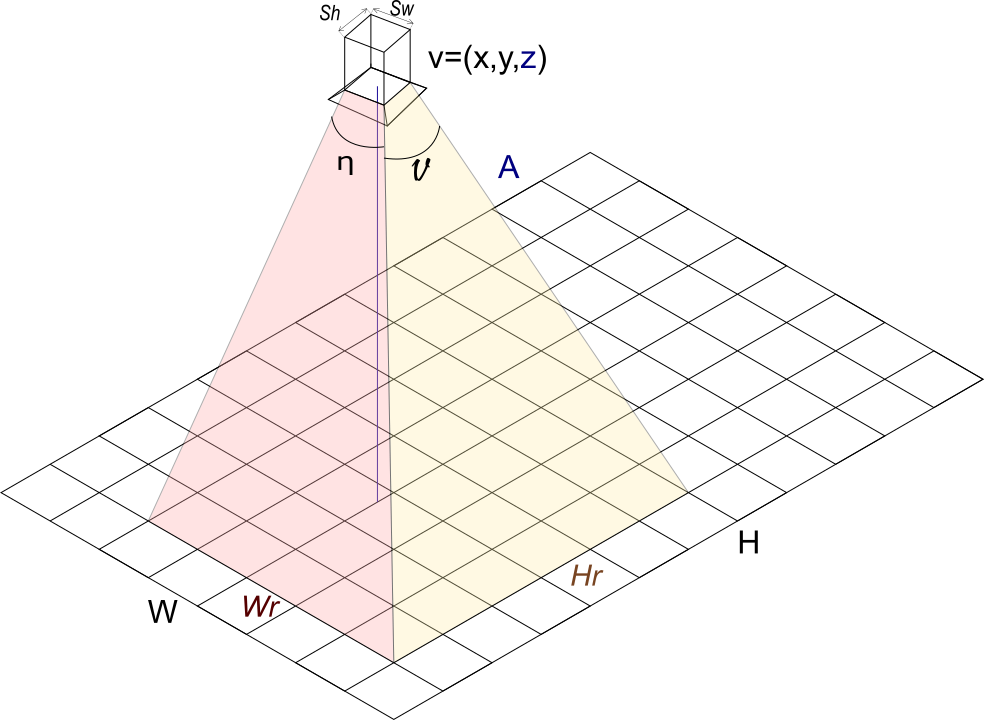
\includegraphics[width=\linewidth]{img/CamProject1Bis.png}
  
 	 	\endminipage\hfill\caption{Camera projection onto a grid. The grid is placed on the floor to discretize 	the area covered.}\label{fig:cam_proj}
	\end{figure*}

Therefore, the size of the rectangle projected onto the floor is $(Wr,Hr)$ for the width and height. The values of $Wr$ and $Hr$ are directly linked to the altitude of the camera. In the simple case and in the initialization, $A$ is equal to $z$  and $z$ is selected in a range given by the UAV or the user. \\
Once the couple $(Wr,Hr)$ as been computed for a $A=z$ it is easier to change the altitude of the camera. The rectangle projection will be affected in proportion.
	\begin{equation}\label{eq:A.coef}
		\begin{split}
 		   	f(A)= (Wr,Hr) \text{ based on eq \ref{eq:WrHr1}}\\
    		f(A.Coef)=f(z)= (Wr.Coef,Hr.Coef)      
    	 \end{split} 
	\end{equation}
Therefore, to any altitude $z$ is existing $A.Coef$ where the size of the camera projection onto the floor is $(Wr.coef, Hr.coef)$. Thanks to this the eq: \ref{eq:etaUpsilon} and eq: \ref{eq:WrHr1} have to be compute once  for a given focal length $f$ and sensor $s$ with an simple $A=z$. Adding simple $Coef$ the size of camera projection can be easily simplified in order to limit the useless computation (only 2 multiplication instead then equation \ref{fig:cam_proj} and \ref{eq:etaUpsilon}.
The model of camera projection is greatly simplified by the UAV assumption (fix pan, tilt and focal length). That permits to consider the camera projection as a simple rectangle with a size directly related to the altitude (by using a simple coefficient $Coef$).\\
%The simplification by modelling all the cameras with a fix orientation and same ability (in order to have a rectangle projection onto the ground) 
All this simplification helps the cost function to be fast and efficient. \\

\subsection{Parameter to optimize }\label{sec:parameterToOptimize}
% en raison de 
By dint of the simplification presented previously the vector of parameters (\ref{eq:v}) can be simplified too.\\
To summarize,  the computation of one camera projection onto the floor, where the floor is represented by a grid for the area to cover, and the camera is in altitude with a looking direction orthogonal to the floor. Just few parameter are necessary  as showed in equation  \ref{eq:etaUpsilon} %{eq:WrHr1 , }
to \ref{eq:A.coef}. Thanks to that the equation (\ref{eq:v}) can be reduced with keeping only the position of the camera and the roll as:
	\begin{equation}\label{eq:v2}
		v=(x,y,z,\gamma )
	\end{equation}
	or also
	\begin{equation}\label{eq:v2}
		v=(x,y,A.coef,\gamma )
	\end{equation}

Reducing the number of  parameters, passing to the equation \ref{eq:v} to \ref{eq:v2} are really usefully to the optimisation of the problem. The reduction of the number of parameter will greatly affect the optimisation process.\\
 Indeed, in addition to reduce the time computation, this simplification reduce the number of parameters to optimize.   

Until now the camera projection estimation as was addressed with only one camera. But we want to compute the coverage for a set of cameras. \\
The solution is based on the previous estimation for the camera projection, but adapts to the location of each camera. By  positioning the rectangle projection to have the center of it at the $x$ and $y$ position and compute the occupation grid.\\

In order to win a bit of time, each point of the grid already cover by a camera are note tested for the next cameras. This small modification will impact positively the computation time for the coverage estimation of a network of camera. That mean in the equation \ref{eq:sum sum v g} the value of $m$ decrease as $i$ increase. More exactly  the size of $m$ decrease as  the area coverage increase.  
\\

\subparagraph{Representation of the parameters to optimize. \\}

Until now, the camera formulation is adapted to one camera, to represent the problem we need a set of cameras. The precedent notation can be extended to have a set of $V$ composed by $n$ cameras defined by the parameters of $v$:

	\begin{equation}\label{eq:V}
		\begin{split}
			V= \{v_i\} \mbox{  , } \forall i=[1;n] \mbox{ , } n\in \mathbb{N}^*
				\\
			\mbox{ and } v_i= (x_i,y_i,z_i,\gamma_i)
		\end{split}
	\end{equation}
\noindent Where $n$ is the given number of cameras in the network. The coordinate of a camera $v_i$ with are the $i$th camera of the network is defined  with $x_i, y_i, z_i,$ for a given room and $\gamma_i$ the roll rotation (portrait or landscape). The parameters not contained in $V$ and used to compute the cameras projection are  identical for all the set $V$, and are fixed at the beginning of the optimization.\\
Therefore, $V$ represents a solution. $V$ contain all individual positions and orientations of the set of cameras for a predefined focal length, sensor size and map depending on the problem.% wish also include the potential constraint as  some restriction on the map.\\
Obviously all the solution $V$ are not a "possible solution" for our problem. Some solution $V$ does not respect the set of constraint noted $E$.

So that the $V$ should respect the constraints of the set $E$ (see Eq.\ref{eq:Vs}). Among the constraint few of them was already disused, as the occlusion, the map restriction, the k-coverage, or some constraint more specific to the problems (as saw in chapter \ref{chap:stateOfTheArt}).\\
 The "possible solution" $Vs$ must take in consideration with the set $E$ as :

\begin{equation}\label{eq:Vs}
Vs=V \mbox{ , iff } E(V)=\begin{cases}1, & \mbox{  iff } E_i(V)=1 \mbox{ , with } i=1...Nc \\ 0, & \mbox{otherwise} 
\end{cases} 
\end{equation}
Where $E_i(V)$ is the function applied to verify  the $i$th constrains of the set $E$ on the solution $V$. $Nc$ is the number of constraints needs to be satisfied to have an acceptable solution.
That mean among all the possibles combination of parameters $V$ only the one intersect the set of the constraint $E$ are an possible solution.  If we are considering  all the $V$ and all the $E$ as two subset $Vs$ is defined as $Vs=V\subset E$. 

The problem of monitoring an area and more specifically the problem of area coverage may contain many constraints depending of the environment and the context. As example: the room shape, minimizing  the altitude,  have the best resolution, orientation of the camera, the possible occlusion,... All this constraints are included in the set $E$. 
The constraint have to be defined depending on the problems and the goal.

\section{Constraint}\label{sec:constraint}

Make the exhaustive list of all the constraints for the problem of cameras positioning is not really interesting and almost impossible. The constraint can be numerous and depend mainly of the problem formulation and the context. Like that few of them was briefly introduced in the previous section as in chapter \ref{chap:stateOfTheArt}, section \ref{sec:coverageEstimation},... This part is focus on the list of the constraint used in our case and detail their design.

The constraint considered in this work are : 
\begin{itemize}
	\item Fix number of the cameras.
	\item Fix parameters of the camera.
	\item No rotation  on  $\alpha$ and $\beta$ (pan and tilt).
	\item Possible fix altitude.
	\item Altitude boundary (not too hight, not too low).  	
	\item The map boundary (rigid rectangle).  
	\item Non rectangles map with possible holes.
	\item To have some fix cameras in the set. 
	\item The resolution.\\

\end{itemize} 
\subparagraph{Fixes number of the cameras.}
One of the first constraint is the fix number of cameras. This constraint as some others (detailed latter) are  useful to simplify and restrict the possibility of the problem. This constraint permits us to focus on the fine optimisation (as in \citep{22*zhao2008} where both are tested). The number of cameras is fixed at the beginning of the optimisation and no more camera will be added during the optimization process.  

\subparagraph{Fixes parameters of camera and no rotations.}
Fixes parameters of the cameras and no rotations ($\alpha$ and $\beta$) has been introduced previously (section \ref{sec:parameterToOptimize}). These constraints imposed by the use of an UAV are also an advantage for the optimization by simplifying the coverage estimation and limit the number of parameters to optimize. The parameters are fixed at each beginning of the optimization.

\subparagraph{Fixes altitude.}
 The fix altitude is a constraint use in order to limit the number of parameters to optimize. The use of this constraint is used to reduce the complexity (see section \ref{sec:OptimizationComplexity}). It is also useful for other assumptions, as a camera on the celling or for a submarine  \cite{66*galceran2013}. This constraint is an optional constraint and is not commonly used in the experiment presented in the following section.   

\subparagraph{The altitude boundary.}\label{sec:altitudeBoundary}
 When the altitude is not fixed some limit must be chosen to avoid the extremely high and low altitude. The highest altitude will be fixed depending on the UAV ability and other restrictions as the laws. The lowest altitude has to be fixed for the safety of the user under the UAV.  
In practice the boundary of the $z$ is defined with :
 \begin{equation}\label{eq:boundaryZ}
   \inf z\leq A.Coef\leq \sup z  
 \end{equation} 
 Where $\sup z$ is the maximal altitude of the camera and $\inf z$ the minimum altitude. $A$ is the fix altitude  of a camera where the camera projection has been computed with $A=z$ with only $coef$ vary as introduced in Equation \ref{eq:A.coef}. 
 
 \subparagraph{The map boundary.}
The map boundary is a constraint similar then the altitude boundary. Despite the shape of an area to cover some maximum boundary can be made. In fact for any shape as complex as it, it is  possible to encapsulate in a rectangle. The rectangle map boundary is defined by a width $W$ and height $H$. The boundary on $x$ and $y$ are:
 \begin{equation}
  \begin{array}{lcl}
  	0\leq x\leq W \\
  	 0\leq y\leq H 
  \end{array} 
 \end{equation}  
 
By associating the altitude boundary (from Eq\ref{eq:boundaryZ}), a cube boundary limits the position of the cameras in the 3 dimensional spaces. 
\begin{equation}\label{eq:3dBoundary}
  \begin{array}{lclcl}
  	0\leq x\leq W \\ 0\leq y\leq H  \\ \inf z\leq A.Coef\leq \sup z  
  \end{array} 
 \end{equation} 
 
 \subparagraph{Non rectangle map with possible hole.}
Despite the rectangle boundary of the area, the map to cover can be much more complex than a simple rectangle and can take any kind of shape. Also the shape of the area can be composed by holes. The figure \ref{fig:boundaryMap} illustrate the map complexity. The black part of the map are the zone with are out. That mean these sub-parts have not interest to be covered.
 \begin{figure}[t!]
 \begin{center}
\minipage{0.85\textwidth}
   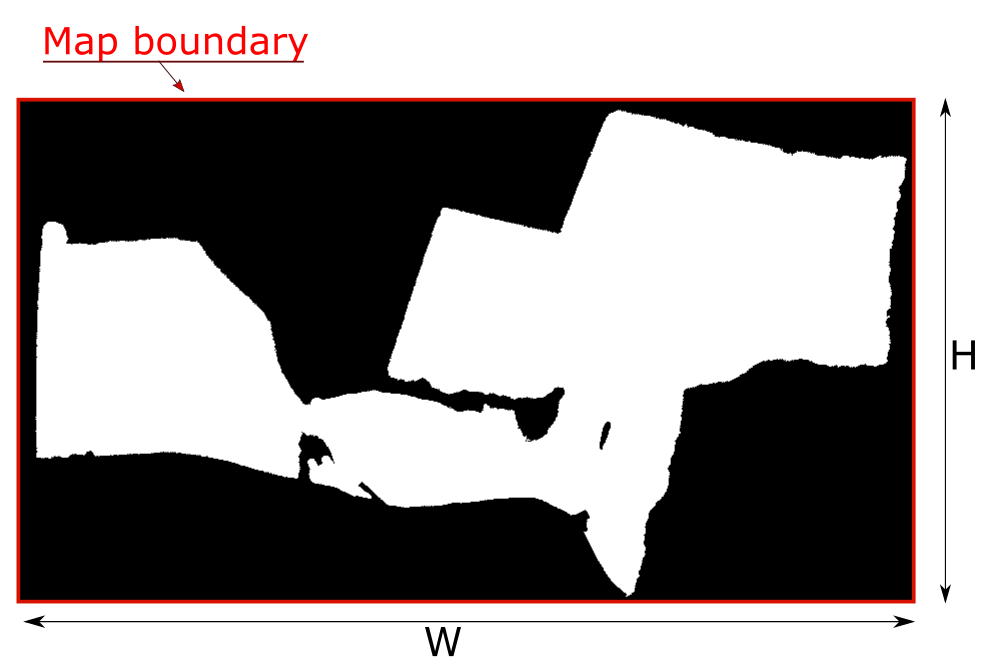
\includegraphics[width=\linewidth]{img/BoundaryMap2.png}
  \caption{Map to cover with the map boundary in red (W and H size) in black the sub-part have no interest to  be covered.   }\label{fig:boundaryMap}
  \endminipage\hfill
  \end{center}
\end{figure}
To take in account this constraint the gird has been designed with removing some of this points.
The grid $G$ is reduced in order to have only the points in the white sub-part. In this example each white pixel of the map is points of the grid. 
Concretely this implementation is easier for the complex map and has also some advantage. \\
Among the advantage, the flexibility of the grid customization. That allows the optimization to try some exotic solutions, as allowing the camera  position on the black sub-part or in a border of it during the optimization.  Obviously the exotic solution with a cameras position on the black side does not increase the coverage rate  but if the optimisation converge correctly no camera will be on the the black sub-part of the map (or small part of it).

\subparagraph{Some fix cameras in the set.}
Having some fix cameras position in the set of cameras, is an optional constraint. This allows to have few manual cameras position from an user or other algorithms.
One case can be to have some specific area as the entrance where have to be surveyed by a cameras dedicated to.  
To implement this constraint the solution applied during the experiments (presented later) is to adapt the map by removing the point of the grid $G$ cover by the sub-set of fix cameras (as if these points of the grid was covered).

\subparagraph{The resolution.}
The resolution of the images is related then the sensor size (in px) and the distance between the camera and the object filmed. In our case, the sensor size is fixed by the properties of the camera mounted on the UAV and the object filmed is the floor of the area to cover. In this case, the distance between the camera and floor is the altitude. \\
The resolution constraint has to maximize the resolution. In order to maximize the resolution during the optimization the altitude criteria is modified in order to be the lower possible.\\
Considering only the resolution constraint as minimizing the average altitude of the cameras is harmful for the coverage optimization.
Consequently, during the optimization a trade off between the altitude (and the related resolution) and the coverage rate have to be done $\min{\frac{\sum^n_{i=1}{A.coef_i}}{n}}$ and the coverage rate. In order to manage this trade off, the average altitude of the cameras is included in the cost function (see section  \ref{sec:costFun}).  
 
\subsection{Constraints types.}
 
Among the constraints listed different priorities and restrictions exist. Indeed the constraint can be considered in 2 sub-class. 

\subparagraph{Hard Constraint.}
 Some of the constraints presented are called "Hard constraint". \\
 The hard constraints limit the possible solution by do not allowing the solution with does not respect it. This hard constraint is directly used during in the optimisation process to prohibit any solution to be out of this boundary. This hard constraint has to be integrate in the optimization process in order to cannot generate a solution with does not respect it. Consequently the hard constraint can some times slow down the generation of the individuals.\\ 
 For example, the 3D boundary as defined in Equation \ref{eq:3dBoundary} is a hard constraint. Each cameras position must be inside the 3D boundary.\\
 
 \subparagraph{Soft Constraint.}
 In the other case, some constraint can be considered as "Soft Constraint".\\ 
 The soft constraints has to minimize the set of error. If a soft constraint is not fully respected the solution can be considered as acceptable and this small amount of error does not affect so much the final answer. In this case the soft constraint is assimilate to small acceptable error. \\
 The soft constraint leaves the possibility during the optimization to do some mistake in order to learn about it.  
 If the soft constraint is noted $\epsilon$ and the hard constraint are noted $ \varepsilon '$ like that the constraint set is $E=\epsilon+\varepsilon'$.\\
 
% \begin{equation}
% 	\max f(Vs) -\epsilon  \mbox{  } \forall Vs \subset \varepsilon'
% \end{equation}
  \begin{equation}\label{eq:constraintEpsilon}
 	\max f(Vs) - \min \epsilon  \mbox{  } \forall Vs \subset \varepsilon'
 \end{equation}
 
The objective is to maximize the coverage of a set of cameras ($f(Vs)$) with respect the hard constraints $\varepsilon'$ and minimized the error form the soft constraints $\epsilon$.
Concretely the soft constraints are commonly integrated in the Cost Function as can be the resolution or the fix number of the cameras by the grid design. 


\section{The cost function.} \label{sec:costFun}

The cost function has the mission to estimate the quality of an answer. In our case, an answer is the position  of a set of cameras. The cost function is essential in the process of optimization as that was introduced in the section \ref{sec:CostFunctionGA}.

The cost function has to estimate the area cover by a set of cameras in order to do that the area is discretized by a grid as in section \ref{sec:Grid}. \\
The grid customization permit to introduce some of the soft constraint as the complex shape of the map by removing the point out of the area to cover. Also the fix cameras are added in the grid points as already cover area. \\
The grid modification will allow the cameras position to cover the area already covered and removed form the grid. The consequence of it will be to reduce the coverage rate possibility. The optimization will have to minimized this error.

To evaluate the coverage of a set of cameras is essential to can estimate the cameras projection of each, as detailed in the section \ref{sec:CamerasDefinition}. The area cover by the $j$-Th camera is noted as in equation \ref{eq:PciK} (where $Pc\in G$). By iteratively repeated this for each camera of the set the full area coverage is computed (as equation\ref{eq:sum sum v g}). 

Based on, the  simplest cost function is the coverage estimation.
\begin{equation}\label{eq:CostFBase}
C(Vs) =  \frac{\sum_{i=1}^N{Pc_i} }{m}   
\end{equation}
Where $N$ is the number of cameras; 
$m$ represent the number of points needed to describe the grid $G$ (as in Equation \ref{eq:Grid}); $Vs$ is the solution with respect the hard constraint.
The cost function $C(Vs)$ give the quality of the solution $Vs$.

This version of the cost function $C(Vs)$ does not take in account the resolution constraint. The resolution is  strongly linked with the camera altitude $z$ (as show in \ref{sec:altitudeBoundary}).
 A criteria must be added in the cost function formula of the Equation \ref{eq:CostFBase}. The average of the altitude $z$ is used and have to be included in the cost function.
 \begin{equation}\label{eq:CostFResolutionPart1}
\overline{z}= \frac{\sum_{i=1}^N z_i}{N}     
\end{equation}

 If the resolution is strongly related then the altitude the average of it ($\overline{z}$) can be considered as a part of the soft constraint ($\epsilon$)  in the equation \ref{eq:constraintEpsilon} and the equation \ref{eq:CostFBase} may be updated as : 
 
 \begin{equation}\label{eq:CostFResBase}
C =  \frac{\sum_{i=1}^N {Pc_i}}{m}  - \frac{\sum_{i=1}^N z}{N}     
\end{equation}
 
The equation \ref{eq:CostFResBase} is used in the cost function to add the resolution constraint. The consequence of it, is the optimization will try to minimize the average altitude and maximize the coverage with no priority. Concretely by just applying this equation  \ref{eq:CostFResBase} the optimization will first minimize the average altitude by positioning all the cameras at the minimum altitude (with respect the hard constraint of altitude boundary) and in second time try to maximize the position (on $x$ and $y$) of the cameras. 

In order to have a priority  between the coverage and the altitude a weigh has to be made on the equation \ref{eq:CostFResBase}. The weigh have to be chosen carefully.
The weight has to be auto-adaptable depending on area covered. In order to give more priority to the coverage when the coverage rate is low and add importance to the resolution when the area is already well covered. The coverage has to stay the priority the resolution must be optimized in a second time.
The best solution to do that, is to link the weight of the resolution criteria with the coverage rate.

\begin{equation}\label{eq:CostFResPondere}
  \sigma \times \sum_{i=1}^N {Pc_i} \times \frac{\sum_{i=1}^N z}{N}     
\end{equation}
Where $\sigma$ is a weighting coefficient at 0.06 to reduce the priority on the resolution criteria. 
Based on it the final cost function is: 

\begin{equation}\label{eq:CostF}
C(Vs) =  \frac{\sum_{i=1}^N{Pc_i}  - \delta  \times \sum_{i=1}^N {Pc_i} \times \frac{\sum_{i=1}^N z}{N}  }{m}   
\end{equation}

Thanks to this formula, a proposed answer $Vs$ can be evaluated and returns the quality of the solution for the problem of the coverage maximisation and the minimization of the altitude in the second time. The cost function integrate all the soft constraint either by the design of the grid or by the formula of the cost function $C()$.

The cost function presented is the final one, but the building of it was an incremental work and numerous version was test in term of weight, priority, and constraint. The one presented here is the more equilibrated.\\ 
Despite that some of the work  presented in the following section are made with the basic cost function from the equation \ref{eq:CostFBase}. In this case, the element composing $v$ can be reduced as only $v=(x,y,\gamma)$.\\

The final and complete cost function $C(Vs)$ have as input a vector $Vs$ with are composed by all the cameras position and orientation of the network. It is also composed by the map of the area to cover $G$ where $G$ include the soft constraints as the room shape, the fix camera. The constraint of resolution is added by using the average altitude in the equation \ref{eq:CostF}.
The value is returned by the cost function $C(Vs)$ is the quality of a solution to our problems of coverage using an UAV.






%%The use of an UAV to cover an area allow the simplification of coverage computation as well as the numbers of parameters to optimize.
%% !!!!
%%Thanks to the simplification of the problem due to the used of an uav the parameters to optimize can be reduced. (as in eq: \ref{eq:v}
%%Thanks to the simplification the element to optimize for an efficient coverage can be limited to pass from Eq. (\ref{eq:v}) to  Eq.(\ref{eq:v2}) as shown: 
%%\begin{equation}\label{eq:v2}
%%v=(x,y,A,\gamma )
%%\end{equation}
 %%%%%%%%%%%%%%%%%%%%%%%%%%%%%%%%%%%%%%%%%%%%%%%%%fin de la camera pin hole explication%%%%%%%%%%%%%%%%%%%%%%%%%%%%%%%%%%%%%%%%%%%%%%%%%%%%%%%%%  
%    
%In the following part a vision sensor is employ to acquire the image of area to control. The vision sensor may be a common camera with different parameter as:
% \begin{itemize}
% \item Every camera has a position  in  $(x, y, z)$;
% \item Every camera  has an orientation composing to 3 degrees of freedom  pan$(\alpha$),  tilt$(\beta)$, roll$(\gamma)$, see Figure \ref{fig:PanTiltRoll}.
% \item Every camera have different optical parameters and the helpful to take in consideration for coverage estimation is the focal length $f$ and the sensor size $s$(based on the formulation of Chrysostomou et al[82]). 
% \end{itemize}


 
%%%%%%%%%%%%%%%%%%%%%%%%%%%%%%%%%%%%%%%%%%%%%%%%%%%%
 \section{Optimization complexity} \label{sec:OptimizationComplexity}
 
%To cover an area with a certain amount of sensor many solutions can be possible.
In spite of the simplification presented before, the problem stays complex. There exist many positions for each camera to cover an area with a certain amount of sensors. This number of position can be estimated as follows.\\   
Each camera defined by the position on $x, y, z $ and $ \gamma$ can be set anywhere in the search space named $Sp$ : 
\begin{equation}\label{eq:SearchSpace}
 Sp=(W\times H \times ( \max(A)-\min(A)) \times 2 )  Sp \in E 
\end{equation}
Where $W$ and $H$ are the size as width and height of the area to cover, $\max(A)-\min(A)$  is the range  of possible altitude. 2 is to define the roll $\gamma$, as the rectangle projection is horizontal or vertical (landscape or portrait). The search space $Sp$ allows to take in consideration some strong constraint $E$ like the boundary of the area or the restriction in the degree of freedoms.

The problem of the search space is the propensity to increase rapidly as the area grows. This phenomena is accentuated by the size of the set of cameras $N$.
%It is possible to express the size of the search space as a succession of product for estimate the number of feasible position on $x, y, z $ and $ \gamma$ for each combination of the set cameras : 
%\overset{N}{\underset{Sp}{e}
 \begin{equation} \label{eq:Combinaison}
 \begin{pmatrix} N \\ Sp \end{pmatrix}  = \frac{Sp!}{N!(Sp-N)!} = |Vs|
 \end{equation} 
 Where $|Vs|$ is the number of possible solution for a set of $N$ cameras in the worst case. %$|Vs|$ is the 
 %  \begin{equation} \label{eq:SearchSpace}  \sum_{n=1}^N \sum_{x=1}^{W} \sum_{y=1}^{H} \sum_{z=1}^{)} \sum_{\gamma=1}^{2}Pc_i  - \sum_{k=1}^{E}Pc_i=Vs  \end{equation}
 In fact the size of the search space ( as Eq. \ref{eq:SearchSpace}) associate to the set of $N$ cameras (as Eq.\ref{eq:Combinaison}) make an exponential number of possible solution depending mainly then the size of the area and the number of the cameras in the network. \\
 Obviously in view of this behaviour the use of a deterministic solution based on a heuristic does not seem to be a good answer to have an efficient solution. In addition the number of possible solutions $|Vs|$ makes the computation of an optimal almost impossible due to the numerous local minima. This kind of problem can not be used with an algorithm dedicate to the research of global optimal solution but need to be used with an algorithm focusing of optimizing the solution and returning an acceptable solution.\\
 The formulation of the problem is primordial in order to reduce the size of the search space and give a chance to the optimization to converge.




%%%%%%%%%%%%%%%%%%%%%%%%%%%%% FIN coverage estimation%%%%%%%%%%%%%%%%%%%%%%%%%%%%%%%%%


 

\chapter{Waypoints positioning} 
\minitoc
To remind, the main objective is to propose a efficient path to can cover an area using a camera mounted on a UAV. In the solution proposed here is to in the first time, focus on optimize the position of a cameras set to fully cover an area. When a optimized position of the cameras set is found the position can be used as waypoints for an UAVs path. Indeed find an optimized position for each camera of a given set is primordial. The following section are dedicated to the optimization of it in order to have an efficient solution to place the waypoints.




%\section{An optimization problem.}

During the previous section the problem was already discussed as an optimization problem. The formulation of the problem was presented to can apply some optimization problems and also the complexity of the problem was disused in the section \ref{sec:OptimizationComplexity}.



\section{PSO. }

The PSO (Particle Swarm Optimization) is an algorithm dedicated to the optimization problems. It is an stochastic algorithms form the family of evolutionary algorithms (see \ref{chap:EA}). 
The PSO is a relatively young compared then the other EA. It was developed by Russel Eberhart and James Kennedy in 1995 [148* bis]. The concept of PSO is to optimize iteratively a continuous non linear function. To do that the PSO is inspired by the behaviour of animals. As it append here form the bird flocking, fish schooling and swarming theory. These animals working in group to find food. 
The direction to take is not decide by one leader, but by all individuals of the swarm by relaying just few informations as what quantities of food their found. 
The swarm composed by numerous individuals became smarter and more efficient to reach their objective. 
The algorithm proposed by Russel Eberhart and James Kennedy in [148* bis] are directly inspired by these behaviours.

The methodologies used is to consider each individual or also called particles as a solution of the problems. The problems is optimized at each iteration. To do that each solution must be comparable and quantifiable. At each iteration, each particle have to be tested by a cost function in order to discriminate the best particles of the swarm. The cost function and the design of it has been detailed in the section \ref{chap:formulation}.
When the best particle is found at the end of an iteration, the other particles of set try to change their initial direction to converge more or less quickly to the actual best. 
Indeed the power of this algorithm is to have a very basic individuals behaviour to guide the particles. 
Each particles are guided by 3 behaviours.
 \begin{itemize}
 \item  This own velocity $V_k$. 
 \item  This own best solution $P_i$.
 \item  The best solution $P_g$.
\end{itemize}  
Here the velocity represent the useful speed of the particle to converge to the best solution. More the velocity is high more the step at each iteration will be long. 
The behaviour of the particles $X_k$ are modelled by the following equation to obtain the new position $X_{k+1}$ :
\begin{equation} \label{eq:PSO}
\begin{split}
 V_{k+1}= \omega V_k +b1(P_i -X_k)+b2(P_g-X_k)
\\
\mbox{ and } \\ X_{k+1}=X_k+V_{k+1}
\end{split}
\end{equation}

Where $\omega$ is the inertia. $b1$ is random value between 0 and $\phi_p$ and $b2$ is random value between 0 and $\phi_g$. $\phi_g$ and $\phi_p$  are the scaling factor to search away from the particles is best known position (Default: 0.5). 

Thanks to this basic behaviour of the particles the swarm can coverage to an global solution. 
To have an efficient optimization just few parameters must be set-up for the PSO.  
The more important are the inertia of the particles, the size of the swarm and the initial dispersion.
\begin{itemize}
\item The inertia  will globally  help the particles to keep  their  initial velocity. The consequences of the high value of inertia is to explore more the search space and therefore the convergence will be longer. 
\item The size of the swarm  have an impact on the convergence time (in number of iteration) and the also time computation. Indeed a big amount of particles in the swarm  mean more exploration of the search space at each iteration, but also more comparison to find the best particles (the comparison may have a non negligible computation time). 
The swarm size is commonly fixed but can be as the population in the GA (see section \ref{sec:Population} ) dynamically adjusted during the optimization process. 


\item The initial dispersion of the swarm can be a decisive element as the population for the GA (see in \ref{sec:initPOP}). For the PSO the use of an heuristic to initialize all the particles of the swarm is not recommended due to this important risk to converge prematurely in a local minimum. The random dispersion appear  as the more appropriate. 
\item Other criteria as $\phi_g$ and $\phi_i$ are minor but can be useful to fine adjust the PSO.
\end{itemize}

Finally to summarize the PSO is efficient in term of optimization despite a very basic behaviour of each particles. Each particles have this own velocity defined part way by the random and controlled by a global parameters the inertia.
 The power of PSO is at same time this efficiency to solve the optimization problem and this simplicity of use. In fact the PSO need at minima  few element to work properly : a cost function, an inertia parameters and the size of the swarm. These efficiency and simplicity of use explain this popularity during the last decade.
 





-the initial dispersion of the particles \\
%- size swarm \\
%- stopping criteria \\
- inconvenient 


\section{Random selection }

The random selection (named RS) is a very basic algorithm. It is used as a reference points for the comparison of different algorithms. The RS does not use a complex meta-heuristic and is perfect to compare the efficiency of the other algorithm.

The random selection works by randomly generate numerous solutions. Among the solutions randomly generated the best solution is kept as the global optimized solution.
Indeed the RS is used as a reference points for the other algorithms. If the RS get a similar result with the same amount of the cost function call, the algorithm compared can be considered as not more efficient then a simple random solution. 
The RS is used to the search for the optimization algorithms and this appropriate parameters as the reference point and evaluate the efficiency of the chosen algorithms.


  

PSO camera position 
8 33 87 84 143(transitor) 193 194 200(capter 360)201
148 origine de PSO. 
PSO[84 8 33 143] 87 193* 194* 200* 201* 

228*(hibrid) 161* 158* 78 GA VS PSO

\section{Algorithm comparison }\label{sec:GAvsPSO} 
%
To solve the problem of cameras position (or waypoints) the possible usable algorithms are varied as that was discussed in the chapter \ref{chap:stateOfTheArt} (see the sum-up tables \ref{tab:sum-up1} and \ref{tab:sum-up2}).
Among the algorithms studied in the literature the EA family appear as the more suitable to have an appropriate answer despite the numerous constraints. The EA is a vast family of algorithms and one of the more used for our problem is the PSO (see \ref{tab:sum-up2}). The PSO give good result in many case. In the EA family the GA is one of the founders and was one of the more popular due to this great flexibility and efficiency.
 After more investigation the GA is under estimate for the problem of camera position.
 Base on the work of Boeringer et al in \citep{78*boeringer2004}78*, where the PSO and the GA have been conscientiously compared. The conclusion in \citep{78*boeringer2004} is relatively open and highlights the similarity of result between two algorithms. An experimentation have to be done to find the best algorithms for the problem of cameras position in a complex environment. 



%The PSO and GA have been compared 
%The GA 
%158* 161* = GA PSO mimetic  conclusion les GA est plus long  le mimetic et  une solution intermedaire entre GA et PSO.
%78*= Comparaison entre PSO et algo génétique GA  les avantage  et les cas d’utilisation pratique.
%Papyer détatille  avec des plusier experience comparative  conclusion ouverte sur le choix mais la conlution et que le PSO offre plus de posibilité d’amélioration de par sa simplicité de mise en place et sa « récente utilisation » 

\subsection{Designe of experiment.}
\begin{mfigures}[!]{For the experiments: (a), (b), (c) the blue rectangle represents the field of view of one camera projected onto the ground  with z=1 ($30 \times 20 $px) and (d), (e) with z=2 ($60 \times 40 $px)}{fig:Rooms_shapes} \centering
\mfigure{width=.4\linewidth}{img/fig7-a.png}{Simple room}{subfig:r1}
\hspace{1cm}
\mfigure{width=.4\linewidth}{img/fig7-b.png}{Big room}{subfig:r2}
\mfigure{width=.4\linewidth}{img/fig7-c.png}{Room U}{subfig:r3}
\hspace{1cm}
\mfigure{width=.4\linewidth}{img/fig7-d.png}{Room L}{subfig:r4}
\mfigure{width=.4\linewidth}{img/fig7-e2.png}{Big room L}{subfig:r5}
\end{mfigures}
--------to finish-----\\ (+ integration du RS)\\

To find the best coverage, many experiments have been used to compare PSO and GA. PSO is easier to implement and runs faster, but GA is more flexible and generic thanks to the many tunable parameters. 
The following subsections will provide a comparison between PSO and GA with using RS a reference .% and give an overview of our method, which is based on GA. The comparison demonstrates the overall advantage of the latter over the former.\\
%In the literature, the PSO was often used \cite{8*zhou2011,33*reddy2012}, mostly because of the simplicity of its implementation. However, it is interesting to compare the algorithm with the GA. The two algorithms are from the same family (both are stochastic and from evolutionary algorithms).\\
To compare and evaluate their performance, we tested them in different scenarios. The scenarios have been  design to have different shape and size. The shape of the room have been design to estimate the number of cameras but due to the use of a non heuristic algorithms the shape can be considered as complex. The rooms are depicted in Figure \figref{fig:Rooms_shapes}, with areas of different size and shapes, where: 




\begin{itemize}
\item[-]    z is the height of the camera between (within the range $[1/z;z]$).
\item[-]	Figure \figref{subfig:r1} is an area of size 120$\times$80 (named Room). 
\item[-]	Figure \figref{subfig:r2} is an area of size 240$\times$160 (named Big Room).
\item[-]	Figure \figref{subfig:r3} is an area of size 120$\times$80 (named Room U).
\item[-]	Figure \figref{subfig:r4} is an area of size 120$\times$80 (named Room L).
\item[-]	Figure \figref{subfig:r5} is an area of size 240$\times$80 (named Big Room L).
\end{itemize}


The design of the experiments in Table \ref{table:table1} has been set up to identify the most efficient algorithm for the positioning of a set of cameras with maximum coverage depending then the numerous case. 
The Design of Experiments (DOE) have been made to take in account the  shapes, sizes, some constraint as the fix altitude and that many size of the set of cameras.


\begin{table} [!htb]
\begin{tabular}{|l|l|l|l|l|l|l|l|l|l|}
  \hline
  \multicolumn{2}{|l|}{z=1 } &\multicolumn{2}{|c|}{GA}  & \multicolumn{2}{|c|}{PSO} & \multicolumn{2}{|c|}{RS}  \\  \hline
  \multicolumn{2}{|c|}{ } & GT & NC & GT & NC & GT & NC\\ \hline
  Room &  120x80 & 16 &20 & 16 & 20 & 16 & 20\\ \cline{2-8}
     &  240x160 & 64 &70 & 64 & 70 & 64 & 70 \\ \hline
  Room U &  120x80 & 12 &20 & 12 & 20 & 12 & 20\\ \hline
  \multicolumn{2}{|l|}{z=2 } &\multicolumn{2}{|c|}{GA}  & \multicolumn{2}{|c|}{PSO}& \multicolumn{2}{|c|}{RS}  \\  \hline
 Room &  120x80 & 4 &10 & 4 & 10 & 4 & 10\\ \cline{2-8}
     &  240x160 & 16 &20 & 16 & 20 & 16 & 20 \\ \hline
 Room L&  120x80 & 3 &10 & 3 & 10 & 3 & 10\\ \cline{2-8}
     &  240x160 & 15 &20 & 15 & 20 & 15 & 20 \\ \hline
  
\end{tabular}
\caption{Design of the experiment for comparing the efficiency of PSO and GA in different conditions.  (GT is Ground Truth and NW is Number of Waypoints).}\label{table:table1}

\end{table}

The Ground Truth (GT) is the minimum number of cameras required to fully cover a given area. The size of the area has been selected so that the GT can be easily estimated. 
NW is the maximum Number of cameras (or Waypoint) used for the experiments.  
At each experiment a solution is computed for a number of cameras from 1  to NW. To compare the different algorithms fairly, only 10 000 calls of the cost function are allowed for each optimization.
The optimization have been executed 8 time for each optimization process. 8 times is the minimu number of test have to be done to can have a usable average despite the hight volatility due to the random of the algorithms.\\ % 420*8 =3 360 test.


\subsection{ Analysis of the result.}

\begin{figure}[!]
\minipage{0.99\textwidth}
  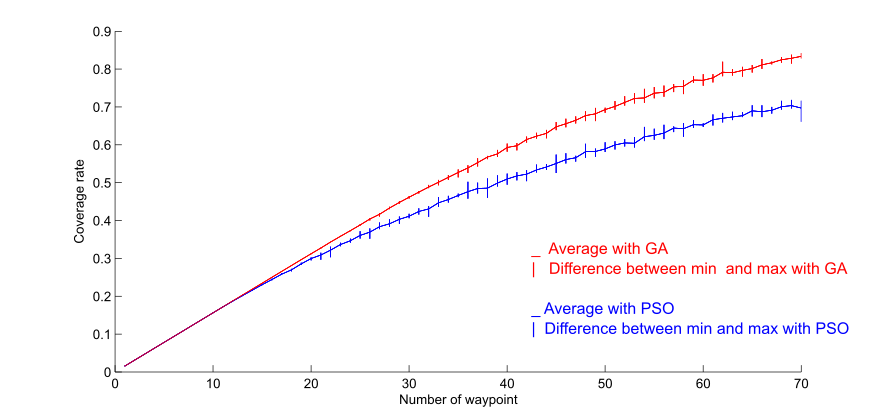
\includegraphics[width=\linewidth]{img/fig8.png}
  \caption{ Comparison of eight solutions given by the GA, with eight solutions given by PSO algorithms with a fixed altitude ($z$ equal to 1) in the big room 240x160. The ground truth for this room equals to 64.}\label{fig:bigRz1}
   \endminipage\hfill
\end{figure}
%
%
\begin{figure}[!]
\minipage{0.99\textwidth}
  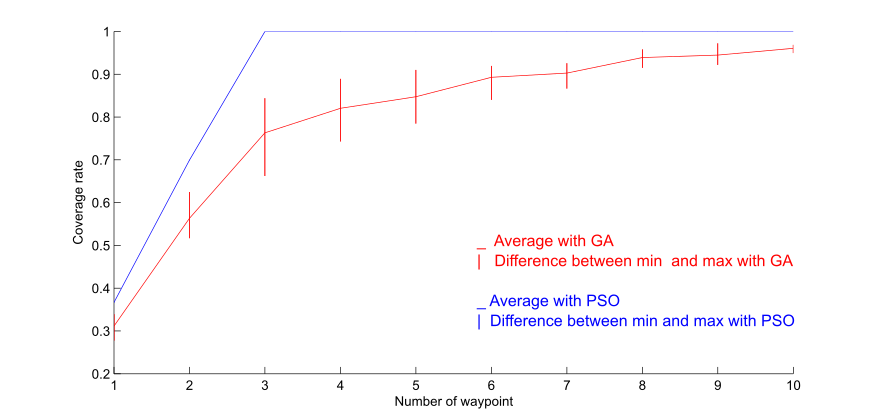
\includegraphics[width=\linewidth]{img/fig9.png}
  \caption{Comparison of eight solutions given by the GA, with eight solutions given by PSO algorithms with a Z between [1/2; 2] in the room with L shape 120x80 and ground truth equal to 15.}\label{fig:RLz2}
   \endminipage\hfill
\end{figure}
After performing the several experiments (see Table \ref{table:table1}), it appears that the GA and PSO algorithms are close in performance in numerous case. Among several experiment of the DoE some particularity appear despite the globally close result of GA and PSO. Also as expected the RS is always the worst solution.
 In the following subsection  just few experiment are taken to illustrate some interesting phenomena specific to the GA and PSO for our problems.

In the case where the search space is large and numerous dimension have to be optimized the GA appear globally more efficient as in Figure \ref{fig:bigRz1}. In contrary in this case (big room with z=1) the PSO give a very bad answer close then simple RS.
%What is appearing in some case as in Figure \ref{fig:bigRz1} is the  GA is much more efficient where the search space is large (big room and big number of cameras),  as the example in Figure \ref{fig:bigRz1}. 
 Instead, PSO is more effective for optimizing small areas as in Figure \ref{fig:RLz2}. In the small room in L shape with a $z$ between 1/2 and 2, the PSO reach quickly (quicker then the 10 000 calls) to the optimal solution. Where here the optimal solution is known and equal to GT. In the same case the GA propose an optimized solution (compared then the RS) but far from the PSO.
 
 This efficiency can be explained by the small variation of the solution introduced by the PSO. However, this small variation is not enough to find an optimized solution in a big search space that occurs when many cameras are required or when the local minimum is deeper. The PSO appear really efficient in a relatively small search space where the number of dimension to optimize is not to high.
 On the other hand the variety  introduced by the GA allows the escape from local minima. This variety is helpfully  in the big search space in order to explore quickly a wide part of it. The variety introduced by the GA became an handicap for a more fine optimization. That explain the bad result obtained during the experiment is a small room. Variety of the GA negatively affect the accuracy of the solution and may require a further optimization step to refine. 
 
%-------- ajouté un exemple entre 2 forme differente qui on un resulta proche 
------------ file Grafig roomShape.txt-----\\
The DoE have been design with different shape in order to see the impact of it on the algorithms. What is appearing during the experiment is the low impact of the shape on the result of the algorithms. The experiment made in the small room (120X80) and the small room in L shape with a z between [1/2; 2](see Figure !!! and Figure !!!). The graphics (see Figure !!! and Figure !!!)  present a similar result, proof of the small impact of the shape on the algorithms.
 This small impact can be explained by the use of meta-heuristic (as PSO and GA) and not by the use of an heuristic  much more dependent of the shape (and the constraint). 
 
Thanks to that we know the two algorithms can be used for a more complex shape as that will be presented in the following experiment.

 





% Following the comparison of the 2 algorithms, the GA seems more suited for finding UAV waypoints especially if it navigates in a large room or  outdoor scenes.
%Furthermore, our comparative study demonstrates that the GA is less dependent on the shape of the area to cover. \\
%------------------
%According to the previous results, the genetic algorithm will be used during future work with no restriction at the convergence point to optimize the positioning of the waypoints in the bigger areas seen in Section  \ref{coverageOutDoor} such as in Figure \ref{subfig:satimg+mask}.\\
%---------------

%fill with the jirs 
%	\subsection{DoF Design of Experiment}
%	\subsection{Result}
%	\subsection{Explication}

\section{Hybrid GA PSO}
% ref: 76* 77* 
 

% l'hybridration peut permetre de tiré avantage des 2 algo
% \begin{itemize}
%  \item interer de l'hybridation (avantage du PSO sur l'optimisation locale et du GA) 
% \item les forme d'ibridation possible 
% \item la plus aproprier dans notre cas et pourquoi 
% \item les experience ( the experimentation  was done in the Big room in L shape as the \ref{fig:Rooms_shapes}.e)
% \item les resultats
% \end{itemize}
Thanks to the experiment done and presented in the previous section (see \ref{sec:GAvsPSO}) the GA and PSO are two algorithms efficient and complementary to solve the problem of camera positioning in the complex and potentially vast area.
  To summarize the previous comparison, it is  difficult to rank the two algorithms in all the environments. GA and PSO have both advantages depending on the area and the number of cameras. GA is better in the big search space and several dimension to optimize when PSO is efficient to refined  faster the solution.
 The hybridization can be the solution to optimize the camera positions in all the condition. The aims of the hybridization is to exploit the better of both algorithms, trying to further refine the solution 77*\cite{c13}.

  
\subsubsection{The different hybridization}

In Premalatha al et 76*  propose tree different solution to hybrid the GA and PSO: 
\begin{itemize}
\item  GA and the PSO are used in parallel. The best solution between both algorithms is used into the other algorithm. 
For example: If the best solution at the end of the first generation is from PSO, this solution is used as a new individual for the crossover on the GA. Or if the best solution is from the GA, this good individual is used in PSO as best particle for the next draw. This operation continue until the convergence of both algorithm.   
%(LA MEILLEURE SOLUTION DES DEUX EST INJECTEE DANS L'AUTRE : CA VEUT DIRE QUOI ? ET TEL QUE DECRIT, CE N'EST PAS DU PARALLELE ! MIEUX EXPLIQUER)
 
\item The GA is used to introduce variety on the PSO, when the PSO is stagnating. The stagnated state are reach when no solution upgrades after a predefined number of iteration. In this case the GA introduces variety by proposing an other solution to PSO. This hybridization have to be manage carefully due to this high risk of non convergence. 

\item The GA is used until the convergence point. When the GA converge to a solution, the PSO is used to refine  with one more optimization. This solution is costly in time due to this double optimization and this double convergence. Finally this hybridization uses the GA optimization as an initialization for the PSO.\\
\end{itemize}

The last hybridization using GA as initialization for PSO is probably one of the most suitable for the problems of camera positioning in a large area. 
Based on the previous experiment the  GA operated efficiently  and required to develop a  %good and need to have help for refined 
solution.  %(PHRASE A REVOIR). 
In this case the GA can be a very good initial guess for the PSO. \\


%the GA and PSO in the precedent subsection. That mean GA and PSO are configure for have the best result depending to the condition and cost function is use a same number of time by the 3 different  algorithms. The hybridation is compare with the  GA and PSO  in fig ??


\subsubsection{Experimentation}
To compare the efficiency of the hybridization GAPSO to the GA, one experimentation is proposed.
The experimentation followed the rule fixed during the comparison as in Table \ref{table:table1}. %\\
It appears the big room in L shape as the Figure \ref{fig:Rooms_shapes}.e is the most suitable to test the hybridization. % (POURQUOI ???).
The L shape room proposes a big search space which can requires a big amount of cameras to cover it. This configuration is the most likely to be improved on different situation, also closer to a realistic configuration.\\
The proposed experiment use the GA for 100 generations and the GA solution as a initialization for the PSO. Also the PSO is lock at 100 iterations. %(C'EST L'EXPERIMENTATION QUI PROPOSE ?). \\%Finally the GAPSO are used for an amount around 20000 call of the cost function or the GA use onnly 10000call but the result of GA wiht 20 000 call are similaire then the 10000 (show fig). like that the encreasing is due to the hibridization and not to the morte time computation allowed. 
 \subsubsection{Result}
  
%\begin{figure}[t]
%\minipage{0.95\textwidth}
%  \includegraphics[width=\linewidth]{HibridLroomGAPSO2.png}
%  \caption{GA vs GAPSO.
%}\label{fig:GAPSO}
%  \endminipage\hfill
%\end{figure}
\begin{figure}[t]
\minipage{0.85\textwidth}
  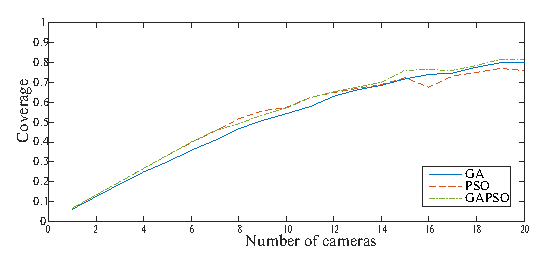
\includegraphics[width=\linewidth]{img/GAPSO_GA_PSO3.eps}
  \caption{comparison between GA PSO and the hybridization of GAPSO.
}\label{fig:GAPSO}
  \endminipage\hfill
\end{figure}
	It appears in the Figure \ref{fig:GAPSO} the hybridization of GAPSO increases slightly the percentage of coverage%(around 0.0002 and 0.107 point of percentage)
. This refinement is due to the PSO ability to optimize the local solution. As we saw previously the GA is efficient in the big search space and with a big amount of dimension to optimize, but the solution gives the GA need some local adjustment to be better. The GA has few limitation to go deeper in the optimization process but this weakness is partially corrected by the hybridization. The principal advantage hybridization is the ability to keep the benefit of both algorithms. The Figure \ref{fig:GAPSO} show that the GAPSO proposes most of the time the best solution or equal to the best solution by combining the advantage of both algorithms. 
	\subsection{memetic ???}
		\subsubsection{DoF}
		\subsubsection{Result}
		\subsubsection{Conclusion}
		
\section{Experiment}
	\subsection{No obstacle }
	\subsection{Rectangle obstacle}
	\subsubsection{With mask}
	\subsection{For big area}
		\subsubsection{map 1}
		\subsubsection{map2 torcy}
		\subsubsection{map3 calvisson}
		


%%%%%%%%%%%%%%%%%%%%%%%%%%%%%%%%%%%%%%%%%%%%%%%%%%%%

 



\chapter{Cover path planning project } 


\minitoc


\section{Splitting the problem }
	Splitting the problem 
			\subsection{Positioning of the waypoint }
			\subsection{Number of waypoint }
			\subsection{Sorted waypoint}
				\subsubsection{Graph theory multi objective  }
				\subsubsection{TSP solution }
				\subsubsection{GA}
			\subsection{Experiment }
		
\section{Use GA with non splitting in sub problem }
		\subsection{Explosion  de la complexité }
		\subsection{Result }
Use GA with non splitting in sub problem
			Explosion  de la complexité 
			Result 

%%%%%%%%%%%%%%%%%%%%%%%%%%%%%%%%%%%%%%%%%%%%%%%%%%%%




% Automatic Lettrine and Minitoc at the begining of the chapter.
%
% The following macros are formatting the text at the begining of a chapter according to the
% standard format.
%
% \chapterintro               See \chapterintrotosection.
%
% \chapterintro*              Similar to \chapterintro, except that the minitoc will be ignored.
%
% \chapterintrotosection      transform to lettrine the first letter that is following this macro
%                             until the next following \section macro.
%                             YOU MUST type the \section macro
%                             in the same file as the \chapterintrotosection macro.
%                             AND
%                             put a minitoc (if the minitoc package is included) just before
%                             the next following \section macro.
%
% \chapterintrotoinput        transform to lettrine the first letter that is following this macro
%                             until the next following \input macro.
%                             YOU MUST type the \input macro
%                             in the same file as the \chapterintrotoinput macro.
%                             AND
%                             put a minitoc (if the minitoc package is included) just before
%                             the next following \input macro.
%
% \chapterintrotoinclude      transform to lettrine the first letter that is following this macro
%                             until the next following \include macro.
%                             YOU MUST type the \include macro
%                             in the same file as the \chapterintrotoinclude macro.
%                             AND
%                             put a minitoc (if the minitoc package is included) just before
%                             the next following \include macro.

%\chapterintro*
%\chapterintro
%\chapterintrotosection
%\chapterintrotoinput
%\chapterintrotoinclude


\section{Proposer une définition}

La définition~\ref{def:unethese} illustre la proposition d'une définition.

\begin{definition}[Une thèse] \label{def:unethese}
Ouvrage présenté devant un jury universitaire pour l'obtention d'un doctorat.
\end{definition}


\section{Inclure un tableau}

Le référencement de la table peut être réalisé à l'aide des macros:
\begin{verbatim}
\tabref{labelid}
\tabpageref{labelid}
\end{verbatim}

\subsection{Exemple 2}

La table \tabref{exampletable2} est un exemple de table avec 5 colonnes, et dans laquelle le titre de la table a été également ajouté en sommet.
\begin{mtable}[ht]{.9\linewidth}{5}{|l|X|l|X|X|}{Titre de la table}{exampletable2}
	\captionastitle % Affiche le titre de la figure en sommet de table
	\tabularheader{Col1}{Col2}{Col3}{Col4}{Col5}
	a & b & c & d & x \\
	\hline
	e & f & g & h & z \\
\end{mtable}



Vous pouvez placer un texte \textup{en exposant}. Vous pouvez placer un texte \textdown{en indice}.

Vous pouvez mettre en avant \emph{un texte}, ou le mettre \Emph{encore plus en avant}.

Vous pouvez formatter les noms de personnes de manière uniforme, comme par exemple \makename{Stéphane}{Galland} 




 
%% Citation from the general bibliography
%\cite{key}
 
%% Citation from the PERSO bibliography
%\citePERSO{key}
 


\section{Détails de la contribution}

\section{Conclusion}
 
\section{Bilan}

\section{Perpectives}
 
%%--------------------
%% Start the end of the thesis
\backmatter
 
%%--------------------
%% Bibliography
 
%% PERSONAL BIBLIOGRAPHY (use 'multibib')
 
%% Change the style of the PERSONAL bibliography
%\bibliographystylePERSO{phdthesisapa}
 
%% Add the chapter with the PERSONAL bibliogaphy.
%% The name of the BibTeX file may be the same as
%% the one for the general bibliography.
%\bibliographyPERSO{biblio.bib}
 
%% Below, include a chapter for the GENERAL bibliography.
%% It is assumed that the standard BibTeX tool/approach
%% is used.
 
%% GENERAL BIBLIOGRAPHY
 
%% To cite one of your PERSONAL papers with the style
%% of the PERSONAL bibliography: \cite{key}
 
%% To force to show one of your PERSONAL papers into
%% the PERSONAL bibliography, even if not cited in the
%% text: \nocite{key}
 
%% The following line set the style of
%% the GENERAL bibliogaphy.
%% The "phdthesisapa" is a "apalike" style with the following
%% differences:
%% a) The titles are output with the color of the institution.
%% b) The name of the PhD thesis' author is underlined.
%\bibliographystyle{phdthesisapa} %!!!!!!%
%% The following line may be used in place of the previous
%% line if you prefer "numeric" citations.
%\bibliographystyle{phdthesisnum}

%% Link the GENERAL bibliogaphy to a BibTeX file.

\bibliography{content/biblio/refManuel1}
%\bibliographystyle{phdthesisapaunsort}
\bibliographystyle{unsrt}
%\bibliographystyle{phdthesisapa}


%%--------------------
%% List of figures and tables
 
%% Include a chapter with a list of all the figures.
%% In French typograhic standard, this list must be at
%% the end of the document.
\listoffigures
 
%% Include a chapter with a list of all the tables.
%% In French typograhic standard, this list must be at
%% the end of the document.
\listoftables
 
%%--------------------
%% Include a list of definitions
\listofdefinitions

%%--------------------
%% Appendixes
\appendix
\part{Annexes}
 
%\include{content/Glosaire/glossaire}
\chapter{Premier chapitre des annexes}

Computation to compute the $\eta, \upsilon$. Where $\eta, \upsilon$ are the horizontal and vertical camera field of view.
	\begin{equation} \label{eq:etaUpsilon}
 	 \begin{split}
		\eta = 2\times \tan^{-1} (\frac{Sw}{(2\times f)}  ) 
 	   \\
		\upsilon = (\frac{Sw}{Sh} )\times \eta
 	 \end{split}
	\end{equation}
	The Equation \ref{eq:etaUpsilon} is to complete the Figure \ref{fig:cam_proj}.
 
\end{document}
